%% Lehmer's totient problem and the companion equation phi(n) | n+1
\documentclass[11pt,reqno]{amsart}

\usepackage[T1]{fontenc}
\usepackage{lmodern}
\usepackage{amsmath,amssymb,amsthm,mathtools}
\usepackage[kerning=true]{microtype}
\usepackage{enumitem}
\usepackage[margin=1.12in]{geometry}
\usepackage{booktabs,array}
\usepackage{graphicx}
\usepackage{xcolor}
\usepackage[colorlinks=true,linkcolor=blue!55!black,citecolor=blue!55!black,urlcolor=blue!55!black]{hyperref}

\numberwithin{equation}{section}

\theoremstyle{plain}
\newtheorem{theorem}{Theorem}[section]
\newtheorem{lemma}[theorem]{Lemma}
\newtheorem{proposition}[theorem]{Proposition}
\newtheorem{corollary}[theorem]{Corollary}
\theoremstyle{remark}
\newtheorem{remark}[theorem]{Remark}

%% Zenodo DOI of the code archive (release v2.3.0).
\newcommand{\zenododoi}{10.5281/zenodo.23072268}

\title[Lehmer's totient problem]
{Lehmer's totient problem with fewer than sixteen prime factors}

\author[P. Mandal]{Priyabrata Mandal\textsuperscript{*}}
\address{Department of Mathematics, Bioinformatics and Computer
  Applications, Maulana Azad National Institute of Technology Bhopal,
  Bhopal 462003, India}
\email{priyabrata@manit.ac.in}
\urladdr{\textnormal{ORCID
  \href{https://orcid.org/0000-0001-6472-6239}{0000-0001-6472-6239}}}

\author[D. Bhattacharjee]{Deep Bhattacharjee}
\address{Formerly, Electro-Gravitational Space Propulsion Laboratory (EGSPL),
  Bhubaneswar, Odisha 751030, India}
\email{d.bhattacharjee@erl-forschung.de}
\email{itsdeep@live.com}
\urladdr{\textnormal{ORCID
  \href{https://orcid.org/0000-0003-0466-750X}{0000-0003-0466-750X}}}

\author[U. Bhattacharya]{Ushashi Bhattacharya}
\address{Formerly, National Taiwan University, Taipei 106319, Taiwan}
\email{rai.bhattacharya.in@gmail.com}
\urladdr{\textnormal{ORCID
  \href{https://orcid.org/0009-0002-2254-3914}{0009-0002-2254-3914}}}

\thanks{\textsuperscript{*}\,Corresponding author: Priyabrata Mandal.}

\subjclass[2020]{Primary 11A25; Secondary 11Y70, 11A51}
\keywords{Euler's totient function, Lehmer's totient problem,
Fermat primes, exhaustive search, formal verification}
\date{}

\begin{document}

\begin{abstract}
We prove that a composite number whose totient divides one less than
the number has at least sixteen distinct prime factors. For the
companion problem, in which the totient divides one more than the
number, we find every solution with at most eight prime factors and
show that a solution prime to three has at least sixteen. Except for
two, the known solutions of the companion problem are exactly the
numbers obtained from one by adjoining one or two primes at a time.
\end{abstract}

\maketitle

%%==================================================================
\section{Introduction}\label{sec:intro}
%%==================================================================

\subsection{Two questions of Lehmer}
Every prime $p$ satisfies $\varphi(p)=p-1$, and so $\varphi(p)$ divides
$p-1$. In 1932 Lehmer \cite{Leh32} asked whether any composite number
$n$ has the same property,
\begin{equation}\label{eq:first}
  \varphi(n)\mid n-1 .
\end{equation}
Nobody has found one, and nobody has shown that none exists. Lehmer
proved that a composite solution of \eqref{eq:first} must be odd,
squarefree and divisible by at least seven distinct primes. The
question is Problem~B37 in Guy's collection \cite{Guy04}. Lehmer's
paper also lists solutions of the companion equation\footnote{The
comments to sequence A050474 of the OEIS \cite{OEIS} record this, and
a misprint in Lehmer's summary where $3\cdot5\cdot353\cdot929$ stands
for $83623935=3\cdot5\cdot17\cdot353\cdot929$.}
\begin{equation}\label{eq:second}
  \varphi(n)\mid n+1 .
\end{equation}
The two equations look alike and behave differently.
Equation~\eqref{eq:first} has no known composite solution. Equation
\eqref{eq:second} has the solutions
\begin{equation}\label{eq:known}
  1,\ 2,\ 3,\ 15,\ 255,\ 65535,\ 83623935,\ 4294967295,\
  6992962672132095,
\end{equation}
and no others are known. Apart from $1$, $2$ and $3$, each of them
satisfies $n+1=2\varphi(n)$. Four of them are products of consecutive
Fermat primes\footnote{The Fermat numbers $F_i=2^{2^i}+1$ are prime
for $0\le i\le4$, and $F_0F_1\cdots F_{r-1}=2^{2^r}-1$. For $r\le5$
the number $n=2^{2^r}-1$ is therefore a product of primes $F_i$, and
$\varphi(n)=2^{1+2+\dots+2^{r-1}}=2^{2^r-1}=(n+1)/2$. The chain breaks
at $r=6$ because $F_5=641\cdot6700417$, as Euler found.}, namely $15=3\cdot5$,
$255=3\cdot5\cdot17$, $65535=3\cdot5\cdot17\cdot257$ and
$4294967295=3\cdot5\cdot17\cdot257\cdot65537$. The other two are
$83623935=3\cdot5\cdot17\cdot353\cdot929$ and
$6992962672132095=83623935\cdot83623937$. These numbers form sequence
A203966 of the OEIS \cite{OEIS}.

Much of the literature on \eqref{eq:first} concerns the number
$\omega(n)$ of distinct prime factors of a composite solution.
Pomerance \cite{Pom77} proved that a composite solution with $k$ prime
factors satisfies $n<k^{2^k}$, so that for each $k$ the question is a
finite one. Cohen and Hagis \cite{CH80} settled all $k\le13$ and
obtained $\omega(n)\ge14$. When $3\mid n$ much more is true: Hagis
\cite{Hag88} proved $\omega(n)\ge298848$, and Burcsi, Czirbusz and
Farkas \cite{BCF11} raised this to $\omega(n)\ge40000000$. In the same
paper they report that a computation of Renze \cite{Ren04}, made
available as a Mathematica notebook, gives $\omega(n)\ge15$ in general,
and Pinch \cite{Pin06} outlined a proof of the same bound in a poster
presented at ANTS~VII. Neither account has been refereed. Since $p-1\mid n-1$ for every prime
$p$ dividing a solution, a composite solution of \eqref{eq:first}
would be a Carmichael number;\footnote{By Korselt's criterion a
composite $n$ satisfies $a^{n-1}\equiv1\pmod n$ for every $a$ prime to
$n$ exactly when $n$ is squarefree and $p-1\mid n-1$ for every prime
$p\mid n$. A solution of \eqref{eq:first} is squarefree by
Lemma~\ref{lem:basic}, and $p-1\mid\varphi(n)\mid n-1$.} Banks, Nevans and Pomerance \cite{BNP09}
discuss this and the connection with Giuga's conjecture.

For \eqref{eq:second} the literature is thinner. The comments to
sequences A050474 and A203966 of the OEIS \cite{OEIS} report that the
M.Sc.\ thesis of Wong \cite{Won97} shows that a further solution of
$n+1=2\varphi(n)$ would need at least eight prime factors, that there
are no further solutions of $n+1=2\varphi(n)$ below $10^{31}$ and none
of \eqref{eq:second} below $1.6\cdot10^{30}$ (Alekseyev), and that
$(n+1)/\varphi(n)=3$ would force at least $33$ prime factors. None of
this has appeared in a refereed paper, and we know of no refereed bound
on $\omega(n)$ for \eqref{eq:second}.

\subsection{Results}
We write $\omega(n)$ for the number of distinct prime factors of $n$.
Our first theorem goes one prime further than the bound announced by
Renze and by Pinch, and its proof contains a complete proof of that
bound, with every step stated and checked.

\begin{theorem}\label{thm:first}
Every composite $n$ with $\varphi(n)\mid n-1$ has $\omega(n)\ge16$.
\end{theorem}

We know of no earlier claim beyond fifteen prime factors.

The other results concern \eqref{eq:second}.

\begin{theorem}\label{thm:eight}
The solutions of $\varphi(n)\mid n+1$ with $\omega(n)\le8$ are exactly
the nine numbers \eqref{eq:known}.
\end{theorem}

\begin{theorem}\label{thm:coprime}
Every solution of $\varphi(n)\mid n+1$ with $n>3$ and $3\nmid n$ has
$\omega(n)\ge16$.
\end{theorem}

\begin{theorem}\label{thm:quotient}
Let $n>3$ satisfy $\varphi(n)\mid n+1$ with $(n+1)/\varphi(n)\ge3$.
Then $\omega(n)\ge33$, and $\omega(n)\ge1540$ if $3\mid n$.
\end{theorem}

The fifth theorem explains the list \eqref{eq:known}. Say that $n$ is a
\emph{Fermat-type} solution if $n+1=2\varphi(n)$; by convention $n=1$
is one.

\begin{theorem}\label{thm:ext}
Let $n_0$ be a Fermat-type solution.
\begin{enumerate}[label=\textup{(\roman*)}]
\item For a prime $q\nmid n_0$, the number $n_0q$ is a Fermat-type
  solution if and only if $q=n_0+2$.
\item For primes $p<q$ not dividing $n_0$, the number $n_0pq$ is a
  Fermat-type solution if and only if
  \[
    (p-n_0-1)(q-n_0-1)=n_0^2+n_0+1 .
  \]
\item The Fermat-type solutions in \eqref{eq:known}, which are all
  of them except $2$, are exactly the numbers obtained from $1$ by
  repeated use of \textup{(i)} and \textup{(ii)}: every such extension
  of one of them is again in \eqref{eq:known}.
\end{enumerate}
\end{theorem}

Theorem~\ref{thm:eight} contains the bound reported from Wong's
thesis and goes one prime factor further: a solution of
\eqref{eq:second} outside \eqref{eq:known} has at least nine prime
factors, whatever the quotient $(n+1)/\varphi(n)$. Theorem~\ref{thm:quotient}
contains the observation on the quotient $3$ recorded in the OEIS. Part (iii) of
Theorem~\ref{thm:ext} places $83623935$ in the same family as the
products of Fermat primes: it is the two-prime extension of $255$
coming from the factorisation $255^2+255+1=65281=97\cdot673$, just as
$4294967295$ comes from the trivial factorisation $65281=1\cdot65281$
(Figure~\ref{fig:tree}).

\subsection{Scope}
Theorems~\ref{thm:first}--\ref{thm:ext} bound the number of prime
factors of a new solution and describe the known ones; they do not
decide whether \eqref{eq:first} has a composite solution or whether
\eqref{eq:second} has solutions beyond \eqref{eq:known}. Section~\ref{sec:walls}
measures the next cases. For \eqref{eq:first} with sixteen prime
factors the number of two-prime problems of the kind solved here grows
from $3.4\cdot10^7$ to about $9\cdot10^{13}$, and for \eqref{eq:second}
with nine prime factors and $3\mid n$ the Fermat primes alone leave
some $10^{17}$ of them. In both cases the cost comes from a few
prefixes whose product $\prod p/(p-1)$ lies extremely close to $2$. Section~\ref{sec:walls} also shows that the
product equation, the size bounds and the congruence conditions used
by the search are satisfied by tuples of integers that are not all
prime (Proposition~\ref{prop:pseudo}), so a proof for all $k$ has to
use primality in an essential way. These tuples all have two entries
divisible by $3$. Tuples with no entry divisible by $3$ do not occur for
$k\le13$, nor for $k\le15$ when all entries but the last three are
prime (Theorem~\ref{thm:pseudo3}), and no congruence condition other
than that of Lemma~\ref{lem:three} can exclude them
(Proposition~\ref{prop:local}). They do occur, for every $k\ge25$
with the sign $+1$ and every $k\ge26$ with the sign $-1$
(Theorem~\ref{thm:pseudo25}), so for Lehmer's equation, and for the
companion equation with $3\nmid n$, a proof for all $k$ has to use the
primality of entries other than $3$.

\subsection{Method}
The proofs of Theorems~\ref{thm:first}--\ref{thm:coprime} combine an
elementary reduction with an exhaustive search. The reduction
(Section~\ref{sec:elem}) shows that in each case one may assume
$n+\varepsilon=2\varphi(n)$, with $\varepsilon=-1$ for Lehmer's
equation and $\varepsilon=+1$ for the companion, and, except in
Theorem~\ref{thm:eight}, that $3\nmid n$. The search
(Section~\ref{sec:search}) chooses the prime factors in increasing
order, confines each one to an interval determined exactly by the
primes already chosen, and determines the last prime from the others
through a divisibility condition. The search was implemented twice, in
different ways, and the two implementations traverse the same tree
node for node. One of them never factors an integer, and its
correctness does not depend on any primality proof. The bounds are
the same for both signs of $\varepsilon$ apart from terms of size
$1/\varphi(n)$, and for $p_1\ge5$ they produce identical trees for all
$k\le14$, and for $k=15$ the same nodes down to depth $13$
(Figure~\ref{fig:profile}). For fifteen primes the last three
are handled together (Section~\ref{sec:three}): once $p_{13}$ is
fixed, the last two primes correspond to a divisor of an explicit
integer in a known residue class, and such divisors are found by
listing the lattice points of a coset near a hyperbola, with a
certified factorisation only in the few cases where the coset is too
dense. This part was implemented twice, and a third, simpler
treatment (Section~\ref{sec:sum}) uses the fact that the two
complementary divisors lie in the same class; it factors nothing, so
that for $k=15$, as for $k\le14$, the conclusion depends on no
primality proof.

The companion equation with eight prime factors and $3\mid n$ behaves
differently. After the Fermat primes $3,5,17,257,65537$ the product
$\prod p/(p-1)$ falls short of $2$ by only $2^{-31}$, the interval for
the sixth prime has length $2^{33}$, and each of the
$1.3\cdot10^8$ admissible choices of that prime leaves a two-prime
problem whose modulus is far below the cube root of the integer to be
split. We treat these problems by the sum route of
Section~\ref{sec:sum}, combined with trial division for the small
divisors and sieved by congruences that primes satisfy, and we settle
the $1967265$ cases in which this would be slow by factoring the integer
completely, with every prime factor proved prime
(Section~\ref{sec:eight}). Theorem~\ref{thm:quotient} is
elementary, and Theorem~\ref{thm:ext} rests on a short identity
together with the factorisation of eight integers.

Every lemma and proposition of Sections~\ref{sec:elem}--\ref{sec:three},
Theorem~\ref{thm:quotient}, Theorem~\ref{thm:ext},
Lemma~\ref{lem:parity}, Propositions~\ref{prop:pseudo}, \ref{prop:local}
and~\ref{prop:lehmerext} and Theorem~\ref{thm:pseudo25} has been verified in the proof assistant
Lean~4 \cite{Lean4} with its mathematical library Mathlib
\cite{Mathlib} (Section~\ref{sec:lean}), and so has every step of the
eight-prime search of Section~\ref{sec:eight} that is not a
computation: the reduction to $n+1=2\varphi(n)$ with $p_1=3$, the
identities behind its two routes, and the soundness of its sieve. The
finite computations inside these proofs, namely the thresholds $7$,
$32$ and $1540$, the factorisations of Table~\ref{tab:ext} and the
primality of its factors, the tuple of Theorem~\ref{thm:pseudo25} and
the $21$ completions of the eight-prime search, are carried out by the
Lean kernel. The exhaustive searches themselves
are not formalised; for them the evidence is the agreement of
independent programs described in Section~\ref{sec:checks}.

The paper is organised as follows. Section~\ref{sec:elem} proves the
reductions and Theorem~\ref{thm:quotient}. Section~\ref{sec:search}
sets up the search and proves that it is complete, and
Section~\ref{sec:three} describes the treatment of the last three
primes. Section~\ref{sec:first} proves Theorem~\ref{thm:first}, and
Section~\ref{sec:second} proves Theorems~\ref{thm:eight},
\ref{thm:coprime} and \ref{thm:ext}. Section~\ref{sec:checks} describes
the checks applied to the computations and the formal verification,
and Section~\ref{sec:walls} the next cases and the pseudo-solutions.

\subsection*{Notation}
Throughout, $n=p_1p_2\cdots p_k$ with primes $p_1<\dots<p_k$, and
$\varepsilon\in\{-1,+1\}$ selects the equation
$\varphi(n)\mid n+\varepsilon$; we put $M=(n+\varepsilon)/\varphi(n)$.
For $0\le j\le k$ let
\[
  A_j=\prod_{i\le j}p_i,\qquad B_j=\prod_{i\le j}(p_i-1),\qquad
  P_j=\frac{A_j}{B_j}=\prod_{i\le j}\frac{p_i}{p_i-1},
\]
with $A_0=B_0=P_0=1$ and $p_0=1$. We write $m=k-j$ for the number of
primes still to be chosen at depth $j$, and
$r_1<r_2<\cdots$ for the primes from $5$ on.

%%==================================================================
\section{Elementary reductions}\label{sec:elem}
%%==================================================================

\begin{lemma}\label{lem:basic}
Let $n>1$ satisfy $\varphi(n)\mid n+\varepsilon$ and put
$M=(n+\varepsilon)/\varphi(n)$. Suppose $n$ is composite if
$\varepsilon=-1$, and $n>3$ if $\varepsilon=+1$.
\begin{enumerate}[label=\textup{(\roman*)}]
\item $n$ is odd, squarefree and composite, and $M\ge2$.
\item For primes $p,q$ dividing $n$, possibly equal, $p\nmid q-1$ and
  $p\nmid M$.
\item $\displaystyle\prod_{p\mid n}\frac{p}{p-1}
  =M-\frac{\varepsilon}{\varphi(n)}$.
\end{enumerate}
\end{lemma}

\begin{proof}
If $n>2$ is even then $\varphi(n)$ is even and $n+\varepsilon$ is odd.
If $p^2\mid n$ then $p$ divides $\varphi(n)$, hence $n+\varepsilon$,
which is impossible since $p\mid n$. For $\varepsilon=+1$ a prime
solution satisfies $n-1\mid2$, so $n\le3$; thus $n$ is composite in
both cases. For odd squarefree composite $n$ we have
$\varphi(n)<n-1$, so $M\ge2$. If $p,q\mid n$ then
$q-1\mid\varphi(n)\mid n+\varepsilon$ while $p\mid n$, so
$p\nmid q-1$; similarly $p\nmid M\varphi(n)=n+\varepsilon$. Finally
$n/\varphi(n)=(n+\varepsilon)/\varphi(n)-\varepsilon/\varphi(n)$.
\end{proof}

The prime $3$ separates the two equations.

\begin{lemma}\label{lem:three}
In the situation of Lemma~\ref{lem:basic}, suppose $3\mid n$. Then
every other prime factor of $n$ is congruent to $2$ modulo $3$, and
\[
  M\equiv\begin{cases}1\pmod3,&\varepsilon=-1,\\
  2\pmod3,&\varepsilon=+1.\end{cases}
\]
Consequently $M\ge4$ if $\varepsilon=-1$, and $M=2$ or $M\ge5$ if
$\varepsilon=+1$. If $M\ge4$ then $\omega(n)\ge1540$.
\end{lemma}

\begin{proof}
For a prime $p\mid n$ with $p\ne3$, Lemma~\ref{lem:basic}(ii) gives
$3\nmid p-1$, so $p\equiv2$ and $p-1\equiv1\pmod 3$. Hence
$\varphi(n)=2\prod_{p\ne3}(p-1)\equiv2\pmod3$, while
$n+\varepsilon\equiv\varepsilon\pmod 3$. The relation
$n+\varepsilon=M\varphi(n)$ becomes $2M\equiv\varepsilon$, which is
the stated congruence. Suppose $M\ge4$. Then $n/\varphi(n)>4$: for
$\varepsilon=-1$ because $n/\varphi(n)=M+1/\varphi(n)$ by
Lemma~\ref{lem:basic}(iii), and for $\varepsilon=+1$ because then
$M\ge5$ and $n/\varphi(n)=M-1/\varphi(n)\ge5-\tfrac12$. On the other hand, if $q_1<q_2<\cdots$ are the
primes congruent to $2$ modulo $3$ from $5$ on, then
\[
  \frac{n}{\varphi(n)}=\frac32\prod_{p\mid n,\;p\ne3}\frac{p}{p-1}
  \le\frac32\prod_{i=1}^{k-1}\frac{q_i}{q_i-1},
\]
since $p/(p-1)$ decreases in $p$. An exact computation in rational
arithmetic shows that the right-hand side first exceeds $4$ at
$k=1540$.
\end{proof}

For $\varepsilon=-1$ this is a weak form of the bounds of Hagis and of
Burcsi, Czirbusz and Farkas mentioned in the introduction; it is short and suffices here. For $\varepsilon=+1$ it shows why $3$ cannot be
removed in the same way: $M=2$ is compatible with $3\mid n$, and each
Fermat prime $5,17,257,65537$ is congruent to $2$ modulo $3$, as are
$353$ and $929$.

\begin{lemma}\label{lem:Mtwo}
In the situation of Lemma~\ref{lem:basic}, suppose $3\nmid n$ and
$\omega(n)\le32$. Then $M=2$.
\end{lemma}

\begin{proof}
All prime factors are at least $5$. By Lemma~\ref{lem:basic}(iii)
and monotonicity,
\[
  M=\frac{n}{\varphi(n)}+\frac{\varepsilon}{\varphi(n)}
  \le\prod_{i\le k}\frac{r_i}{r_i-1}+\frac{1}{\prod_{i\le k}(r_i-1)} ,
\]
where $k=\omega(n)$, since $n/\varphi(n)=\prod_{p\mid n}p/(p-1)$ and
$\varphi(n)=\prod_{p\mid n}(p-1)$, and the $i$-th smallest prime factor
of $n$ is at least $r_i$. An exact computation shows that the
right-hand side is less than $3$ for every $k\le32$. (For $k=32$ the
product is $2.99315\ldots$ and the second term is below $10^{-53}$; at
$k=33$ the product exceeds $3$.) Since $M$ is an integer and $M\ge2$
by Lemma~\ref{lem:basic}(i), $M=2$.
\end{proof}

\begin{corollary}\label{cor:seven}
Let $n>3$ satisfy $\varphi(n)\mid n+1$ with $\omega(n)\le7$. Then
$n+1=2\varphi(n)$.
\end{corollary}

\begin{proof}
With $k=\omega(n)\ge2$ and $s_1<s_2<\cdots$ the odd primes,
Lemma~\ref{lem:basic}(iii) gives, as in the proof of
Lemma~\ref{lem:Mtwo},
$M\le\prod_{i\le k}s_i/(s_i-1)+1/\prod_{i\le k}(s_i-1)$, and the maximum
of the right-hand side over $2\le k\le7$ is $2.92357\ldots<3$. Hence
$M=2$.
\end{proof}

\begin{proof}[Proof of Theorem~\ref{thm:quotient}]
Let $n>3$ with $\varphi(n)\mid n+1$ and $M\ge3$, and let $k=\omega(n)$.
If $3\mid n$, then $M\ge5$ by Lemma~\ref{lem:three}, and the same lemma
gives $k\ge1540$. If $3\nmid n$, then Lemma~\ref{lem:basic}(iii) and
$\varphi(n)\ge\prod_{i\le k}(r_i-1)$ give
\[
  \prod_{i\le k}\frac{r_i}{r_i-1}\;\ge\;\frac{n}{\varphi(n)}
  \;=\;M-\frac1{\varphi(n)}\;\ge\;3-\frac{1}{\prod_{i\le k}(r_i-1)} .
\]
An exact computation shows that this inequality fails for every
$k\le32$ and first holds at $k=33$.
\end{proof}

The case $M\ge3$ of \eqref{eq:second} is therefore far out of reach of
any search, in the same way as the case $3\mid n$ of \eqref{eq:first}.
What remains are the Fermat-type solutions, $n+1=2\varphi(n)$.

%%==================================================================
\section{A branch-and-bound for \texorpdfstring{$n+\varepsilon=2\varphi(n)$}{n+e=2phi(n)}}\label{sec:search}
%%==================================================================

Fix $k\ge2$, a sign $\varepsilon$, and a squarefree odd
$n=p_1\cdots p_k$ with
\begin{equation}\label{eq:M2}
  n+\varepsilon=2\varphi(n).
\end{equation}
By Lemma~\ref{lem:basic}(iii),
\begin{equation}\label{eq:excess}
  \prod_{i=1}^{k}\frac{p_i}{p_i-1}=2-\frac{\varepsilon}{\varphi(n)} .
\end{equation}
For $\varepsilon=-1$ the product lies just above $2$, and for
$\varepsilon=+1$ just below it. Everything in this section is a
consequence of \eqref{eq:excess}, and the two signs are treated
together.

\begin{proposition}\label{prop:below2}
$P_j<2$ for every $j<k$.
\end{proposition}

\begin{proof}
For $\varepsilon=+1$ this is clear, since $P_j\le P_k=2-1/\varphi(n)$.
For $\varepsilon=-1$, suppose $P_j\ge2$ with $j<k$. Since
$p_{j+1}-1<n-1$ we have $p_{j+1}/(p_{j+1}-1)>1+1/(n-1)$, and the
remaining factors exceed $1$, so
$P_k>2\bigl(1+1/(n-1)\bigr)=2+1/\varphi(n)$ by \eqref{eq:M2},
contradicting \eqref{eq:excess}.
\end{proof}

At depth $j$ put $T=2/P_j$, which exceeds $1$ by the proposition, and
\[
  C_j=2B_j-A_j,\qquad T-1=\frac{C_j}{A_j}.
\]
Thus $C_j$ is a positive integer, and $C_j/A_j$ measures how far the
primes chosen so far fall short of the target $2$.

\begin{proposition}\label{prop:bounds}
Let $0\le j\le k-2$, $m=k-j$, $W=(p_j+1)^m$ and
$x=p_{j+1}/(p_{j+1}-1)$. Then
\begin{equation}\label{eq:bounds}
\begin{aligned}
  &x^m>T \quad\text{and}\quad x<T+\frac{1}{A_jW} &&\text{if }\varepsilon=-1,\\
  &x^m\ge T-\frac{1}{A_jW}\quad\text{and}\quad x<T &&\text{if }\varepsilon=+1 .
\end{aligned}
\end{equation}
In particular $p_{j+1}$ lies in an interval $[L_j,U_j]$ whose
endpoints are determined by $p_1,\dots,p_j$, $k$ and $\varepsilon$.
\end{proposition}

\begin{proof}
Let $\rho=\prod_{i>j}p_i/(p_i-1)$. By \eqref{eq:excess},
\[
  \rho=\frac{2-\varepsilon/\varphi(n)}{P_j}
  =T-\frac{\varepsilon}{P_j\varphi(n)} .
\]
There are $m\ge2$ factors in $\rho$; each exceeds $1$ and none exceeds
$x$, because $p/(p-1)$ decreases in $p$. Hence $x<\rho\le x^m$. The
remaining primes are odd and larger than $p_j$ (larger than $2$ when
$j=0$), so $p_i-1\ge p_j+1$ for $i>j$, and
$\varphi(n)=B_j\prod_{i>j}(p_i-1)\ge B_jW$. Therefore
\[
  0<\frac{1}{P_j\varphi(n)}\le\frac{1}{P_jB_jW}=\frac1{A_jW},
\]
and the four inequalities follow from $x<\rho\le x^m$. Finally, for
$\varepsilon=+1$ the quantity $T-1/(A_jW)$ exceeds $1$, since
$T-1=C_j/A_j\ge1/A_j$.
\end{proof}

The inequalities \eqref{eq:bounds} are tested in integers: for instance
$x^m>T$ reads $p^mA_j>2B_j(p-1)^m$. A floating-point estimate is used
only to find a starting point, which is then corrected by exact
comparisons.

\begin{lemma}[congruence prune]\label{lem:prune}
No prime factor of $n$ divides $p-1$ for another prime factor $p$ of
$n$.
\end{lemma}

This is Lemma~\ref{lem:basic}(ii). A candidate $p$ for $p_{j+1}$ is
discarded if $p\mid p_i-1$ or $p_i\mid p-1$ for some $i\le j$.

The last two primes need not be searched separately.

\begin{proposition}\label{prop:last}
Let $A=A_{k-2}$, $B=B_{k-2}$, $C=2B-A$, $p=p_{k-1}$ and $q=p_k$. Then
\begin{equation}\label{eq:last}
  t:=Cp-2B>0,\qquad t\mid Ap+\varepsilon,\qquad
  q=1+\frac{Ap+\varepsilon}{t},
\end{equation}
and equivalently
\begin{equation}\label{eq:hyperbola}
  (Cp-2B)(Cq-2B)=2AB+\varepsilon C .
\end{equation}
\end{proposition}

\begin{proof}
Equation \eqref{eq:M2} reads $Apq+\varepsilon=2B(p-1)(q-1)$. Collecting
the terms in $q$ gives $q\,(Cp-2B)=2B(p-1)+\varepsilon$. The right-hand
side is positive, so $t>0$, and
$q-1=\bigl(2Bp-2B+\varepsilon-Cp+2B\bigr)/t=(Ap+\varepsilon)/t$.
Multiplying $Cpq-2B(p+q)+2B-\varepsilon=0$ by $C$ and completing the
product gives
$(Cp-2B)(Cq-2B)=4B^2-2BC+\varepsilon C=2AB+\varepsilon C$.
\end{proof}

Once $p_1,\dots,p_{k-2}$ are fixed, the prime $p_{k-1}$ runs over the
interval of Proposition~\ref{prop:bounds} with $m=2$, and for each
candidate $p$ the last prime is determined by \eqref{eq:last}.
Alternatively, by \eqref{eq:hyperbola}, $t$ is a divisor of the integer
\[
  D=2AB+\varepsilon C
\]
lying in a known residue class modulo $C$, so the candidates can be
read off from the divisors of $D$ when $D$ can be factored. The first
route costs time proportional to the length of the interval, the
second the cost of factoring $D$. Figure~\ref{fig:search} summarises
the procedure.

\begin{figure}[t]
\centering
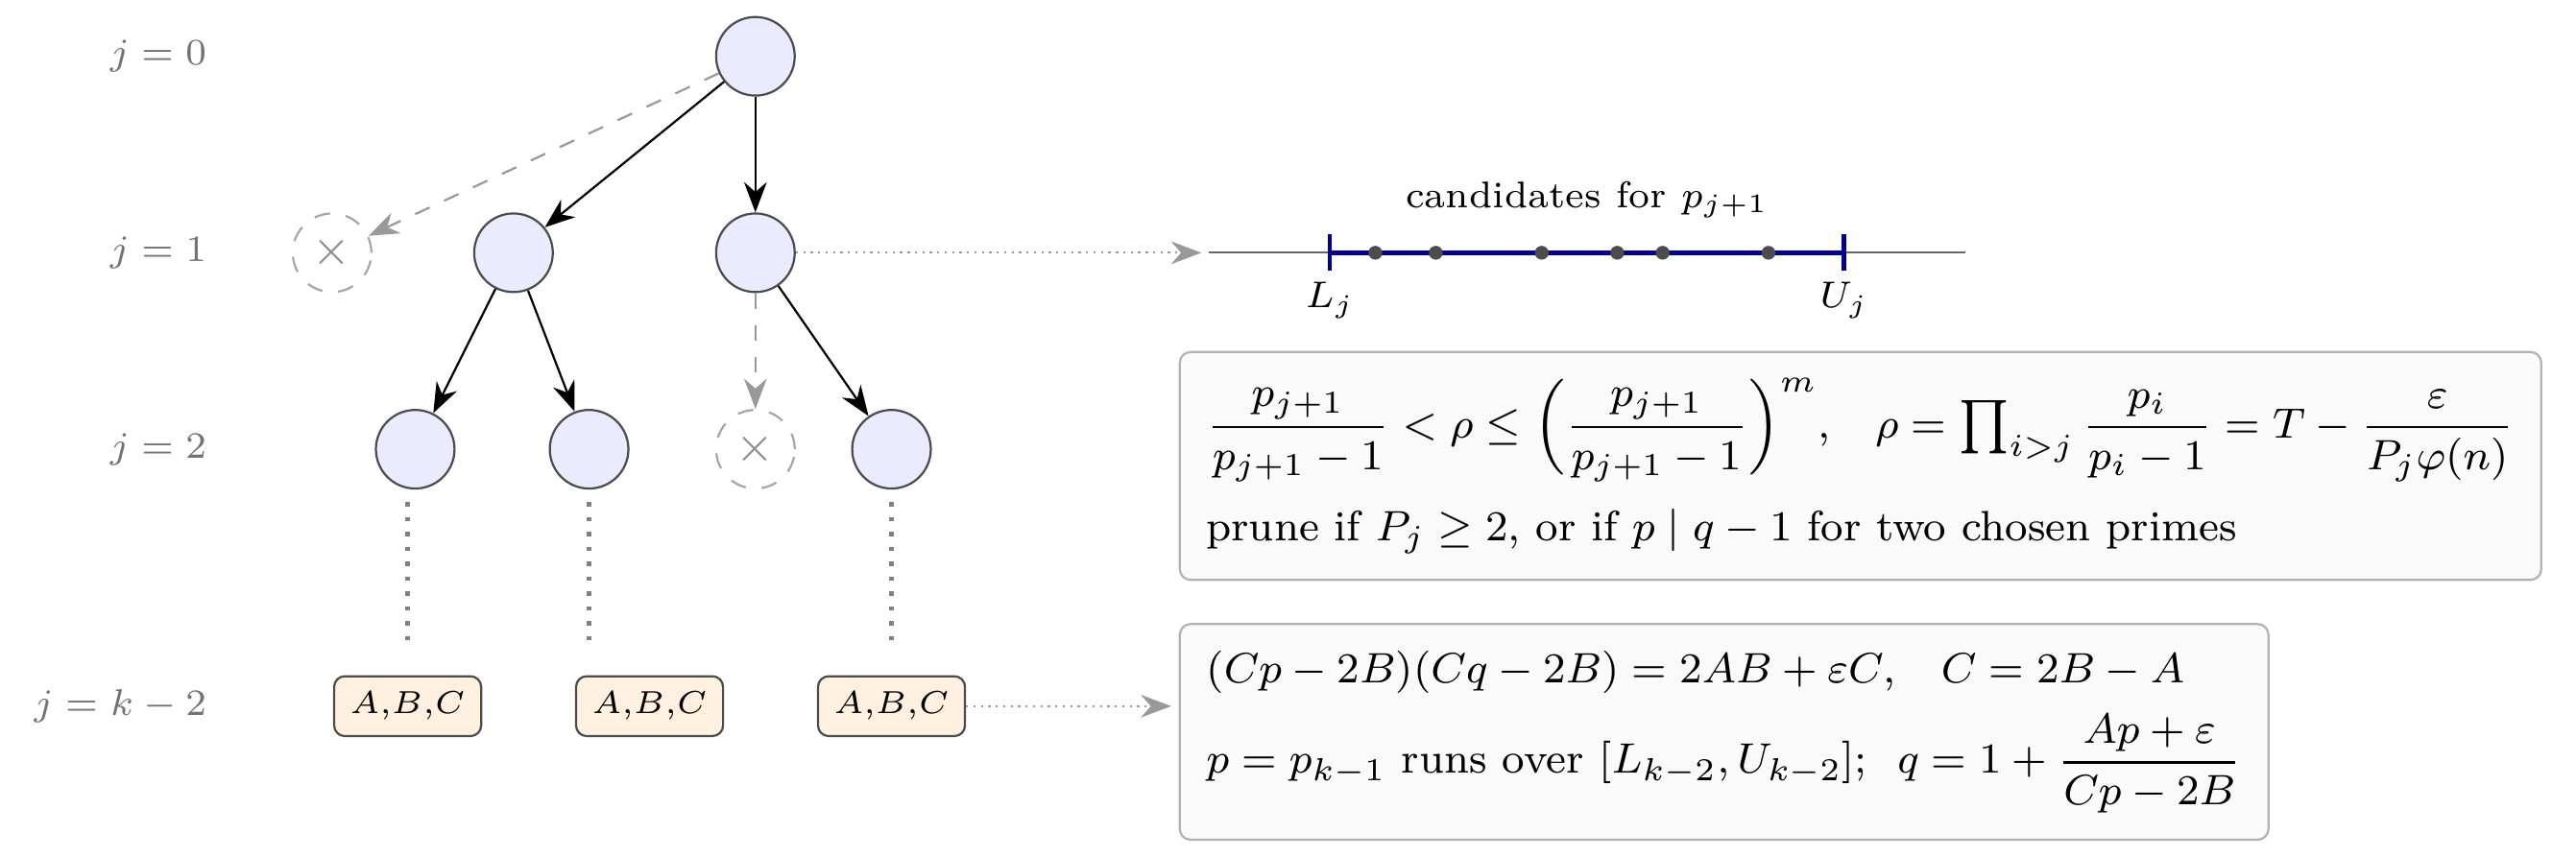
\includegraphics[width=\textwidth]{figures/fig_search.png}
\caption{The search for $n=p_1\cdots p_k$ with $n+\varepsilon=2\varphi(n)$.
A node at depth $j$ is an increasing sequence of primes
$p_1<\dots<p_j$. Its children are the primes in the interval
$[L_j,U_j]$ of Proposition~\ref{prop:bounds} that pass the congruence
prune; dashed branches are cut. At depth $k-2$ the pair
$(p_{k-1},p_k)$ is a lattice point on the hyperbola
\eqref{eq:hyperbola}, found by running $p$ over $[L_{k-2},U_{k-2}]$
or by factoring $2AB+\varepsilon C$.}
\label{fig:search}
\end{figure}

The search is a depth-first traversal of the tree whose nodes at depth
$j\le k-2$ are the increasing sequences $(p_1,\dots,p_j)$ of primes
with $p_1\ge p_{\min}$, where each $p_{i+1}$ lies in the interval
determined by $(p_1,\dots,p_i)$ and passes the congruence prune, and
where $P_i<2$ for all $i\le j$. At depth $k-2$ each candidate
$p_{k-1}$ is tested with \eqref{eq:last}: one checks that $t>0$, that
$t\mid Ap+\varepsilon$, that $q=1+(Ap+\varepsilon)/t$ is a prime larger
than $p$, that $p$ and $q$ pass the congruence prune, and finally that
\eqref{eq:M2} holds exactly.

\begin{theorem}[completeness]\label{thm:complete}
If $n=p_1\cdots p_k$ with primes $p_{\min}\le p_1<\dots<p_k$ satisfies
\eqref{eq:M2}, then the traversal visits $(p_1,\dots,p_{k-2})$,
examines the candidate $p_{k-1}$, and records $n$.
\end{theorem}

\begin{proof}
By induction on $j$ the node $(p_1,\dots,p_j)$ is visited for every
$j\le k-2$: the prime $p_{j+1}$ lies in the interval of
Proposition~\ref{prop:bounds}, it passes the prune by
Lemma~\ref{lem:prune}, and $P_{j+1}<2$ by
Proposition~\ref{prop:below2}. At depth $k-2$ the candidate
$p=p_{k-1}$ satisfies \eqref{eq:last} with $q=p_k$. A primality test
never declares a prime to be composite, so $q$ is accepted, and the
final check of \eqref{eq:M2} succeeds.
\end{proof}

Two points concern rigour. First, all arithmetic is exact:
$A_j$, $B_j$, $C_j$, the interval endpoints and the quantities in
\eqref{eq:last} are integers or ratios of integers compared by cross
multiplication. Second, the probabilistic primality tests used by the
programs\footnote{The programs use the test of the SymPy library
\cite{SymPy}. In the configuration we used, without the optional
gmpy2 package, it is a strong probable-prime test to the thirteen
bases $2,3,\dots,41$ below $\psi_{13}=3317044064679887385961981$,
and a Baillie--PSW test above it. Sorenson and Webster \cite{SW17}
showed that every composite number below $\psi_{13}$ fails the first
test for at least one of these bases, so there it is a proof. The
Baillie--PSW test \cite{BW80,PSW80} combines a strong probable-prime
test to base $2$ with a strong Lucas test; no composite number is
known to pass it. With gmpy2 installed, SymPy applies the
Baillie--PSW test throughout.} can err only by declaring a composite number prime,
never by declaring a prime composite. Such an error could add a node
or accept a composite $q$, but it can never remove an actual solution.
A search that finds nothing is therefore a proof that there is
nothing, and the completeness of the enumeration route depends on no
primality proof. The exact check of \eqref{eq:M2} would not catch such
an error, since it uses $\prod(p_i-1)$ in place of $\varphi(n)$. This
matters only for solutions that are reported, and every solution
reported in this paper, including those of Appendix~\ref{app:known},
has all its prime factors below $10^{14}$, where the tests are
proofs. The divisor route depends on a complete
factorisation of $D$, which is certified whenever $D<\psi_{13}$,
since then every prime factor of $D$ lies below that bound.

%%==================================================================
\section{The last three primes}\label{sec:three}
%%==================================================================

For $k\le14$ the search of Section~\ref{sec:search} is cheap because
the interval for $p_{k-1}$ is never longer than about $5\cdot10^7$. For
$k=15$ this is no longer true. After the prime $p_{13}$ has been chosen
the interval for $p_{14}$ can be longer than $10^{14}$, and there are
tens of millions of choices of $p_{13}$. Neither route of
Section~\ref{sec:search} copes with this: running $p_{14}$ over its
interval is far too slow, and factoring tens of millions of integers of
about fifty digits is a computation of a different order. In this
section we describe two further ways of finding the divisors of
$2AB+\varepsilon C$ that can occur in Proposition~\ref{prop:last}.
Both use the residue class in which these divisors lie: the first
lists lattice points near a hyperbola, and the second scans the
possible values of the sum of two complementary divisors.

\subsection{Reduction to divisors in a residue class}
Fix a node $(p_1,\dots,p_{k-3})$ at depth $k-3$ and a candidate
$s=p_{k-2}$ in its interval that passes the congruence prune. Put
\[
  A'=A_{k-3}\,s,\qquad B'=B_{k-3}\,(s-1),\qquad c=2B'-A',\qquad
  N=2A'B'+\varepsilon c .
\]
If $c\le0$ then $P_{k-2}=A'/B'\ge2$, and by
Proposition~\ref{prop:below2} no solution has $p_1,\dots,p_{k-3},s$ as
its first $k-2$ primes; such $s$ are discarded. So let $c\ge1$. By
Proposition~\ref{prop:last}, applied with $A=A'$ and $B=B'$, the
remaining primes $p<q$ of a solution satisfy
$(cp-2B')(cq-2B')=N$ with both factors positive. Let $r$ be the least
positive residue of $-2B'$ modulo $c$.

By \eqref{eq:excess} the last three primes satisfy
\[
  \frac{s}{s-1}\cdot\frac{p}{p-1}\cdot\frac{q}{q-1}
  =T-\frac{\varepsilon}{P_{k-3}\,\varphi(n)},\qquad T=\frac{2}{P_{k-3}},
\]
so the point $(s,p,q)$ lies next to the surface on which this product
equals $T$. Fixing $s$ cuts the surface in a curve, and the pair
$(p,q)$ lies exactly on the hyperbola $(cp-2B')(cq-2B')=N$ beside that
curve (Figure~\ref{fig:surface}).

\begin{figure}[t]
\centering
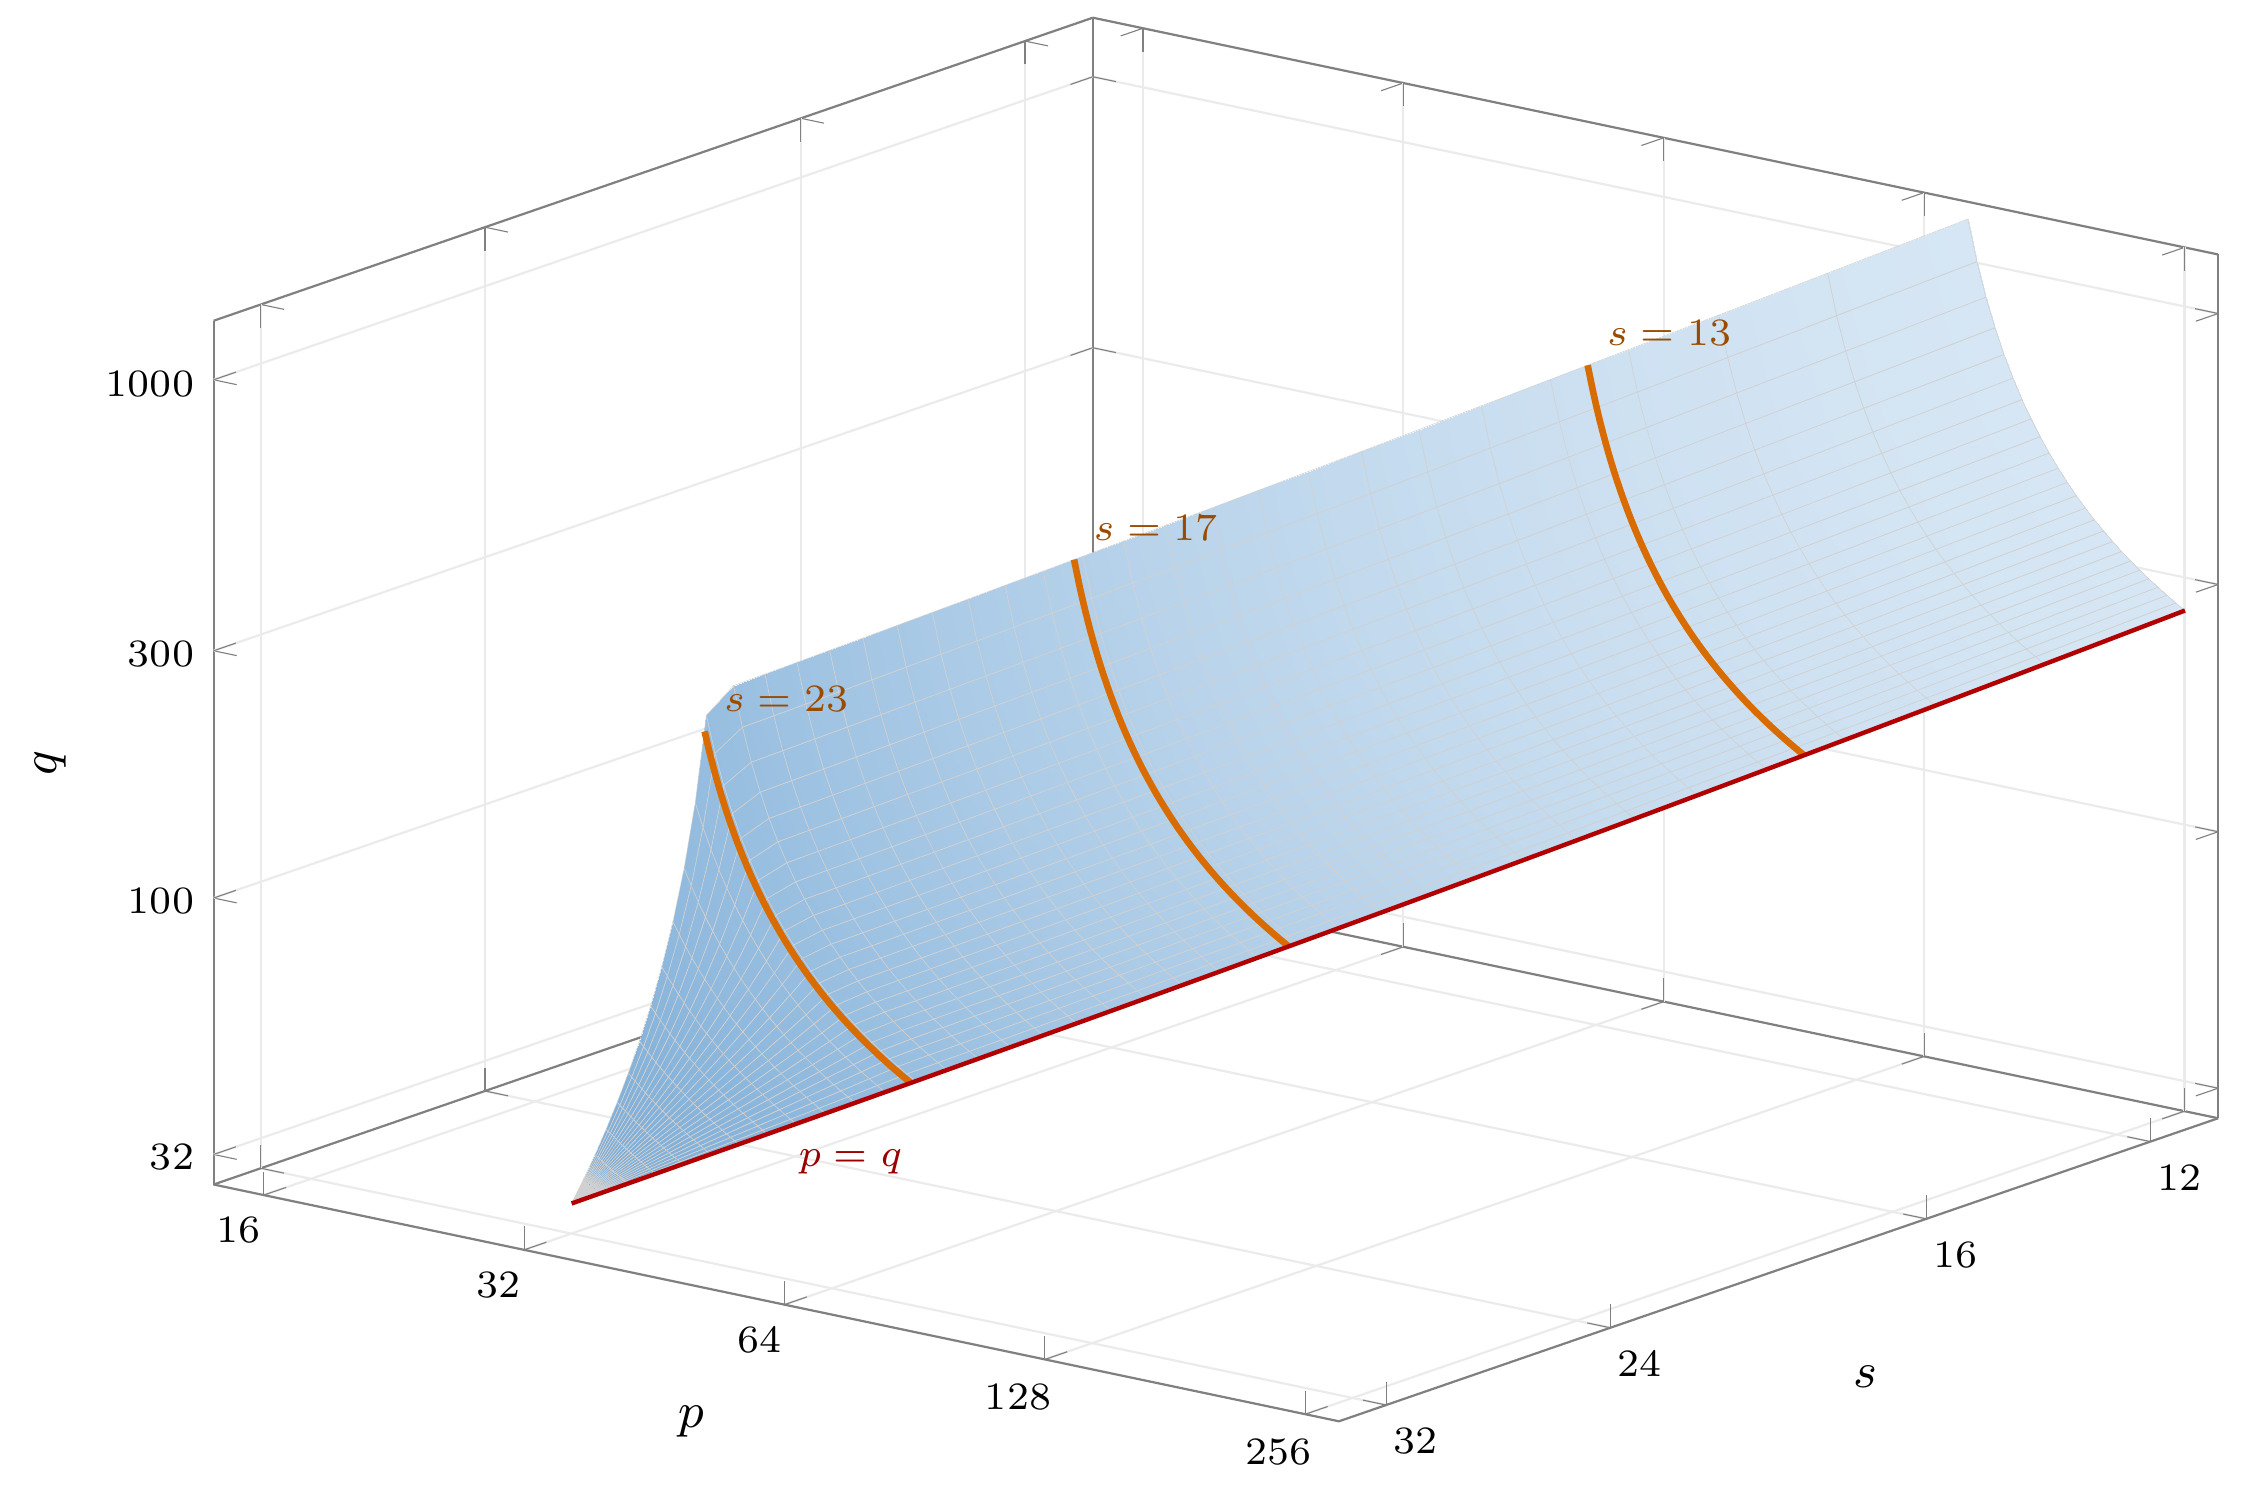
\includegraphics[width=0.86\textwidth]{figures/fig_surface.png}
\caption{The surface $\frac{s}{s-1}\cdot\frac{p}{p-1}\cdot\frac{q}{q-1}=T$
with $s<p<q$, for $T=1.1$ on logarithmic axes. Each slice with fixed
$s$, three of which are marked, falls steeply from large values of $q$
to the edge $p=q$. The slices shrink as $s$ grows, and the surface ends
at the point $s=p=q$ where $(s/(s-1))^3=T$.}
\label{fig:surface}
\end{figure}

\begin{proposition}\label{prop:class}
The integer $t=cp-2B'$ is a divisor of $N$ with
\[
  t\equiv r\pmod c,\qquad 1\le t\le\sqrt N .
\]
Moreover $\gcd(r,c)=1$ and $N\equiv r^2\pmod c$. Conversely, every
divisor $t$ of $N$ with these properties gives integers
$p=(t+2B')/c$ and $q=(N/t+2B')/c$ satisfying
$A'pq+\varepsilon=2B'(p-1)(q-1)$.
\end{proposition}

\begin{proof}
The congruence holds because $t\equiv-2B'\pmod c$, and $t\ge1$ because
both factors are positive, and $t\le\sqrt N$ because $p<q$ makes
$t$ the smaller of the two factors. Since $c=2B'-A'$ we have
$\gcd(2B',c)=\gcd(2B',A')$, which is $1$ because $A'$ is odd and, by
the congruence prune, no prime factor of $A'$ divides $B'$; hence
$\gcd(r,c)=1$. Further $N\equiv2A'B'\equiv(2B')^2\equiv r^2\pmod c$,
using $A'\equiv2B'$. Conversely, let $t$ be such a divisor. Then
$N/t\equiv r^2r^{-1}=r\pmod c$, so both $t$ and $N/t$ are congruent to
$-2B'$ and $p$ and $q$ are integers. Expanding $(cp-2B')(cq-2B')=N$ and
using $4B'^2-2A'B'=2B'c$ gives
$c\bigl(cpq-2B'(p+q)+2B'-\varepsilon\bigr)=0$, which, as $c\ge1$ and
$c=2B'-A'$, is the equation $A'pq+\varepsilon=2B'(p-1)(q-1)$.
\end{proof}

So the two-prime problem at depth $k-2$ becomes the following question:
given $N$, a modulus $c$ and a class $r$ prime to $c$, list the
divisors of $N$ up to $\sqrt N$ that are congruent to $r$ modulo $c$.
Lenstra \cite{Len84} proved that there are at most $11$ such divisors
when $c>N^{1/3}$, and gave a polynomial-time algorithm to find them;
Coppersmith, Howgrave-Graham and Nagaraj \cite{CHN08} extended the
algorithmic side down to $c>N^{1/4+\delta}$. We use a simpler device
which is well suited to our range and whose correctness is elementary,
and in Section~\ref{sec:sum} an even simpler one that exploits the
fact that $t$ and $N/t$ lie in the same class.

\subsection{Lattice points near a hyperbola}
Let $r'$ be the residue of $Nr^{-1}$ modulo $c$, so that $r'=r$ in the
situation of Proposition~\ref{prop:class}, and put
\[
  w=\frac{N-rr'}{c},\qquad \alpha\equiv wr^{-1},\qquad
  \beta\equiv r'r^{-1}\pmod c .
\]
A divisor $t\equiv r$ is written $t=r+cu$ with $u\ge0$, and then
$N/t=r'+cv$ for an integer $v$. Expanding
$(r+cu)(r'+cv)=N$ gives
\begin{equation}\label{eq:uv}
  c\,uv+r'u+rv=w ,
\end{equation}
so the pairs $(u,v)$ are the lattice points on a hyperbola. Reducing
\eqref{eq:uv} modulo $c$ shows that each of them lies in the coset
\begin{equation}\label{eq:coset}
  v\equiv\alpha-\beta u\pmod c .
\end{equation}
The coset has one point in every $c$ consecutive values of $v$ above a
given $u$, so on its own it says little. Its use comes from
combining it with the shape of the hyperbola.

\begin{lemma}\label{lem:box}
Let $0\le u_0\le u_1$ and put
\[
  v^+=\Bigl\lfloor\frac{\lfloor N/(r+cu_0)\rfloor-r'}{c}\Bigr\rfloor,\qquad
  v^-=\Bigl\lceil\frac{\lceil N/(r+cu_1)\rceil-r'}{c}\Bigr\rceil .
\]
If $t=r+cu$ divides $N$ and $u_0\le u\le u_1$, then $N/t=r'+cv$ with
$v^-\le v\le v^+$ and $v$ satisfying \eqref{eq:coset}. Consequently,
with $H=v^+-v^-+1$, the integer $u$ lies in the set
\begin{equation}\label{eq:window}
  \bigl\{\,u\in[u_0,u_1]:\ (\alpha-\beta u-v^-)\bmod c\ <H\,\bigr\},
\end{equation}
and there is no such $t$ at all if $H\le0$.
\end{lemma}

\begin{proof}
Since $t\equiv r\pmod c$ and $\gcd(r,c)=1$, we have
$N/t\equiv Nr^{-1}\equiv r'\pmod c$, so $v=(N/t-r')/c$ is an integer.
The cofactor $N/t$ is an integer between $N/(r+cu_1)$ and
$N/(r+cu_0)$, hence between the ceiling of the first and the floor of
the second, and this gives $v^-\le v\le v^+$; in particular $H\ge1$.
The congruence \eqref{eq:coset} was shown above. Put
$x=(\alpha-\beta u-v^-)\bmod c$, so that $0\le x<c$ and
$v-v^-\equiv x\pmod c$. As $v-v^-\ge0$, it is at least the least
non-negative member $x$ of its class, and so $x\le v-v^-\le H-1$.
\end{proof}

If $H\ge c$ the set \eqref{eq:window} is the whole of $[u_0,u_1]$,
and every $u$ in the box is tested. If $H<c$ it consists of the $u$
for which an arithmetic progression modulo $c$ falls into a window of
length $H$, and its elements can be listed in increasing order without
looking at the others, at a cost of $O(\log c)$ arithmetic operations
each, by the following elementary recursion.

\begin{lemma}\label{lem:firsthit}
Let $0\le a<M$ and $0<L\le R<M$. The least $y\ge0$ with
$L\le ay\bmod M\le R$ is found as follows. If $a=0$ there is no such
$y$. If $a\ge1$ and $a\lceil L/a\rceil\le R$, it is $\lceil L/a\rceil$.
Otherwise it is $\lceil(L+Mz)/a\rceil$, where $z$ is the least integer
$\ge0$ with
\[
  (-R)\bmod a\ \le\ (M\bmod a)\,z\bmod a\ \le\ (-L)\bmod a ,
\]
and if no such $z$ exists there is no $y$. The last problem is of the
same kind, with $(M,a,L,R)$ replaced by
$(a,\,M\bmod a,\,(-R)\bmod a,\,(-L)\bmod a)$.
\end{lemma}

\begin{proof}
If $a=0$ then $ay\bmod M=0<L$ for every $y$. In the second case
$ay\le R<M$ for $y=\lceil L/a\rceil$, so $ay\bmod M=ay\in[L,R]$, while
$0\le ay<L$ for smaller $y\ge0$. Otherwise no multiple of $a$ lies in
$[L,R]$. Since any $a$ consecutive integers contain a multiple of $a$,
this gives $R-L\le a-2$; moreover $a\nmid R$, and no multiple of $a$
lies in $[-R,-L]$, so the residues $(-R)\bmod a,\dots,(-L)\bmod a$ of
$-R,\dots,-L$ increase without wrapping around and
$0<(-R)\bmod a\le(-L)\bmod a<a$. A solution $y$ satisfies $ay=Mz+x$
with $z=\lfloor ay/M\rfloor$ and $x=ay\bmod M\in[L,R]$, and $z\ge1$
because $z=0$ would make $x=ay$ a multiple of $a$ in $[L,R]$.
Conversely, for a given $z\ge0$ a solution with this $z$ exists
exactly when $[L+Mz,R+Mz]$ contains a multiple of $a$; that multiple
is unique, because $R-L<a$, and the solution is
$y=\lceil(L+Mz)/a\rceil$. The
interval contains a multiple of $a$ exactly when $Mz\equiv-x\pmod a$
for some $x\in[L,R]$, that is, when $Mz\bmod a=(M\bmod a)z\bmod a$
lies in the stated range. The intervals $[L+Mz,R+Mz]$ are disjoint
and increase with $z$, since $R-L<M$, so the least $z$ gives the least
$y$.
\end{proof}

The recursion replaces $(M,a)$ by $(a,M\bmod a)$, as in Euclid's
algorithm, so it stops after $O(\log M)$ steps. It is applied with
$M=c$ and $a=-\beta\bmod c$ as follows. Starting from $u=u_0$, let
$b=(\alpha-\beta u-v^-)\bmod c$. If $b<H$, then $u$ is in
\eqref{eq:window}. Otherwise the next element of \eqref{eq:window}, if it
does not exceed $u_1$, is $u+y$, where $y$ is the least integer $\ge0$ with
$c-b\le ay\bmod c\le c-b+H-1$; this window lies inside $[1,c-1]$, so
Lemma~\ref{lem:firsthit} applies. Every $u$ found in this way is
tested by one exact division of $N$ by $r+cu$, and the search resumes
at $u+1$.

\begin{figure}[t]
\centering
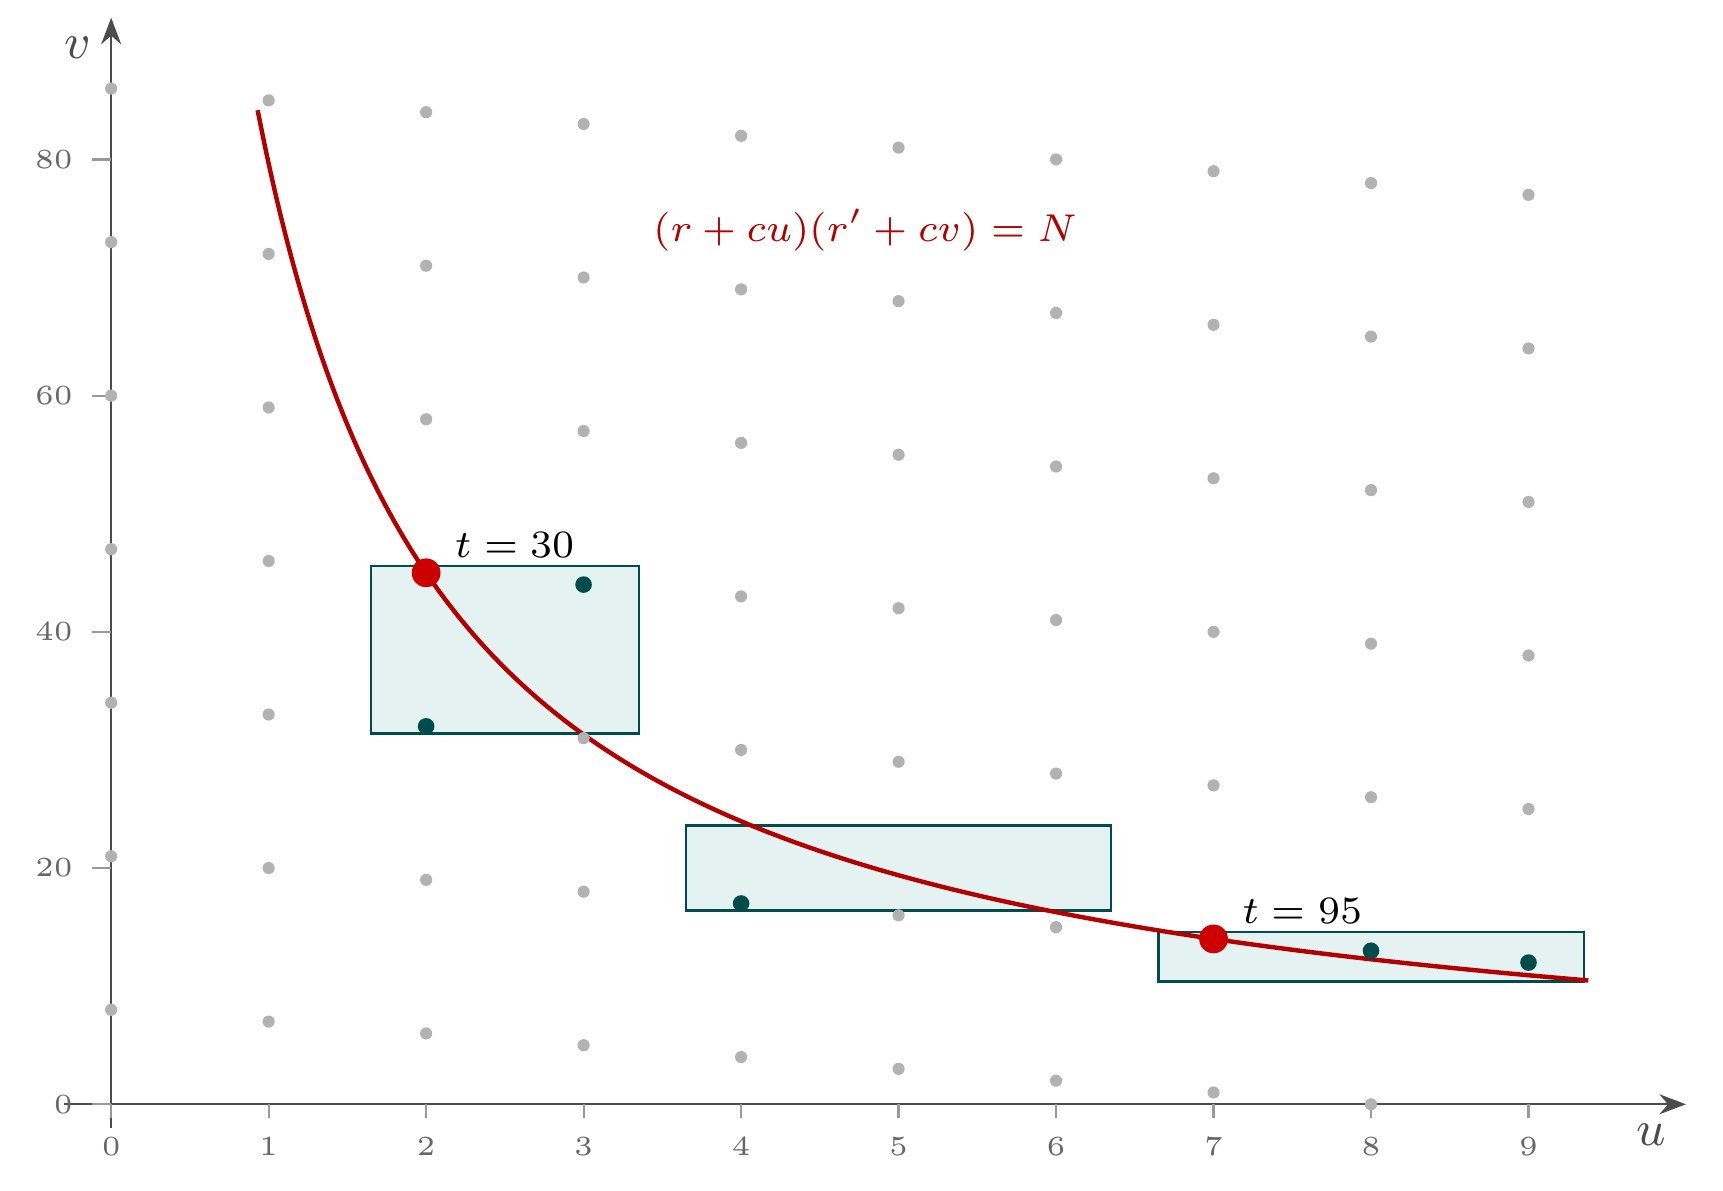
\includegraphics[width=0.69\textwidth]{figures/fig_boxes.png}
\caption{The divisors of $N=17670$ in the class $4$ modulo $13$ up to
$\sqrt N$, found as in Lemma~\ref{lem:box}. The grey points form the
coset \eqref{eq:coset}, here $v\equiv8-u\pmod{13}$; the curve is the
hyperbola \eqref{eq:uv}. The boxes cover the curve for $2\le u\le9$
(the values $u=0,1$ are tested directly), and only the points inside a
box are examined. Two of them lie on the curve and give the divisors
$t=30$ and $t=95$.}
\label{fig:boxes}
\end{figure}

\subsection{Choosing the boxes}
The range $0\le u\le U=\lfloor(\lfloor\sqrt N\rfloor-r)/c\rfloor$ is
cut into consecutive intervals $[u_0,u_1]$, each giving a box
$[u_0,u_1]\times[v^-,v^+]$ in Lemma~\ref{lem:box}
(Figure~\ref{fig:boxes}). Correctness does not depend on how this is
done; the choice only affects the running time. Since
$v\approx K/u$ with $K=N/c^2$, a box with $u_1-u_0=\lambda u_0$ has
area close to $K\lambda^2/(1+\lambda)$, and as the coset has one point
per area $c$ we choose $\lambda$ with $\lambda^2/(1+\lambda)=c^3/N$, so
that each box holds about one point of \eqref{eq:coset}. Two regimes
appear. If $c^3>N$, then $\lambda$ exceeds $1.6$ and grows like
$c^3/N$, so that $O\bigl(\log N/\log(2+c^3/N)\bigr)$ boxes cover the
whole range: this is Lenstra's range, and the work is a handful of
Euclidean recursions. If $c^3<N$,
the boxes shrink to width about $u_0(c^3/N)^{1/2}$, the values of $u$
below $(N/c^3)^{1/2}$ are tested one at a time, and the number of
boxes grows like $(N/c^3)^{1/2}\log N$. When this estimate exceeds a
fixed threshold we factor $N$ completely instead and read off its
divisors in the class.

\begin{theorem}\label{thm:three}
Let $(p_1,\dots,p_{k-3})$ be a node at depth $k-3$ of the search of
Section~\ref{sec:search}. Every $n=p_1\cdots p_k$ with
$n+\varepsilon=2\varphi(n)$ extending this node is found by running
$s=p_{k-2}$ over the admissible primes of its interval and, for each
$s$, listing the divisors of Proposition~\ref{prop:class} by
Lemmas~\ref{lem:box} and~\ref{lem:firsthit} or by a complete
factorisation of $N$.
\end{theorem}

\begin{proof}
The prime $p_{k-2}$ lies in the interval and passes the prune, as in
the proof of Theorem~\ref{thm:complete}. For $s=p_{k-2}$,
Proposition~\ref{prop:class} shows that $t=cp_{k-1}-2B'$ is one of the
divisors listed: Lemma~\ref{lem:box} shows that $u=(t-r)/c$ lies in
the set \eqref{eq:window} of the box that contains it, and
Lemma~\ref{lem:firsthit} lists every element of that set, or, if
$N$ is factored, $t$ is read off from its factorisation. The converse part of
Proposition~\ref{prop:class} then recovers $p_{k-1}$ and $p_k$.
\end{proof}

In practice every divisor that is found yields integers $s<p<q$ with
$A_{k-3}spq+\varepsilon=2B_{k-3}(s-1)(p-1)(q-1)$, and $n$ is a solution
exactly when $p$ and $q$ are prime. As before, the correctness of a
negative answer depends on no primality proof except in the factoring
route, where every prime factor of $N$ is proved prime: below
$\psi_{13}$ by the strong probable-prime test to the first thirteen
prime bases, which is a proof there by the work of Sorenson and
Webster \cite{SW17}, and above it by the primality prover of FLINT
\cite{FLINT}. That prover uses the $n-1$ and $n+1$ methods of
Brillhart, Lehmer and Selfridge \cite{BLS75} when enough of $n-1$ or
$n+1$ can be factored, and otherwise the Jacobi sum test of Adleman,
Pomerance and Rumely \cite{APR83} in the form given by Cohen and
Lenstra \cite{CL84}.

\subsection{A second implementation}
We wrote the method twice. The first implementation follows the
description above: its boxes are intervals in $u$, and the candidates
in a box come from Lemma~\ref{lem:firsthit}. The second takes its
nodes at depth $k-3$ from the rational bounds of the first program of
Section~\ref{sec:checks}, generates the primes $s$ by a different
routine, cuts the hyperbola into boxes along $v$ rather than $u$, and
lists the points of the coset in a box from a basis of the lattice
$\{(u,v):r'u+rv\equiv0\pmod c\}$ that is Lagrange-reduced for the norm
in which the box is a square;\footnote{A basis $e_1,e_2$ of a plane
lattice is Lagrange-reduced for a positive definite quadratic form $Q$
when $Q(e_1)\le Q(e_2)\le Q(e_2\pm e_1)$. For a box with sides $w_u$
and $w_v$ the program takes $Q(u,v)=(w_vu)^2+(w_uv)^2$, writes the
four corners of the box in the coordinates of the reduced basis, and
runs over the integer points of the smallest rectangle that contains
them. Since the box is convex, this rectangle contains the coordinates
of every lattice point in the box whatever the basis; the reduction
only keeps the rectangle small.} a point is accepted when it satisfies
\eqref{eq:uv} exactly. It switches to factoring at a lower threshold,
and it certifies every prime factor with FLINT. The two share no code
beyond the arithmetic libraries.

\subsection{The sum of the two factors}\label{sec:sum}
The classes of Proposition~\ref{prop:class} are special: $t$ and $N/t$
lie in the same class modulo $c$, because $N\equiv r^2$. This allows a
third treatment which uses neither boxes nor factoring. Write $t=r+cu$
and $N/t=r+cv$ with $0\le u\le v$, and put $m=(N-r^2)/c$. Then
\begin{equation}\label{eq:sum}
  c\,uv+r\,(u+v)=m ,
\end{equation}
so the sum $S=u+v$ lies in the single class $S\equiv mr^{-1}\pmod c$,
and $u$ and $v$ are the roots of $X^2-SX+(m-rS)/c$. Conversely, if
$S\equiv mr^{-1}\pmod c$, then $(m-rS)/c$ is an integer, and if
$S^2-4(m-rS)/c=e^2$ with an integer $e\ge0$ of the parity of $S$, then
$u=(S-e)/2$ and $v=(S+e)/2$ are integers satisfying \eqref{eq:sum}, so
that $(r+cu)(r+cv)=N$. Fix $u_d\ge1$ and put $t_d=r+cu_d$; if
$t_d>\sqrt N$ there is no divisor with $u\ge u_d$ to look for. Since
$x+N/x$ decreases on $(0,\sqrt N\,]$, every divisor $t\le\sqrt N$ with
$u\ge u_d$ has $2r+cS=t+N/t\le t_d+N/t_d$, while $t+N/t\ge2\sqrt N$.
So $S$ runs over at most $N/(c^3u_d)+1$ values of one residue class,
and each value needs a single test whether $S^2-4(m-rS)/c$ is a
perfect square. Every divisor with $u\ge u_d$ is found in this way,
and by the converse every square found gives a factorisation
$N=(r+cu)(r+cv)$. The divisors with $u<u_d$ are found by trial division. With $u_d$ close to $(N/c^3)^{1/2}$ the work
is about $2(N/c^3)^{1/2}+2$ operations. This is comparable with the
number of boxes above, but unlike the work in the boxes it does not
depend on where the divisors lie.

The same argument bounds the number of divisors. Two divisors
$t_1<t_2\le\sqrt N$ with $u\ge1$ have sums $t_i+N/t_i$ that differ by
a positive multiple of $c^2$, and both sums lie between $2\sqrt N$ and
$r+c+N/(r+c)<2c+N/c$. If there were two, then $c^2<2c+N/c-2\sqrt N<2c+N/c$, that is,
$c^3<N+2c^2$. Hence, if $c^3\ge N+2c^2$, the class contains at most
one divisor $t\le\sqrt N$ besides $t=r$. For classes of this special
kind, and at the price of the term $2c^2$, this sharpens Lenstra's
bound of $11$ to at most four divisors in all, namely $r$, $N/r$, $t$
and $N/t$.

We ran this route, too, over every pair of a node at depth $k-3$ and
an admissible $s$. It takes its primes $s$ from a sieve of its own and
uses no factorisation, so its negative answers depend on no primality
test at all.

%%==================================================================
\section{Lehmer's equation: proof of Theorem~\ref{thm:first}}\label{sec:first}
%%==================================================================

Let $n$ be composite with $\varphi(n)\mid n-1$ and suppose
$\omega(n)\le15$. By Lemma~\ref{lem:three}, $3\nmid n$; by
Lemma~\ref{lem:basic}(i), $n=p_1\cdots p_k$ with $5\le p_1<\dots<p_k$
and $k\le15$; and by Lemma~\ref{lem:Mtwo}, $n-1=2\varphi(n)$. If
$k\le6$ then $\prod p_i/(p_i-1)\le\prod_{i\le6}r_i/(r_i-1)=1.9490\ldots$,
which contradicts \eqref{eq:excess}. It therefore suffices to run the
search with $\varepsilon=-1$ and $p_{\min}=5$ for $7\le k\le15$, and to
find nothing. For $k\le14$ we use the search of
Section~\ref{sec:search}, and for $k=15$ the method of
Section~\ref{sec:three}.

\subsection{Up to fourteen primes}

Table~\ref{tab:first} records the outcome. The column \emph{terminal}
counts the nodes at depth $k-2$ whose interval for $p_{k-1}$ is
non-empty, and the last column gives the largest width $U_{k-2}-L_{k-2}$
of such an interval. No solution was found for any $k\le14$, so by
Theorem~\ref{thm:complete} there is none. The case $k\le13$ recovers
the theorem of Cohen and Hagis, and the case $k=14$ is the bound
$\omega(n)\ge15$ announced by Renze and by Pinch.

\begin{table}[ht]
\centering
\caption{The search for $n-1=2\varphi(n)$ with $5\le p_1$. Both
implementations visit the same number of nodes for every $k$.}
\label{tab:first}
\smallskip
\begin{tabular}{@{}rrrr@{}}
\toprule
$k$ & nodes & terminal & largest width for $p_{k-1}$ \\
\midrule
 7 &      8 &      0 &            -- \\
 8 &     18 &      1 &             2 \\
 9 &     29 &      1 &             3 \\
10 &     42 &      1 &             2 \\
11 &     73 &      7 &            49 \\
12 &    187 &     61 &           298 \\
13 & 1\,092 &    725 &       25\,854 \\
14 & 31\,962 & 29\,549 & 54\,962\,375 \\
\bottomrule
\end{tabular}
\end{table}

For $k=14$ the numbers of nodes at depths $0,1,\dots,12$ are
\[
  1,\ 6,\ 16,\ 27,\ 29,\ 23,\ 22,\ 33,\ 58,\ 127,\ 335,\ 1654,\ 29631,
\]
as in the row $k=14$ of Figure~\ref{fig:profile}, and $82$ of the $29631$ nodes at depth $12$ have an empty interval for
$p_{13}$. The largest prime occurring at depth $12$ is $77563$. All
the work is concentrated in a handful of terminal nodes. Exactly
fifteen have an interval for $p_{13}$ of width more than three million;
they are listed in Table~\ref{tab:hard}. Each of these intervals was
enumerated in full, and independently the integer $D=2AB-C$ was
factored completely for each of the fifteen; the factorisations are
part of the archived data.

\begin{table}[ht]
\centering
\caption{The fifteen terminal nodes of the case $k=14$ with an interval
for $p_{13}$ of width more than $3\cdot10^6$, with the number of digits
of $D=2AB-C$.}
\label{tab:hard}
\smallskip
\small
\begin{tabular}{@{}lrr@{}}
\toprule
$p_1,\dots,p_{12}$ & width & digits of $D$ \\
\midrule
5, 7, 13, 17, 19, 23, 37, 59, 67, 89, 173, 25867  & 54\,962\,375 & 41 \\
5, 7, 13, 17, 19, 23, 37, 59, 67, 89, 173, 25889  & 19\,589\,597 & 41 \\
5, 7, 13, 17, 19, 23, 37, 59, 67, 73, 317, 5483   & 14\,242\,697 & 40 \\
5, 7, 13, 17, 19, 23, 37, 59, 67, 89, 173, 25903  & 13\,903\,362 & 41 \\
5, 7, 13, 17, 19, 23, 37, 59, 67, 89, 173, 25913  & 11\,517\,582 & 41 \\
5, 7, 13, 17, 19, 23, 37, 59, 67, 89, 173, 25919  & 10\,443\,048 & 41 \\
5, 7, 13, 17, 19, 23, 37, 59, 67, 89, 173, 25933  &  8\,577\,304 & 41 \\
5, 7, 13, 17, 19, 23, 37, 59, 67, 89, 173, 25939  &  7\,967\,703 & 41 \\
5, 7, 13, 17, 19, 23, 37, 59, 83, 97, 107, 3343   &  6\,121\,542 & 39 \\
5, 7, 13, 17, 19, 23, 37, 59, 67, 97, 199, 577    &  6\,086\,511 & 38 \\
5, 7, 13, 17, 19, 23, 37, 59, 67, 89, 173, 25969  &  5\,880\,810 & 41 \\
5, 7, 13, 17, 19, 23, 37, 59, 67, 89, 173, 26003  &  4\,537\,275 & 41 \\
5, 7, 13, 17, 19, 23, 37, 59, 67, 89, 173, 26017  &  4\,147\,802 & 41 \\
5, 7, 13, 17, 19, 23, 37, 59, 67, 89, 173, 26029  &  3\,863\,803 & 41 \\
5, 7, 13, 17, 19, 23, 37, 59, 83, 109, 173, 199   &  3\,320\,179 & 37 \\
\bottomrule
\end{tabular}
\end{table}

Eleven of the fifteen share the prefix
$5,7,13,17,19,23,37,59,67,89,173$, whose product
$\prod p/(p-1)$ is already within $8\cdot10^{-5}$ of $2$; the twelfth
prime then closes most of the remaining gap. For the node ending in
$25867$ one has $T-1=C/A=1.8\cdot10^{-8}$, and for the node ending in
$5483$ one has $T-1=7.0\cdot10^{-8}$. These near misses are the
reason the width of the last interval grows so quickly with $k$: by
Proposition~\ref{prop:bounds} with $m=2$ the interval for $p_{k-1}$
runs from about $A/C$ to about $2A/C$, and a small $C$ means a long
interval. For the node ending in $25867$ this gives exactly the
interval $[54962376,\,109924751]$. Among
the fifteen integers $D$ one, for the node ending in $25913$, is itself
a prime of $41$ digits\footnote{For this node \eqref{eq:hyperbola} has
only the trivial factorisations $D=1\cdot D$ and $D=D\cdot1$, and
neither gives a pair of primes in the required range. The enumeration
of the $1.15\cdot10^7$ candidates for $p_{13}$ reaches the same
conclusion without knowing that $D$ is prime.}.

\begin{figure}[t]
\centering
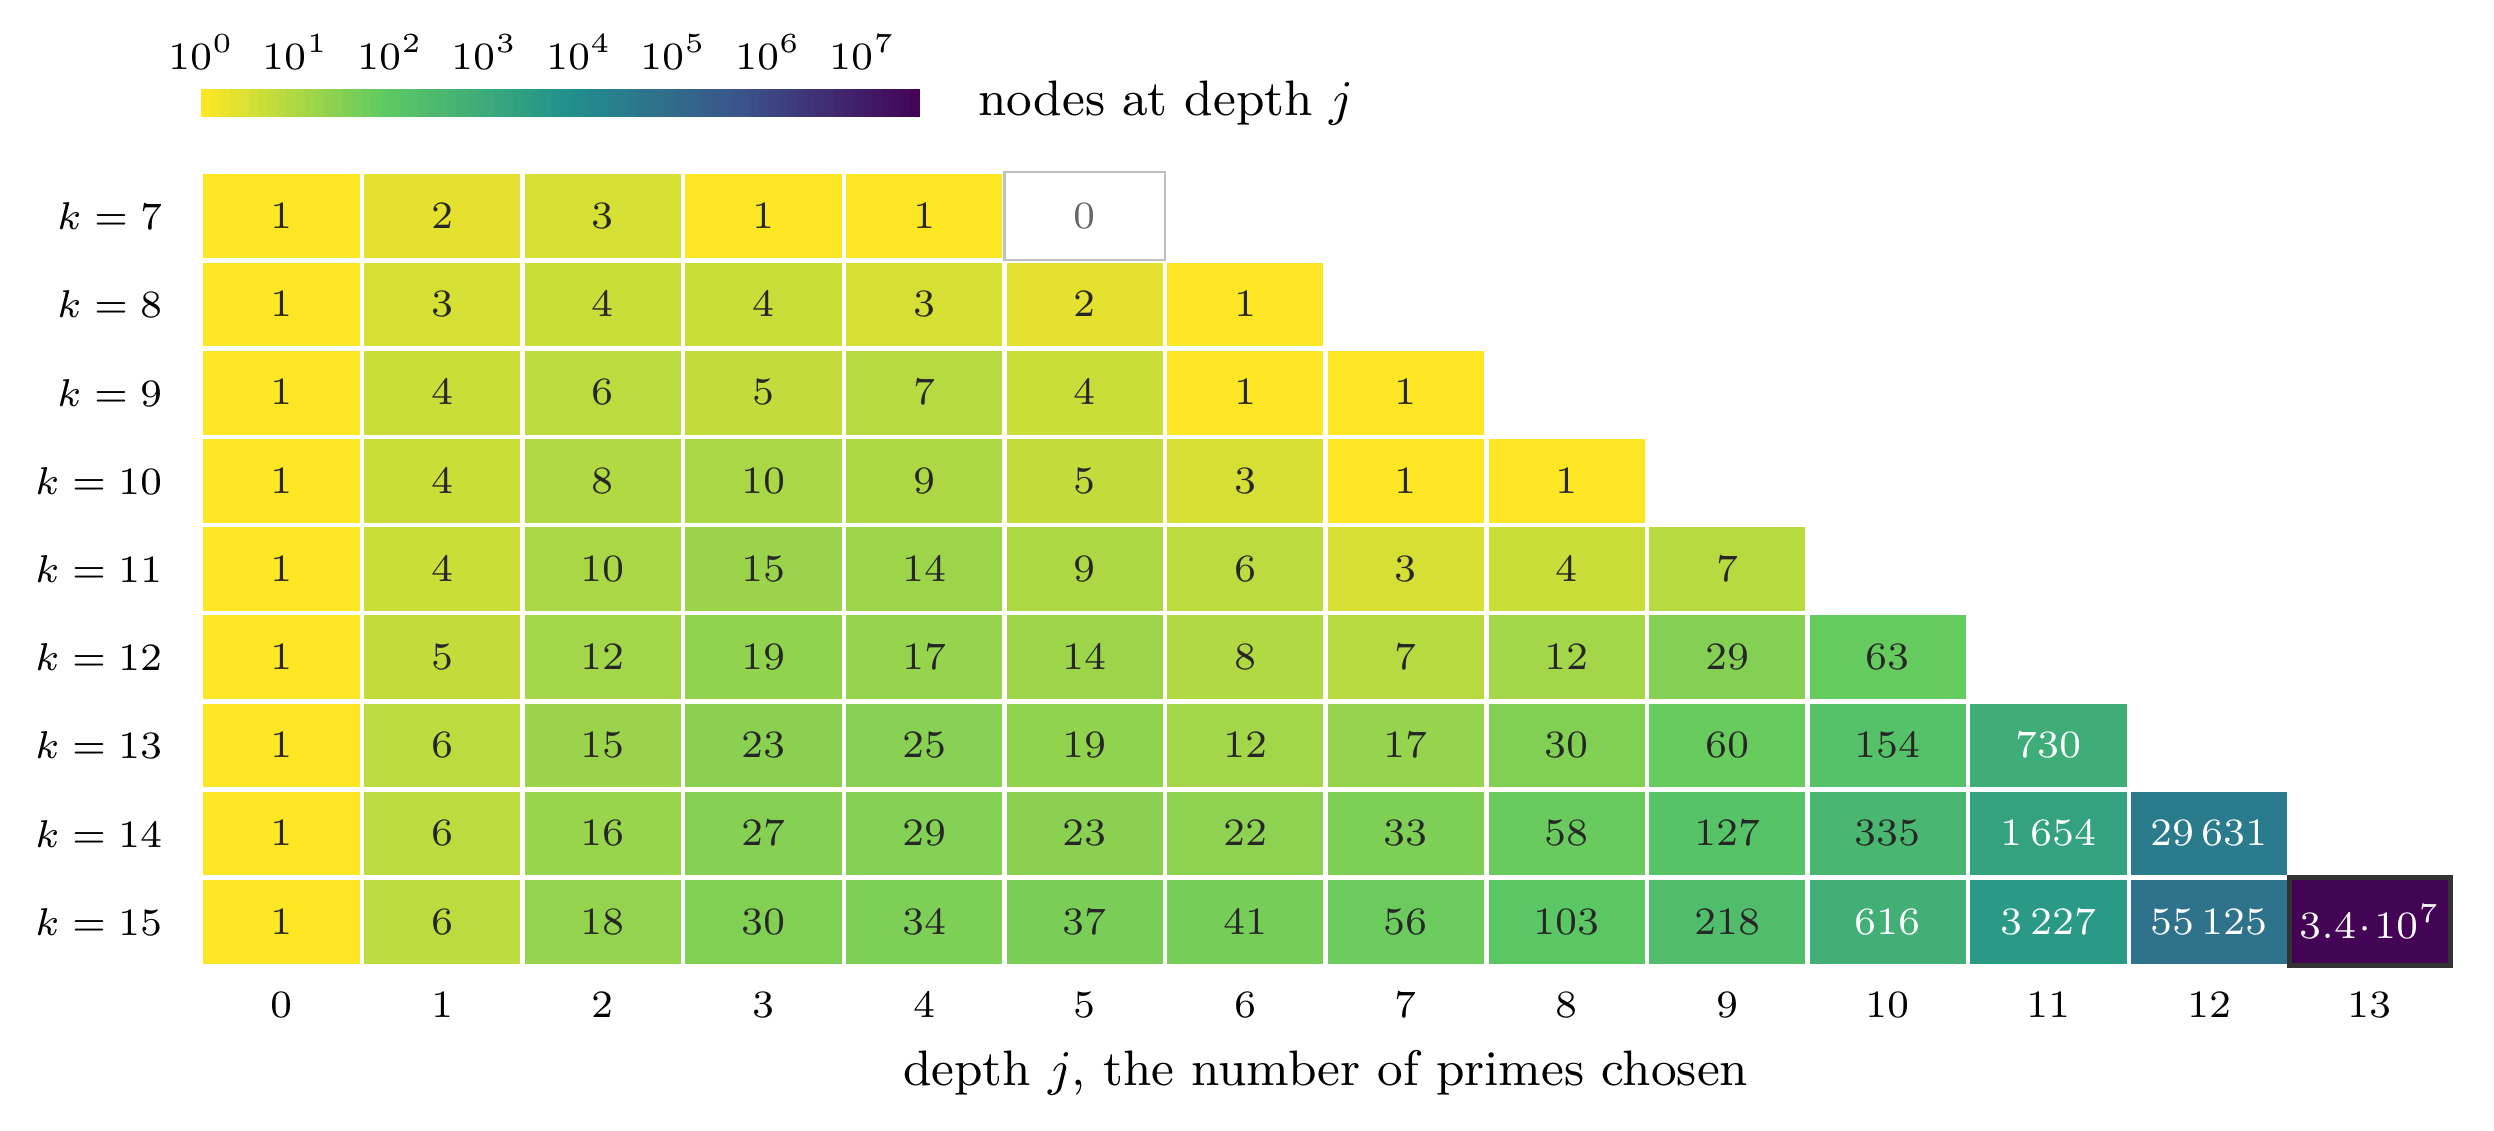
\includegraphics[width=\textwidth]{figures/fig_profile.png}
\caption{Number of nodes at each depth $j$ of the search for
$k=7,\dots,15$ primes, with the colour on a logarithmic scale. The
counts are the same for $n-1=2\varphi(n)$ and $n+1=2\varphi(n)$ with
$p_1\ge5$. The tree stays small until the last two levels. The last
cell of each row counts the nodes at depth $k-2$: for $k\le14$ these
are the nodes where $p_{k-1}$ is enumerated, and for $k=15$ (framed)
they are the $33865004$ choices of $p_{13}$, each completed by the
method of Section~\ref{sec:three}.}
\label{fig:profile}
\end{figure}

\subsection{Fifteen primes}\label{sec:fifteen}
For $k=15$ the traversal of Section~\ref{sec:search} is stopped at
depth $12$. The numbers of nodes at depths $0,1,\dots,12$ are
\[
  1,\ 6,\ 18,\ 30,\ 34,\ 37,\ 41,\ 56,\ 103,\ 218,\ 616,\ 3227,\ 55125,
\]
and $54985$ of the nodes at depth $12$ have a non-empty interval for
$p_{13}$. Both implementations of Section~\ref{sec:checks} produce the
same $54985$ prefixes with the same intervals, and so do the bounds
for $\varepsilon=+1$. The intervals have total length
$1.005\cdot10^9$ and contain $33865004$ primes $s$ that pass the
congruence prune. For each of these pairs of a prefix and a prime
$s=p_{13}$ we solved the two-prime problem of
Proposition~\ref{prop:class}, in which $N$ has between $40$ and $58$
digits.

Figure~\ref{fig:k15} shows how the pairs are distributed according to
the ratio $c^3/N$, which by Section~\ref{sec:three} decides how hard
the two-prime problem is. For $33786783$ of them, all but $0.23$ per
cent, the modulus satisfies $c^3>N$, so that Lenstra's bound applies
and a few boxes suffice. The remaining $78221$ pairs come from values
of $s$ just above the lower end of long intervals, where
$c=C_{12}s-2B_{12}$ is small. The most extreme is the prefix ending in
$25867$ of Table~\ref{tab:hard}, whose first admissible $s$ gives
$c^3/N\approx2\cdot10^{-15}$. In $473$ cases the estimated number of
boxes exceeded our threshold and $N$ was factored completely. The
whole computation took $19$ minutes of processor time with the first
implementation and $45$ minutes with the second, which factored $N$ in
$1772$ cases. The route of Section~\ref{sec:sum}, which factors
nothing, took 13 minutes (Table~\ref{tab:k15}).

For none of the $33865004$ pairs does $N$ have a divisor in the class of
Proposition~\ref{prop:class} that yields integers $s<p<q$, and all
three computations agree on this. So there is
not even a completion by composite integers, and in particular no
solution with $k=15$. Together with the case $k\le14$ this proves
Theorem~\ref{thm:first}.

\begin{table}[ht]
\centering
\caption{The case $k=15$ of $n-1=2\varphi(n)$, by the two lattice
implementations of Section~\ref{sec:three} and the route of
Section~\ref{sec:sum}. The three agree on each of the $55443$ pieces
into which the work was divided.}
\label{tab:k15}
\smallskip
\begin{tabular}{@{}lrrr@{}}
\toprule
 & first & second & sums \\
\midrule
prefixes of twelve primes & $54\,985$ & $54\,985$ & $54\,985$ \\
admissible choices of $p_{13}$ & $33\,865\,004$ & $33\,865\,004$ & $33\,865\,004$ \\
boxes & $82\,882\,379$ & $61\,384\,414$ & -- \\
lattice points tested & $30\,664\,171$ & $25\,527\,573$ & -- \\
trial divisions & -- & -- & $116\,427\,765$ \\
square tests & -- & -- & $82\,568\,071$ \\
complete factorisations of $N$ & $473$ & $1\,772$ & $0$ \\
completions $s<p<q$ in integers & $0$ & $0$ & $0$ \\
processor time & 19 min & 45 min & 13 min \\
\bottomrule
\end{tabular}
\end{table}

\begin{figure}[t]
\centering
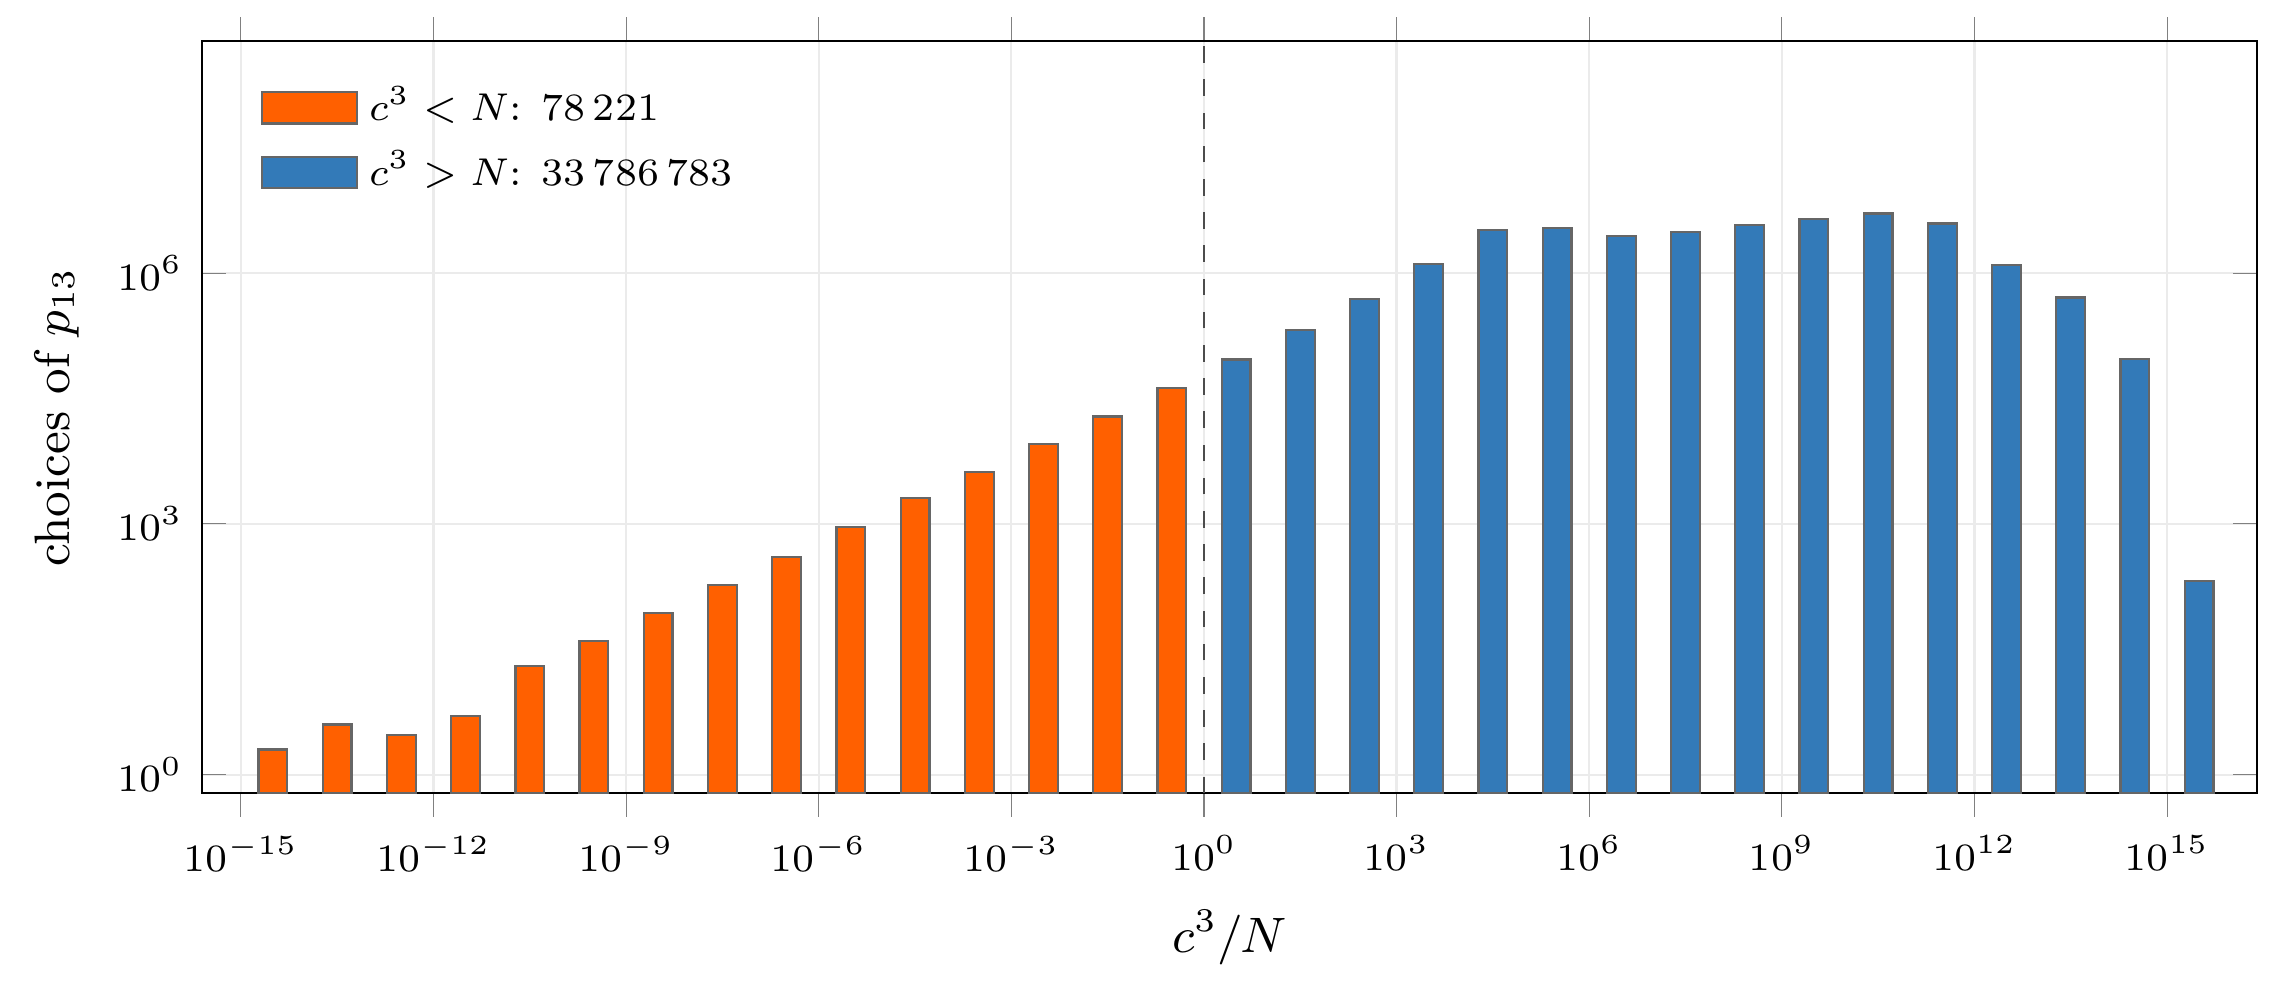
\includegraphics[width=0.92\textwidth]{figures/fig_k15.png}
\caption{The $33865004$ two-prime problems of the case $k=15$, by the
ratio $c^3/N$ on a logarithmic scale (bins of one decade). To the right
of the dashed line is Lenstra's range, where $N$ has at most $11$
divisors in the class and a few boxes find them. The left tail comes
from the lower ends of the longest intervals for $p_{13}$.}
\label{fig:k15}
\end{figure}

%%==================================================================
\section{The companion equation}\label{sec:second}
%%==================================================================

\subsection{Up to seven prime factors}\label{sec:seven}
Let $n$ satisfy \eqref{eq:second} with $\omega(n)\le7$. If $n\le3$
there is nothing to prove. Otherwise $n$ is odd, squarefree and
composite by Lemma~\ref{lem:basic}, and $n+1=2\varphi(n)$ by
Corollary~\ref{cor:seven}. Since $3$ may divide $n$, the search now
starts from $p_{\min}=3$, and we run it with $\varepsilon=+1$ for
$2\le k\le7$. The outcome is in Table~\ref{tab:seven}.

\begin{table}[ht]
\centering
\caption{The search for $n+1=2\varphi(n)$ with $3\le p_1$ and $k\le7$.}
\label{tab:seven}
\smallskip
\begin{tabular}{@{}rrrrl@{}}
\toprule
$k$ & nodes & terminal & largest width for $p_{k-1}$ & solutions found \\
\midrule
2 &     1 &     1 &                 1 & $15$ \\
3 &     3 &     2 &                 2 & $255$ \\
4 &     5 &     2 &                15 & $65535$ \\
5 &    11 &     4 &               256 & $83623935$, $4294967295$ \\
6 &    60 &    44 &            65\,536 & $6992962672132095$ \\
7 & 6\,914 & 6\,826 &          $2^{32}$ & none \\
\bottomrule
\end{tabular}
\end{table}

For $k\le6$ the search returns exactly the known solutions, each at
its own depth, and this is also a test of the programs. For $k=7$ it
returns nothing. Here the enumeration route is too slow, because one
terminal node, the prefix $3,5,17,257,65537$, has an interval for
$p_6$ of width $2^{32}$; for this prefix $C=1$ and
$D=2AB+C=2^{64}-2^{32}+1$, which is prime\footnote{Indeed
$A=2^{32}-1$, $B=2^{31}$ and $C=2B-A=1$, so
$D=2^{32}(2^{32}-1)+1=\Phi_6(2^{32})$, the sixth cyclotomic polynomial
at $2^{32}$. Its primality is well known and is confirmed by a
deterministic test, since $D<3.3\cdot10^{24}$.}. We
therefore use the divisor route throughout, which is rigorous in this
range: the largest integer $D$ factored in the case $k\le7$ has $21$
digits, so every factorisation is certified. For $k\le6$ the
enumeration route was also run and agrees node for node. This proves
Theorem~\ref{thm:eight} for solutions with at most seven prime
factors; the case of eight is treated in Section~\ref{sec:eight}.

\subsection{Solutions prime to three}
Let $n>3$ satisfy \eqref{eq:second} with $3\nmid n$ and
$\omega(n)\le15$. Then $n=p_1\cdots p_k$ with $5\le p_1$, and
$n+1=2\varphi(n)$ by Lemma~\ref{lem:Mtwo}. For $k\le6$ the product
$\prod p_i/(p_i-1)$ is at most $1.9490\ldots$, whereas
\eqref{eq:excess} requires it to be $2-1/\varphi(n)>1.99$. For
$7\le k\le14$ we ran both implementations with $\varepsilon=+1$ and
$p_{\min}=5$. Neither found a solution, and the node counts, the
numbers of terminal nodes and the largest widths coincide with those
of Table~\ref{tab:first} for every $k$. For $k=15$ the nodes at depth
$12$ and their intervals are again those of
Section~\ref{sec:fifteen}, and the method of Section~\ref{sec:three},
run with $\varepsilon=+1$ by both implementations and by the route of
Section~\ref{sec:sum} over the same $33865004$ pairs, finds no
completion in integers. This proves
Theorem~\ref{thm:coprime}.

The coincidence with Table~\ref{tab:first} has a simple cause. The
two sets of bounds in \eqref{eq:bounds} differ only by the terms
$1/(A_jW)$, which in this range are far smaller than the gaps between
consecutive admissible values of $p/(p-1)$ near the endpoints, and the
computation confirms that no endpoint moves. The tests
\eqref{eq:last} at the last level do differ, but by then the tree is
fixed. In this range, then, removing the prime $3$ makes
the two equations of Lehmer equally hard.

\subsection{Extensions of Fermat-type solutions}

\begin{proof}[Proof of Theorem~\ref{thm:ext}]
Let $2\varphi(n_0)=n_0+1$ and let $Q>1$ be squarefree and coprime to
$n_0$. Then $n=n_0Q$ satisfies $2\varphi(n)=n+1$ if and only if
$2\varphi(n_0)\varphi(Q)=n_0Q+1$, that is,
$(n_0+1)\varphi(Q)=n_0Q+1$, or
\begin{equation}\label{eq:ext}
  n_0\bigl(Q-\varphi(Q)\bigr)=\varphi(Q)-1 .
\end{equation}

(i) For $Q=q$ prime, \eqref{eq:ext} reads $n_0=q-2$.

(ii) For $Q=pq$ with primes $p<q$ we have $Q-\varphi(Q)=p+q-1$ and
$\varphi(Q)-1=pq-p-q$, so \eqref{eq:ext} becomes
$pq-(n_0+1)(p+q)+n_0=0$, and adding $(n_0+1)^2-n_0$ to both sides gives
\[
  (p-n_0-1)(q-n_0-1)=n_0^2+n_0+1 .
\]
Both factors on the left are positive. If both were negative we would
have $2\le p<q\le n_0$, and the left-hand side would be at most
$(n_0-1)^2<n_0^2+n_0+1$. Conversely, a factorisation
$n_0^2+n_0+1=de$ with $d<e$ gives $p=n_0+1+d$ and $q=n_0+1+e$, and if
both are prime then $n_0pq$ is a Fermat-type solution; the conditions
$p,q\nmid n_0$ hold because $p,q>n_0$. The divisor $d=1$ gives
$p=n_0+2$ and $q=(n_0+1)^2+1=n_0(n_0+2)+2$, which is the composition
of two one-prime extensions.

(iii) Factoring $n_0^2+n_0+1$ and testing $n_0+2$ for each of the
eight numbers gives Table~\ref{tab:ext}. The one-prime extensions are
$1\to3\to15\to255\to65535\to4294967295$ and
$83623935\to6992962672132095$. The two-prime extensions are those
listed in the table, and the only one that is not a composition of
one-prime extensions is $255\to83623935$. Every extension of each of
the eight numbers is therefore again one of the eight, and each of them
is reached from $1$, so the eight numbers are exactly the closure of
$\{1\}$. The rows for $65535$, $83623935$, $4294967295$ and
$6992962672132095$ show where the chains stop. Every factor in
Table~\ref{tab:ext} is below $2^{64}$, where the primality tests we use
are proofs, and a test that declares a candidate $p$ or $q$ composite
is never wrong.
\end{proof}

\begin{table}[ht]
\centering
\caption{One- and two-prime extensions of the Fermat-type solutions.}
\label{tab:ext}
\smallskip
\footnotesize
\begin{tabular}{@{}rcl@{}}
\toprule
$n_0$ & $n_0+2$ prime & factorisation of $n_0^2+n_0+1$; two-prime extensions $(p,q)$ \\
\midrule
$1$ & yes & $3$;\ \ $(3,5)$ \\
$3$ & yes & $13$;\ \ $(5,17)$ \\
$15$ & yes & $241$;\ \ $(17,257)$ \\
$255$ & yes & $97\cdot673$;\ \ $(257,65537)$ and $(353,929)$ \\
$65535$ & yes & $193\cdot22253377$;\ \ none \\
$83623935$ & yes & $67\cdot180097\cdot579535339$;\ \ none \\
$4294967295$ & no & $2^{64}-2^{32}+1$, prime;\ \ none \\
$6992962672132095$ & no & $13\cdot37\cdot109\cdot30802180789\cdot30280941915943441$;\ \ none \\
\bottomrule
\end{tabular}
\end{table}

The chains stop for the following reasons. For $n_0=65535$ the trivial divisor
gives $p=65537$ and $q=2^{32}+1=641\cdot6700417$, which is Euler's
factorisation of $F_5$, and the divisor $193$ gives $p=65729$, a
prime, but $q=22318913=3037\cdot7349$. For $n_0=4294967295$ the
one-prime extension fails because $n_0+2=2^{32}+1$ is composite once
more. Figure~\ref{fig:hyperbola} shows the hyperbolas for $n_0=255$
and $n_0=65535$ with their lattice points.

\begin{figure}[t]
\centering
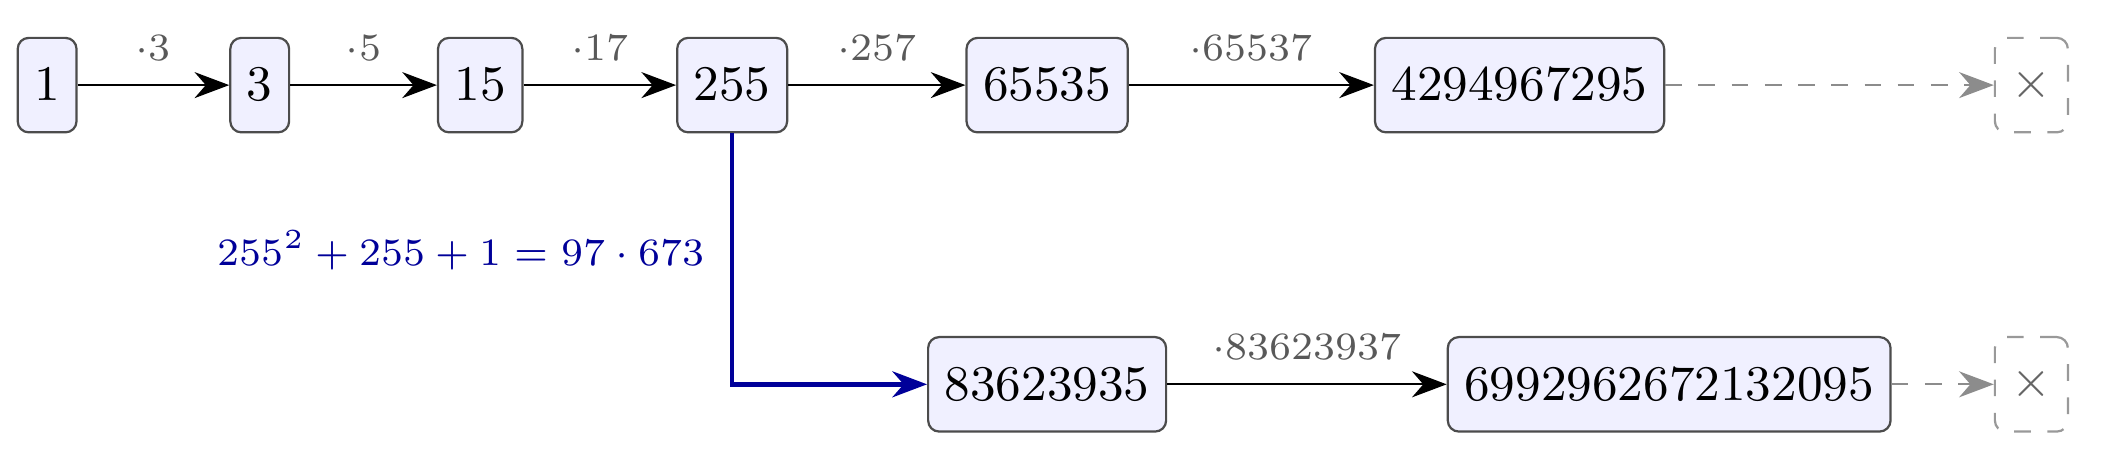
\includegraphics[width=0.84\textwidth]{figures/fig_tree.png}
\caption{The Fermat-type solutions of $n+1=2\varphi(n)$ as the closure
of $1$ under extensions. Horizontal arrows are one-prime extensions
$n_0\mapsto n_0(n_0+2)$, labelled by the prime $n_0+2$. The bent arrow
is the two-prime extension of $255$ by $(353,929)$, coming from the
factorisation $65281=97\cdot673$. Dashed arrows end the two chains:
$4294967297$ and $6992962672132097$ are composite, and neither
$n_0^2+n_0+1$ has a factorisation that yields two primes.}
\label{fig:tree}
\end{figure}

\begin{figure}[t]
\centering
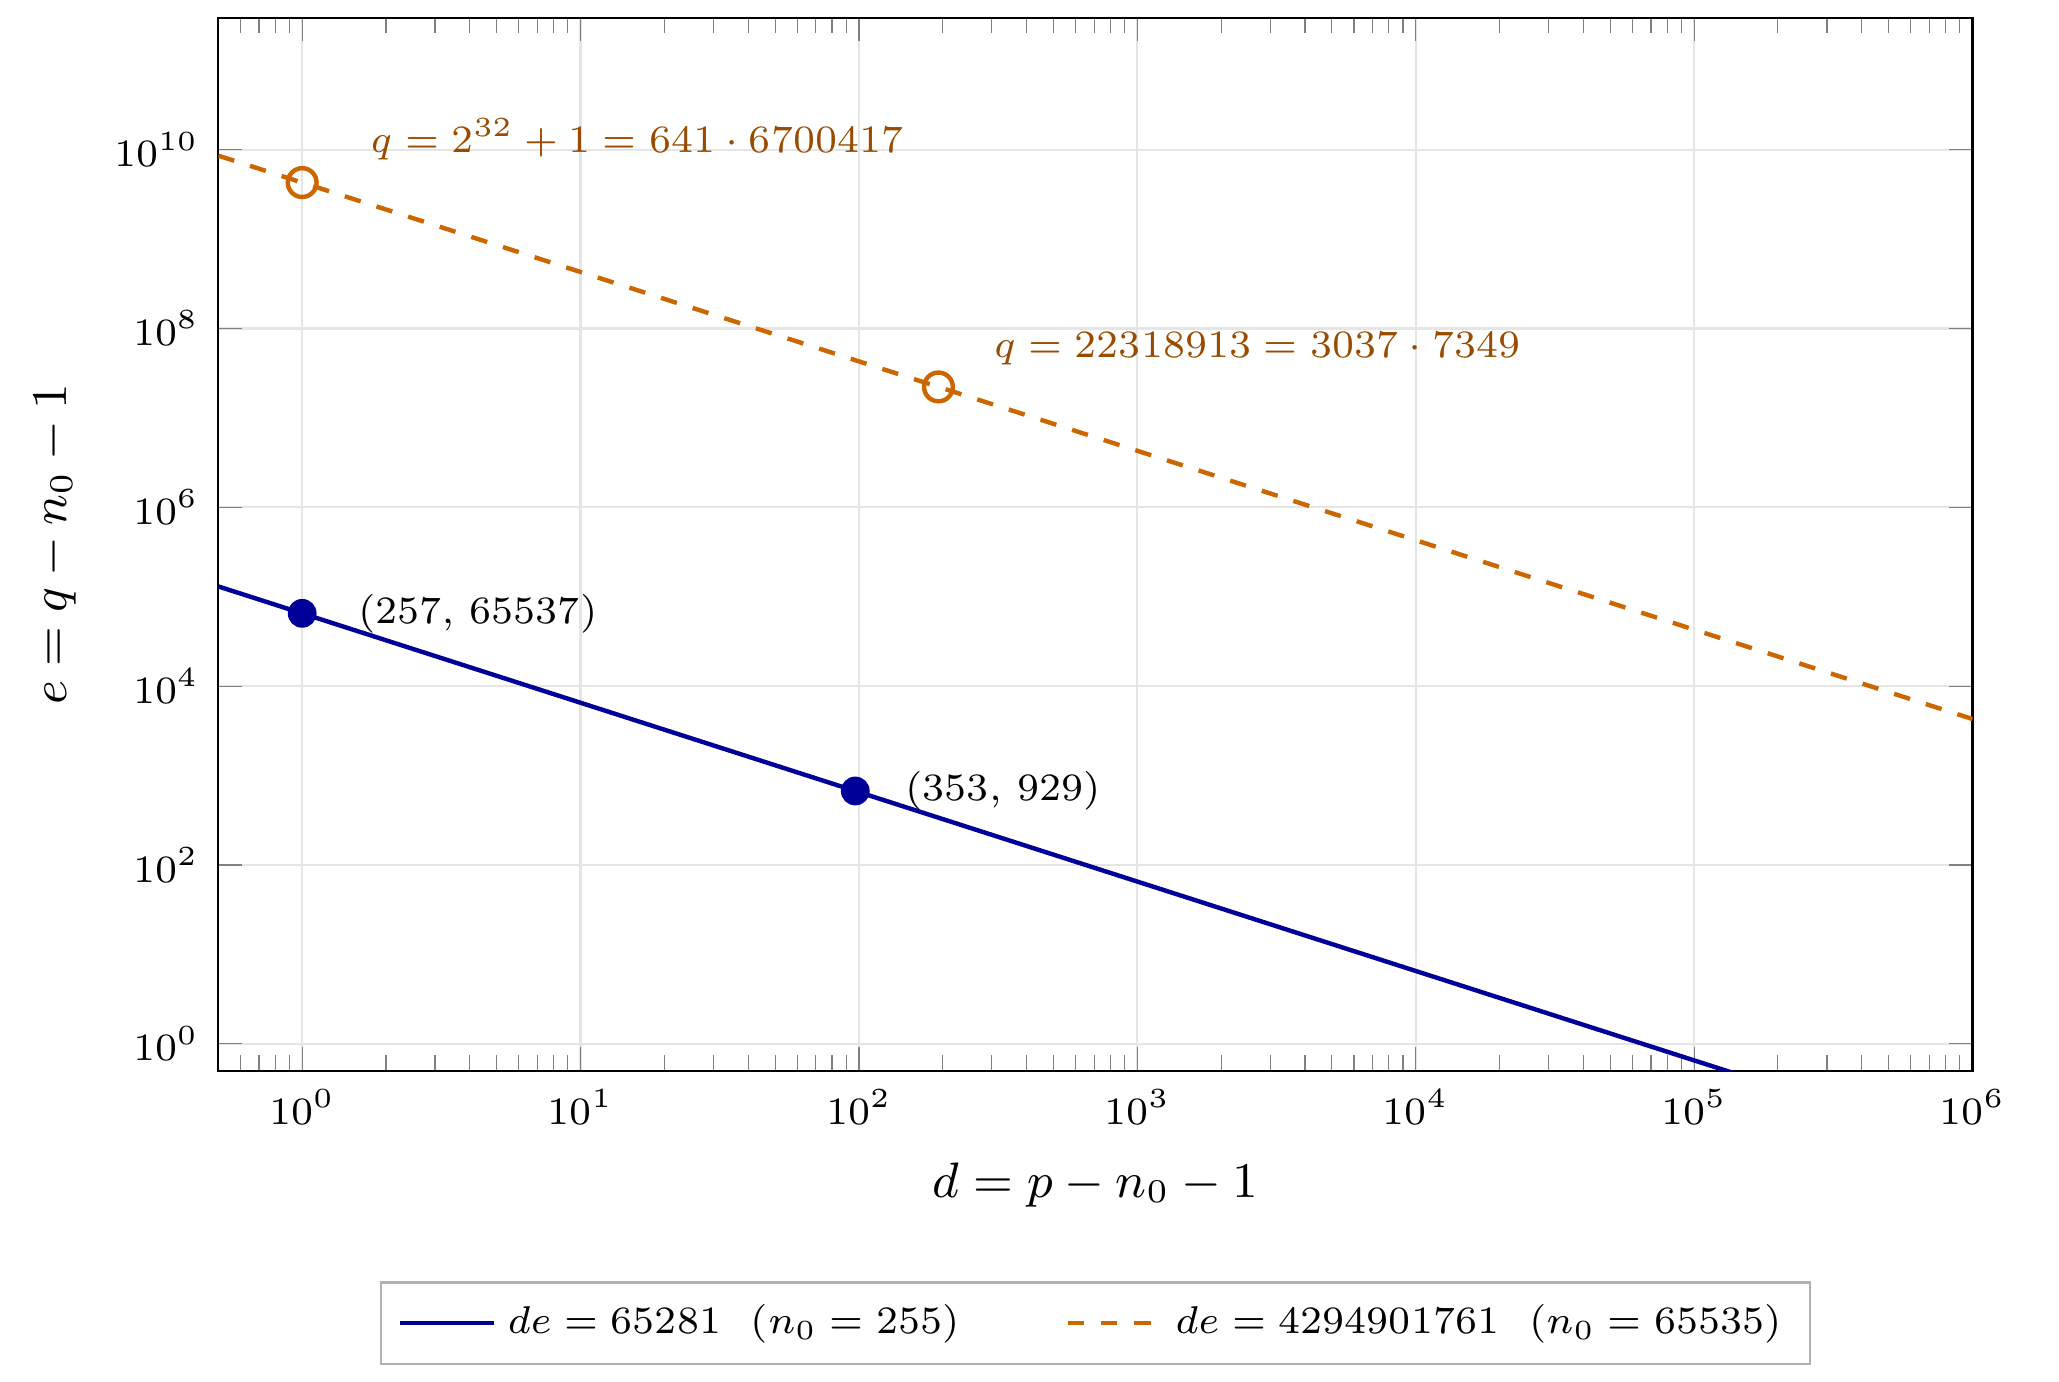
\includegraphics[width=0.82\textwidth]{figures/fig_hyperbola.png}
\caption{The two-prime extensions of $n_0$ are the lattice points
$(d,e)=(p-n_0-1,\,q-n_0-1)$ on $de=n_0^2+n_0+1$ with both $p$ and $q$
prime, shown on logarithmic axes. For $n_0=255$ both lattice points
with $d\le e$ give primes (filled). For $n_0=65535$ both lattice
points give a prime $p$ and a composite $q$ (open).}
\label{fig:hyperbola}
\end{figure}

\begin{remark}\label{rem:three}
For three new primes, $Q=spq$ with $s<p<q$, write $x=s-1$, $y=p-1$, $z=q-1$.
Equation \eqref{eq:ext} becomes
\[
  xyz=n_0\bigl(xy+yz+zx\bigr)+n_0(x+y+z)+n_0+1 ,
\]
and dividing by $n_0xyz$ shows that $1/x+1/y+1/z$ falls short of
$1/n_0$ by $\bigl(n_0(x+y+z)+n_0+1\bigr)/(n_0xyz)$, which is less than
$4/x^2$ because $x<y<z$. Hence $x$, the smallest of the three,
satisfies $3/x>1/n_0-4/x^2$ and $1/x<1/n_0$, that is,
$n_0<x<3n_0+2$. For
fixed $x$ the equation is bilinear in $y$ and $z$:
\[
  \bigl((x-n_0)y-n_0(x+1)\bigr)\bigl((x-n_0)z-n_0(x+1)\bigr)
  =(x-n_0)(n_0x+n_0+1)+n_0^2(x+1)^2 ,
\]
so the pair $(y,z)$ comes from the divisors of an integer of size about
$n_0^2x^2$. For $n_0=4294967295$ there are about $3.8\cdot10^8$
primes $s$ in the range, and $1.3\cdot10^8$ of them pass the
congruence prune: $s\equiv2\pmod3$ as Lemma~\ref{lem:three} requires,
and $s\not\equiv1$ modulo $5$, $17$, $257$ and $65537$. Each of them
leaves an integer of about forty digits to factor. This is the prefix $3,5,17,257,65537$ that
dominates the case $k=8$ in Section~\ref{sec:eight}.
\end{remark}

\subsection{Eight prime factors}\label{sec:eight}
Let $n$ satisfy \eqref{eq:second} with $\omega(n)=8$. Then $n>3$, and
$n$ is odd and squarefree by Lemma~\ref{lem:basic}. If $3\nmid n$, then
$\omega(n)\ge16$ by Theorem~\ref{thm:coprime}; hence $3\mid n$. By
Lemma~\ref{lem:three} the quotient $M$ is either $2$ or at least $5$,
and in the second case $\omega(n)\ge1540$. Hence $n+1=2\varphi(n)$ and
$p_1=3$, and it suffices to run the search with $\varepsilon=+1$ and
$k=8$ over the prefixes that begin with $3$.

The traversal down to depth $5$ takes a few seconds. It yields $10459$
prefixes $(p_1,\dots,p_5)$ with a non-empty interval for $p_6$, and
$10458$ of them begin with $3$. Their intervals have total length
$1.3045\cdot10^{10}$, and most of it belongs to a few prefixes
(Figure~\ref{fig:eight}, left): $8.59\cdot10^9$ to $3,5,17,257,65537$,
that is, to the solution $4294967295$ itself, where $C_5=1$;
$1.23\cdot10^9$ to $3,5,17,257,65543$; and $1.67\cdot10^8$ to
$3,5,17,353,929$, the solution $83623935$, where again $C_5=1$.
Thirty-four prefixes have an interval longer than $10^7$, and $326$
one longer than $10^6$. The intervals contain $228260561$ primes $s$ that
pass the congruence prune, $131788942$ of them for the prefix
$3,5,17,257,65537$. Each pair of a prefix and such a prime $s=p_6$
leaves the two-prime problem of Proposition~\ref{prop:class}, in which
$N$ has between $15$ and $40$ digits.

These problems lie far to the left of those of Figure~\ref{fig:k15}.
For the prefix $3,5,17,257,65537$ and $p_6=s$ one has
$A'=(2^{32}-1)s$ and $B'=2^{31}(s-1)$, so that the modulus is
$c=s-2^{32}$, and $N=2A'B'+c$ is close to $2^{64}s^2$. As $s$ runs
over $[2^{32}+1,\,3\cdot2^{32}-1]$, the ratio $c^3/N$ stays below
$2.1\cdot10^{-10}$, and the number $(N/c^3)^{1/2}$ that governs the
methods of Section~\ref{sec:three} grows from $7\cdot10^4$ at the
upper end to $4\cdot10^{16}$ at the first admissible prime,
$s=4294967357$, where $c=61$. We therefore combine the sum route with
trial division and with a complete factorisation, as follows.

Fix a prefix and an admissible prime $s$, define $A'$, $B'$, $c$, $N$
as in Section~\ref{sec:three}, and let $t=cp-2B'$ be the divisor of
Proposition~\ref{prop:class}. Since $p\ge s+2$, it satisfies
$t\ge t_0=c(s+2)-2B'$, and we choose a split point $t_d$ with
$t_0\le t_d$.
\begin{enumerate}[label=\textup{(\roman*)}, leftmargin=*]
\item The divisors with $t<t_d$ are found by running $p$ over the
  integers with $t_0\le cp-2B'<t_d$ and testing whether $t$ divides
  $A'p+\varepsilon$, as in Proposition~\ref{prop:last}. Since
  $c(A'p+\varepsilon)=A't+N$ and $\gcd(t,c)=1$ by
  Proposition~\ref{prop:class}, this is the same as testing whether $t$
  divides $N$, and the program does that when $A'p$ is too large for
  $128$-bit arithmetic.
\item For the divisors with $t_d\le t\le\sqrt N$ we use the sum
  $\sigma=p+q$ and the product $\pi=pq$. By \eqref{eq:hyperbola},
  \begin{equation}\label{eq:sigma}
    c\,\pi=2B'\sigma-2B'+\varepsilon,\qquad
    (q-p)^2=\sigma^2-4\pi ,
  \end{equation}
  so $\sigma$ lies in the class of $(2B'-\varepsilon)(2B')^{-1}$ modulo
  $c$, and $t+N/t=c\sigma-4B'$. As $x+N/x$ decreases on
  $(0,\sqrt N\,]$, the sum runs over its class in the range
  $2\sqrt N+4B'\le c\sigma\le t_d+N/t_d+4B'$, and each value is
  tested by asking whether $\sigma^2-4\pi$ is a perfect square. This
  is the route of Section~\ref{sec:sum}, written in terms of $p$ and
  $q$ instead of $u$ and $v$: the two sums differ by the constant
  $(2r+4B')/c$.
\item Both loops are sieved by congruences. Let $p<q$ be integers
  with $A'pq+1=2B'(p-1)(q-1)$. No $p_i$ divides $p-1$ or $q-1$, since
  it would then divide $1$. If moreover $p$ and $q$ have no prime
  factor up to $61$, which holds for primes larger than $s$ because
  every admissible $s$ exceeds $61$, then modulo every prime $\ell\le61$
  they avoid the residue $0$, and also the residue $1$ when $\ell$ is
  one of the $p_i$; in particular they are odd and congruent to $2$
  modulo $3$. Call these residues excluded. Since
  $X^2-\sigma X+\pi=(X-p)(X-q)$, the roots of this polynomial modulo a
  prime $\ell$ are $p$ and $q$ modulo $\ell$. The sieve discards only
  values of $\sigma$ that are odd, or not congruent to $1$ modulo $3$,
  or for which $\sigma^2-4\pi$ is not a square modulo one of $2^8$,
  $3^2$, $5^2$ and $7^2$, or for which, for some prime $\ell\le43$,
  the polynomial has no root modulo $\ell$ or a root at an excluded
  residue; and in the trial division it discards only values of $p$
  at an excluded residue modulo some prime $\ell\le61$. Every other
  value is tested exactly. So the sieve keeps every value that comes
  from integers $p$ and $q$ without prime factors up to $61$, and in
  particular every value that comes from primes.
\item If the estimated work of (i) and (ii) exceeds that of factoring
  $N$, about four milliseconds, then $N$ is factored completely with
  PARI/GP \cite{PARI}, every prime factor is proved
  prime,\footnote{With the option \texttt{factor\_proven} set, PARI/GP
  certifies every prime factor it returns. A factor below $2^{64}$ is
  certified by its Baillie--PSW test, which no composite number below
  $2^{64}$ passes; the PARI/GP documentation records that this was
  checked against the table of base-$2$ pseudoprimes below $2^{64}$ of
  Feitsma and Galway \cite{FG}. A larger factor is certified by the
  $n-1$ method \cite{BLS75} when enough of $n-1$ is known, and
  otherwise by the test of Adleman, Pomerance and Rumely
  \cite{APR83} in the form of Cohen and Lenstra \cite{CL84}.} and all
  divisors $t$ of $N$ with $t_0\le t\le\sqrt N$ in the class of
  Proposition~\ref{prop:class} are listed.
\end{enumerate}
Since $c$ is odd and prime to $3$, the admissible values of $\sigma$
form one class modulo $6c$. The work of (i) and (ii) is therefore about
$(t_d-t_0)/c$ values of $p$ and $(t_d+N/t_d-2\sqrt N)/(6c^2)$ values of
$\sigma$, and $t_d$ is chosen to minimise it (Figure~\ref{fig:routes}),
with the two kinds of steps weighted by their measured costs. With equal weights the minimum
lies near $t_d=(N/6c)^{1/2}$ and amounts to about $2(N/6c^3)^{1/2}$
steps, as in Section~\ref{sec:sum}. By the argument of that section,
(i) and (ii) together find every divisor $t\ge t_0$ of $N$ in the class
up to $\sqrt N$, and so does (iv); the sieve (iii) loses none that
comes from integers $p$ and $q$ without prime factors up to $61$. Where
$\sigma$ and $\pi$ are too large for $128$-bit arithmetic, (ii) is
carried out in multiprecision arithmetic. Now let $n$ be a solution with
$p_1=3$ and $k=8$. By Theorem~\ref{thm:complete} its first five primes
form one of the prefixes and $p_6$ is one of the admissible primes $s$
of its interval, and by Proposition~\ref{prop:class} its last two
primes give a divisor $t\ge t_0$ in the class. Hence $n$ is found.
Every completion $s<p<q$ in integers that is found is checked against
$A'pq+1=2B'(p-1)(q-1)$ exactly, and $p$ and $q$ are tested for
primality.

The computation was cut into $10897$ pieces, each a range of $s$
under one prefix, and run on four processors. It examined $228260561$
pairs, made $3.4\cdot10^{11}$ trial divisions, visited $6.7\cdot10^{13}$
values of $\sigma$ and tested $2.1\cdot10^{8}$ of them exactly.
In $1967265$ cases $N$ was factored, with up to $39$ digits. The
whole run took $6.9$ hours of processor time, $3.2$ of them in
PARI/GP. It found $21$ completions $s<p<q$ in integers and no
solution. Sixteen of the completions lie under the prefix
$3,5,17,353,929$ with $s=83623937$, where
$3\cdot5\cdot17\cdot353\cdot929\cdot s$ is the solution
$n_0=6992962672132095$. They are the pairs $p=n_0+1+d$, $q=n_0+1+e$ of
Theorem~\ref{thm:ext}(ii), one for each factorisation
$n_0^2+n_0+1=de$ with $d<e$, and by Table~\ref{tab:ext} none of them
consists of two primes. In each of the other five, listed in
Table~\ref{tab:eight}, $p$ or $q$ is divisible by one of
$p_1,\dots,p_5$. So \eqref{eq:second} has no solution with eight prime
factors, and
together with Section~\ref{sec:seven} this proves
Theorem~\ref{thm:eight}.

\begin{figure}[t]
\centering
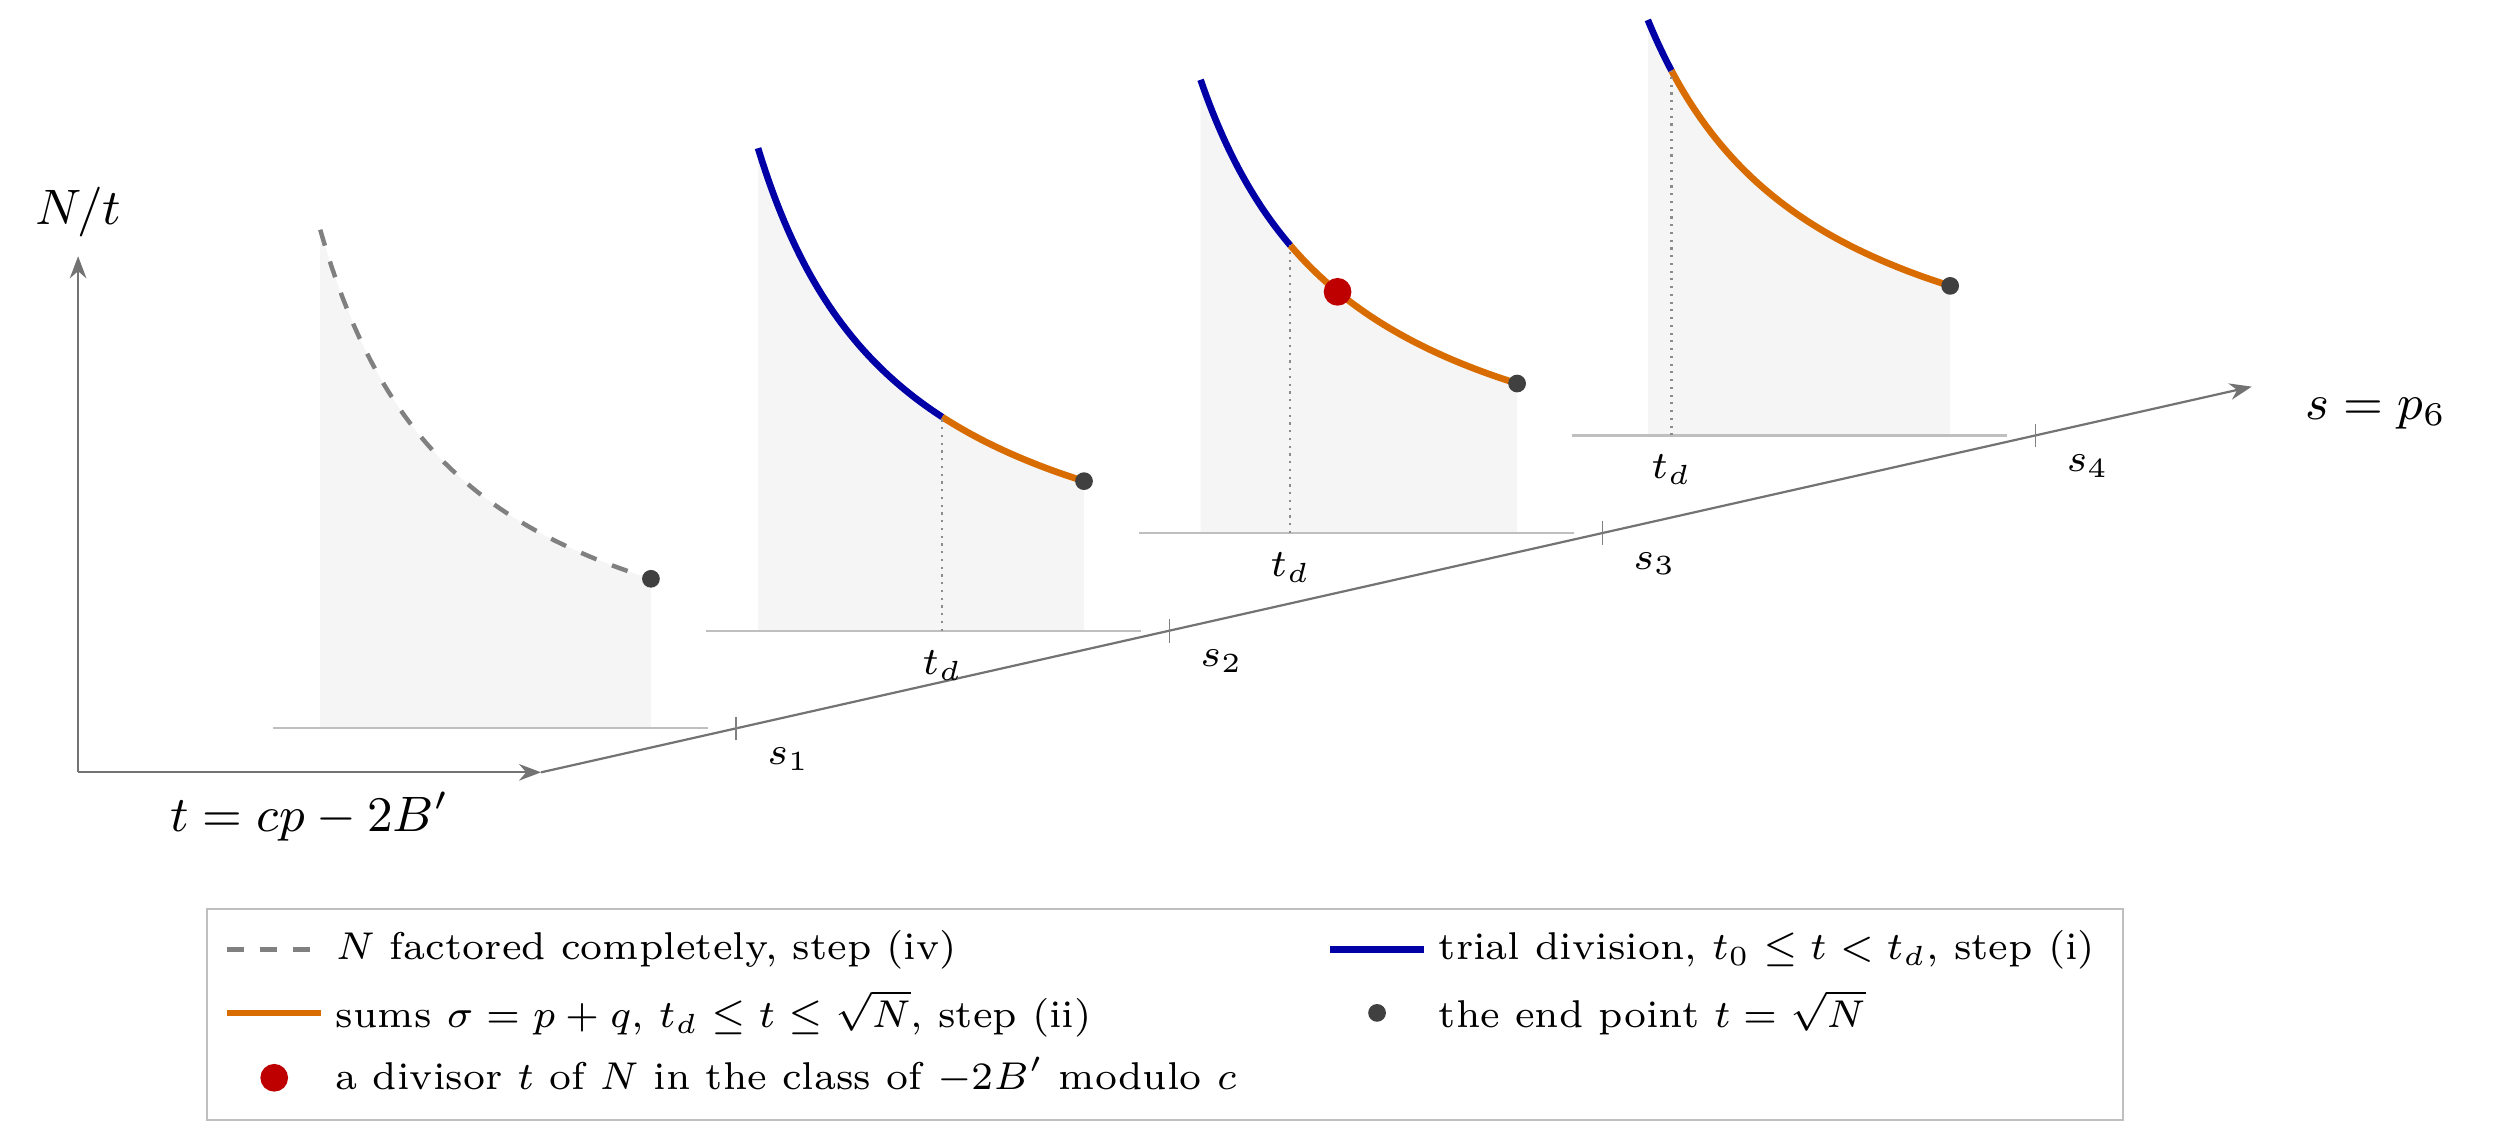
\includegraphics[width=\textwidth]{figures/fig_routes.png}
\caption{Steps (i), (ii) and (iv) for four admissible values
$s_1<s_2<s_3<s_4$ of $p_6$, not to scale. The divisors $t=cp-2B'$ of
$N$ with $t_0\le t\le\sqrt N$ lie on the branch $t\mapsto N/t$.
Trial division covers $t<t_d$ and the sums cover $t_d\le t\le\sqrt N$.
The split point $t_d$ is chosen for each $s$ to minimise the work, and
where both routes would be slow, as for $s_1$, the integer $N$ is
factored completely.}
\label{fig:routes}
\end{figure}

\begin{table}[ht]
\centering
\caption{The completions $s<p<q$ in integers of the case $k=8$ other
than the sixteen two-prime extensions of $6992962672132095$, with the
factorisations of $p$ and $q$.}
\label{tab:eight}
\smallskip
\footnotesize
\begin{tabular}{@{}lll@{}}
\toprule
$s=p_6$ & $p$ & $q$ \\
\midrule
\multicolumn{3}{@{}l}{prefix $3,5,17,257,65537$} \\
$4294967459$ & $17\cdot43\cdot673\cdot230521189693$ & $5\cdot409642859\cdot26363459459$ \\
$4294967969$ & $27419312914203719$ & $5\cdot19\cdot5011\cdot7699\cdot21393991009$ \\
$4596195557$ & $65533391633$ & $17\cdot20923232569978145771052877$ \\
\multicolumn{3}{@{}l}{prefix $3,5,17,353,929$} \\
$83625827$ & $3^2\cdot5^3\cdot13\cdot252862031$ & $3\cdot5\cdot7\cdot13\cdot113\cdot794656817253868193$ \\
$83760029$ & $3\cdot5\cdot3431155289$ & $3\cdot87389293\cdot45294677621$ \\
\bottomrule
\end{tabular}
\end{table}

\begin{figure}[t]
\centering
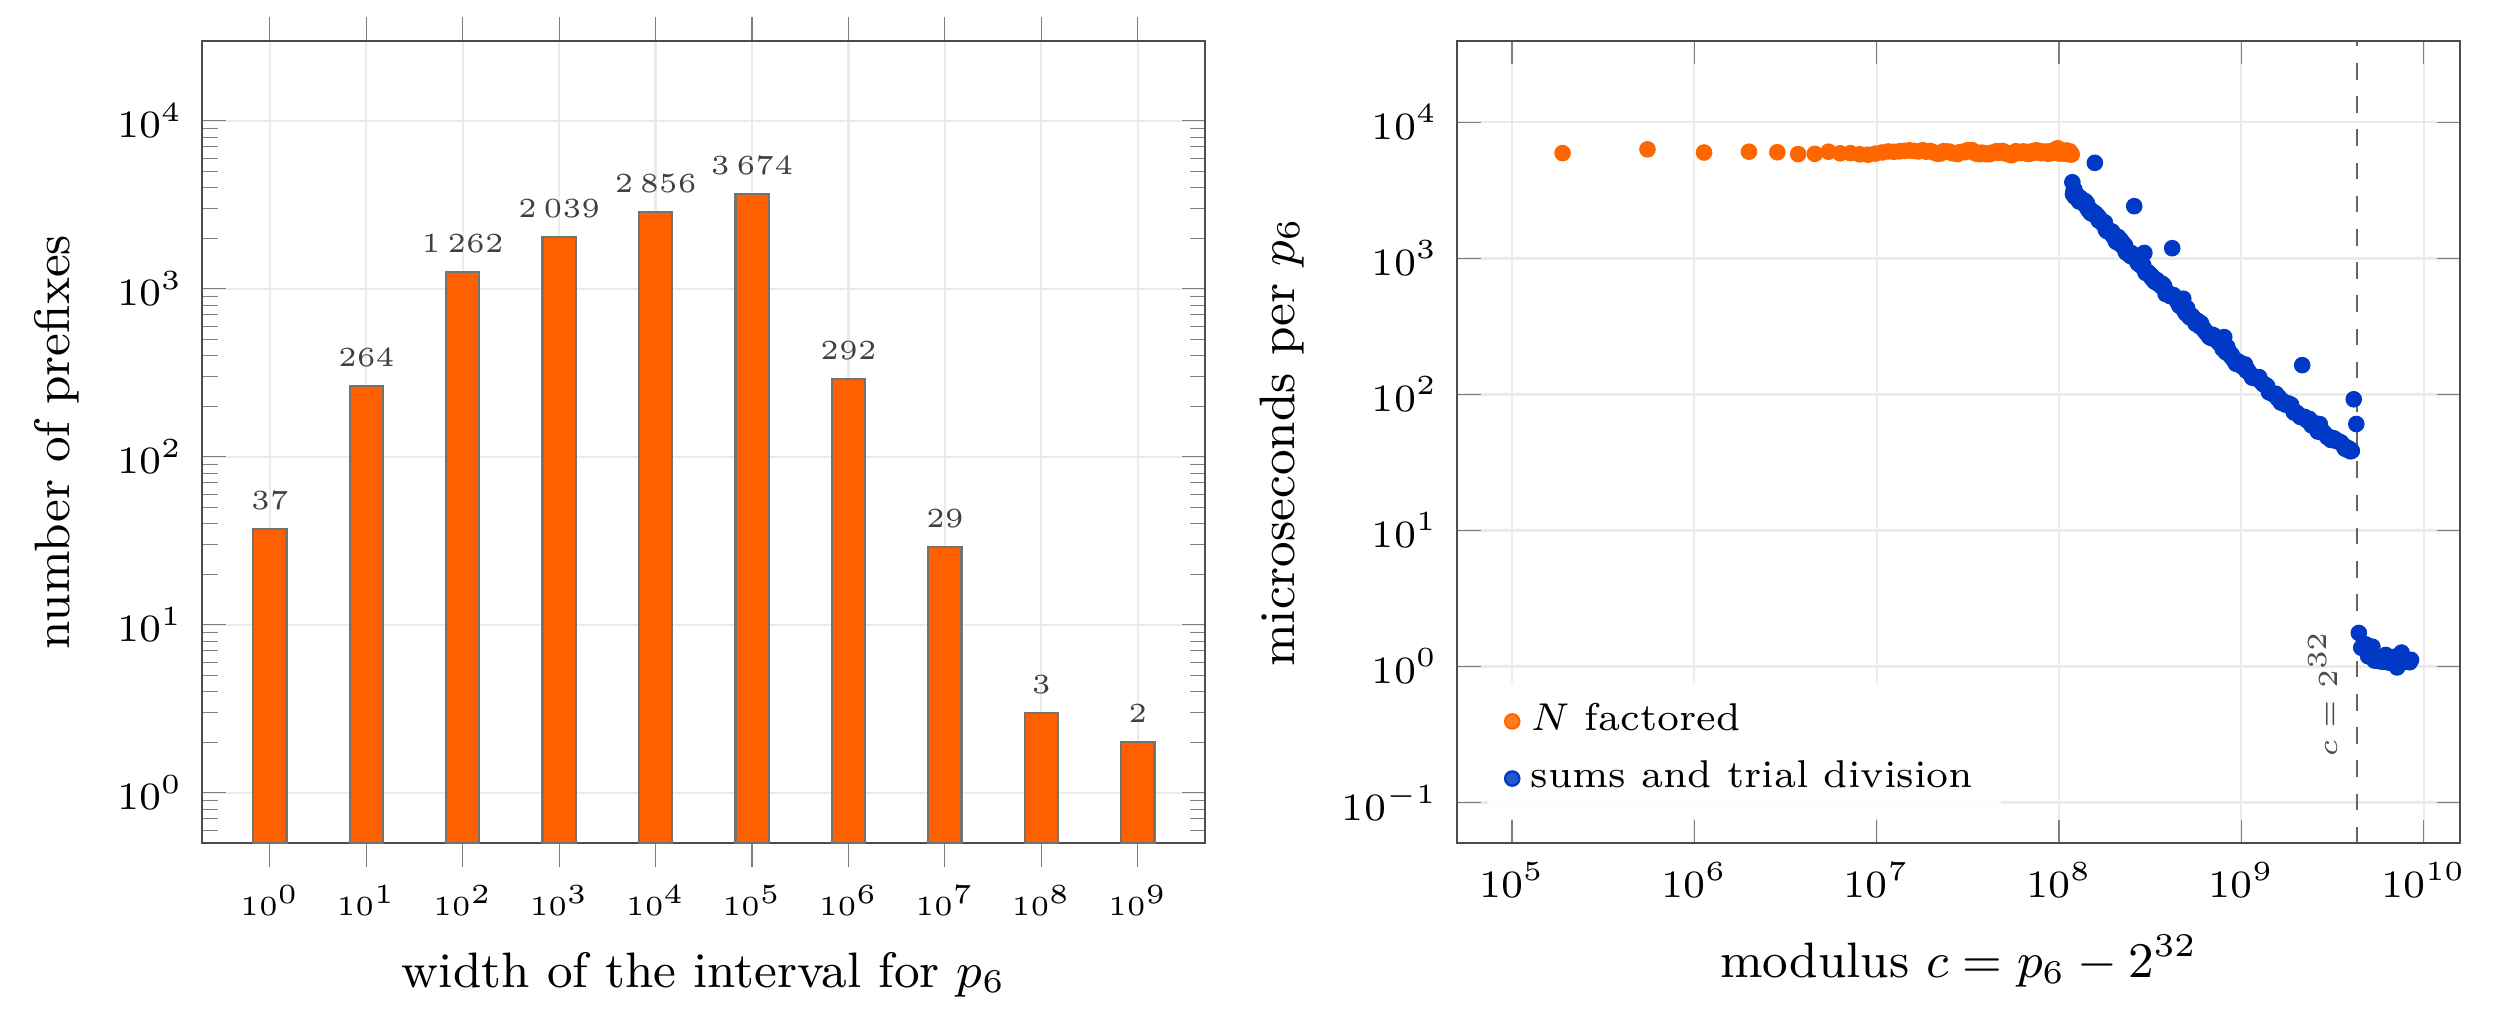
\includegraphics[width=\textwidth]{figures/fig_eight.png}
\caption{The case $k=8$ of the companion equation. Left: the
$10458$ prefixes $(3,p_2,\dots,p_5)$ by the width of the interval for
$p_6$, on logarithmic axes; the two in the last bar end in $65537$ and
$65543$. Right: processor time per admissible $p_6$ under the prefix
$3,5,17,257,65537$, one point for each piece of the run, against the
modulus $c=p_6-2^{32}$. For $c$ below about $10^8$ the integer $N$ is
factored, in about six milliseconds; above that the sums and the
trial division are faster, and their cost falls as $c$ grows. Beyond
$c=2^{32}$, that is for $p_6>2^{33}$, the condition $p>p_6$ leaves only
a short range of divisors.}
\label{fig:eight}
\end{figure}

%%==================================================================
\section{Checks on the computations}\label{sec:checks}
%%==================================================================

A search that finds nothing has to be tested on problems where there
is something to find, and it has to be implemented in more than one
way. We describe the checks we applied.

\subsection{Two implementations}
The first implementation is recursive and works with exact rational
arithmetic. At a terminal node it enumerates $p_{k-1}$ over its
interval when the interval is short or $D$ is large, and otherwise
enumerates the divisors of $D$. The second was written separately. It
traverses the tree iteratively with an explicit stack, works only with
the integers $A_j$ and $B_j$, computes the interval endpoints from a
floating-point guess corrected by integer comparisons, and at every
terminal node enumerates $p_{k-1}$ over the whole interval. It never
factors anything. For Theorems~\ref{thm:first} and \ref{thm:coprime}
the second implementation is the proof and the first a corroboration.
For Theorem~\ref{thm:eight} with $k=7$ the roles are reversed, for the
reason given in Section~\ref{sec:seven}, and the factorisations used
are all certified. In every run the two implementations visited the
same number of nodes. For $k=15$ the route of Section~\ref{sec:sum},
which factors nothing, plays the part of the second implementation,
and the two lattice implementations of Section~\ref{sec:three}
corroborate it. The case $k=8$ of Theorem~\ref{thm:eight} rests on
the program of Section~\ref{sec:eight}, whose checks are described in
Section~\ref{sec:checks8}.

\subsection{Equations with solutions}
Both implementations accept a general equation
\begin{equation}\label{eq:ab}
  b\,(n+\varepsilon)=a\,\varphi(n)
\end{equation}
with positive integers $a,b$, the bounds of
Section~\ref{sec:search} holding with $2$ replaced by $a/b$ and
\eqref{eq:hyperbola} becoming $(Cp-aB)(Cq-aB)=b(aAB+\varepsilon C)$
with $C=aB-bA$. For $\varepsilon=-1$, $b=2^k$ and $a=2^k+m$, equation
\eqref{eq:ab} says that $\prod_i(p_i-1)/2$ divides $n-1$ with quotient
$2^k+m$, and it has solutions. We ran both implementations with
$p_{\min}=3$ for $k=4$, $1\le m\le40$, and for $k=5$, $1\le m\le85$.
Both returned the same $56$ solutions, $20$ with $k=4$ and $36$ with
$k=5$, listed in Appendix~\ref{app:known}; each was verified by direct
arithmetic. The bounds and prunes exercised here are exactly those on
which Theorems~\ref{thm:first}--\ref{thm:coprime} depend.

\subsection{A sieve}
As a check that shares no code with the search, we computed
$\varphi(n)$ for all $n\le10^8$ by a sieve. There is no composite
$n\le10^8$ with $\varphi(n)\mid n-1$; the $n\le10^8$ with
$\varphi(n)\mid n+1$ are $1,2,3,15,255,65535,83623935$; and the odd
squarefree $n\le10^8$ with $\omega(n)\in\{4,5\}$ satisfying
\eqref{eq:ab} for the parameters above are exactly the ten members of
the list in Appendix~\ref{app:known} below $10^8$.

\subsection{The known solutions}
For $\varepsilon=+1$ and $p_{\min}=3$ the search is its own test:
Table~\ref{tab:seven} shows that every known Fermat-type solution with
at most six prime factors is found, at the right depth, and nothing
else.

\subsection{The last three primes}\label{sec:checks3}
The methods of Section~\ref{sec:three} were checked in five ways.

\emph{Brute force.} The routines that list the divisors of $N$ in a
residue class were compared with the list read off from a known
factorisation. The two lattice routines were run on $4000$ and $3674$
random integers $N$ of up to $93$ digits, with up to seven prime
factors of up to thirteen digits, some of them repeated. The moduli $c$
had between $2$ and $55$ per cent of the bits of $N$, so that $c^3/N$
ranged from about $10^{-82}$ to $10^{44}$, and the classes were chosen
at random or among the classes of actual divisors. Of these instances
$2764$ and $2586$ were handled by boxes, and the rest, where the
number of boxes would have exceeded the limit, by the factoring
fallback. The sum route was run on $3100$ integers
$N\equiv r^2\pmod c$ of up to $46$ digits, about half of them
products of two planted members of the class, with $c^3/N$ between
about $10^{-13}$ and $10^{28}$. All lists agreed.

\emph{Planted divisors.} We took $1400$ pairs of a prefix and a prime
$s$ from the search, $400$ of them just above the lower ends of the
forty longest intervals, where $c^3/N$ is smallest, and replaced $N$ by
the product of two members $t\le t^*$ of the class of about the same
size, with $t$ chosen log-uniformly; the values of $c^3/N$ ranged from
$10^{-7.7}$ to $10^{15}$. The sum route found the planted divisor in
all $1400$ cases. The lattice routines were run with factoring switched
off, a limit of $20000$ boxes and a limit of five seconds per instance.
They found the planted divisor in $1287$ and $1210$ cases and stopped
at a limit in the others. Nothing they returned was wrong, and whenever
two routines finished they returned the same list. The time limit is
needed because $r'=r$ makes the coset \eqref{eq:coset} a union of
lines $u+v=\text{const}$. A planted divisor puts a long segment of
such a line inside the box that contains it, and the lattice routines
examine every point of that segment. This affects only the running
time, and the runs of the search had no time limit.

\emph{Equations with solutions.} Used as a complete search from depth
$k-3$, both lattice implementations return the $56$ solutions of
\eqref{eq:ab} for $k=4$ and $k=5$. For \eqref{eq:second} with
$p_{\min}=3$ and $3\le k\le7$ they return exactly the solutions
$255$, $65535$, $83623935$, $4294967295$ and $6992962672132095$ of
Table~\ref{tab:seven}, and nothing with $k=7$. Since every
factorisation in these runs is certified, this re-derives the case
$3\le k\le7$ of Theorem~\ref{thm:eight} independently of
Section~\ref{sec:seven}. The sum route, applied to the first $k-2$
primes of each of these $61$ solutions, returns the solution. For
$7\le k\le14$ and both signs of $\varepsilon$ all three find no
solution, and the number of choices of $p_{k-2}$ they treat equals the
number of nodes at depth $k-2$ found in Sections~\ref{sec:first}
and~\ref{sec:second}.

\emph{The lattice route alone.} For each of the $61$ known solutions
we took $s=p_{k-2}$ from the solution and asked the first
implementation, with factoring switched off, for the divisors of $N$ in
the class. In all $36$ cases with $c>1$ the divisor $t=cp_{k-1}-aB'$
was among them; when $c=1$ every integer lies in the class and only
factoring applies. The second implementation assumes $\gcd(r,c)=1$,
which holds in the search by Proposition~\ref{prop:class} but in only
one of these cases, and there it found $t$ as well.

\emph{Agreement.} For each sign of $\varepsilon$ the three
computations divided the case $k=15$ into the same $55443$ tasks,
counted the same number of primes $p_{13}$ in every task, and returned
no completion in integers in any task.

\subsection{The eight-prime search}\label{sec:checks8}
The program of Section~\ref{sec:eight} was tested in four ways
before the runs, and part of the eight-prime run was repeated
afterwards.

\emph{Known solutions.} Run with prime entries, $\varepsilon=+1$ and
$p_{\min}=3$ from depth $k-3$ for $3\le k\le7$, the program returns
the solutions $255$, $65535$, $83623935$, $4294967295$ and
$6992962672132095$, and no other completion with prime entries. The
runs were repeated with every divisor sent to the trial division (i),
with every divisor sent to the sum route (ii), and with the
multiprecision arithmetic used for every quantity; all runs return the
same completions among those in which $p$ and $q$ have no prime factor
up to $61$ other than themselves.

\emph{Odd integers.} With the conditions modulo $3$ removed, and with
the congruence prune of Theorem~\ref{thm:pseudo3} in place of the
conditions on primes, the program solves \eqref{eq:product} in odd
integers. For $3\le k\le7$ it finds $1$, $1$, $2$, $8$ and $47$
solutions with $\varepsilon=-1$, and $1$, $1$, $2$, $4$ and $18$ with
$\varepsilon=+1$, the numbers found by the independent program of
Theorem~\ref{thm:pseudo3}, and again all runs agree.

\emph{Complete factorisation.} We took $400$ random pairs of a prefix
of the case $k=8$ and an admissible prime $s$, and all $2468$
admissible primes $s$ in three ranges under the prefix
$3,5,17,257,65537$: just above $2^{32}$, where $c$ is small and most
$N$ are factored; around $2^{33}$; and around $s=4596195557$, which
has a completion in integers. The completions found by the program,
together with those found by factoring the $633$ integers $N$ it
passed on to PARI/GP, coincide with those found by factoring $N$ for
every one of the $2868$ pairs. There are three of them, and they
reappear in Table~\ref{tab:eight}.

\emph{Thirteen entries.} The case $k=13$ of
Theorem~\ref{thm:pseudo3}(i) uses the program with odd entries prime
to $3$. For each sign we took $600$ values of $x_{11}$, $270$ of them
at nine places of the longest interval and $330$ under random nodes,
and compared the completions found by the program with those read off
from a complete factorisation of $N$, which has up to $55$ digits. The
two agree: for none of these values does $N$ have a divisor in the
class that yields integers $x_{11}<p<q$.

\emph{Repetition.} After the run, $13$ pieces chosen at random with a
fixed seed among the $441$ whose counts the run records separately,
and the
piece that contains the four completions in which $p$ and $q$ have no
prime factor up to $61$, were run again with other parameters. The
sums were weighted more than three times as heavily against the trial
division, so that the split points $t_d$ move, and $N$ was factored
whenever the estimated work exceeded $1.5$ milliseconds instead of
four. The repetition treated $7415547$ admissible values of $p_6$ and
factored $196063$ integers $N$. It found the same number of admissible
values of $p_6$ in each of the $13$ pieces as the run, and the same
four completions.

\subsection{Formal verification}\label{sec:lean}
The statements listed in Table~\ref{tab:lean} have been proved in
Lean~4 \cite{Lean4}, version~4.34.1, using Mathlib \cite{Mathlib}. The
bounds of Proposition~\ref{prop:bounds} and the identities of
Propositions~\ref{prop:last} and~\ref{prop:class} are proved for
arbitrary integers $A,B,p,q$ satisfying the hypotheses used in the
text, so that they apply at every node of the search. Lemma~\ref{lem:firsthit}
is proved for the recursive function itself: the function terminates,
every value it returns is the least solution, and when it reports that
there is none, there is none. The kernel of Lean checks every proof,
and Lean reports that the theorems depend only on its three standard
axioms, namely propositional extensionality, choice and the soundness
of quotients. No statement is assumed without proof, and no step is
delegated to compiled code.\footnote{Finite checks are made by kernel
reduction of decidable propositions. The alternative that evaluates
such propositions by compiled code, and would add an axiom trusting
the compiler, is not used.}

The proofs of Lemmas~\ref{lem:three}, \ref{lem:Mtwo} and
Corollary~\ref{cor:seven} need the first $1538$ primes congruent to $2$
modulo $3$ from $5$ on, the first $32$ primes from $5$ on, and the
odd primes up to $19$, and they need to know that no prime is missing
from these lists. The formal proof walks through the arithmetic
progression $5,11,17,\dots$ (respectively the odd numbers) and checks
a prime divisor for each member left out of the list; it then
evaluates the products of $p/(p-1)$ in exact arithmetic. For
Theorem~\ref{thm:ext}(iii) it checks the factorisations of
Table~\ref{tab:ext}, proves each prime that occurs there prime, by
trial division below $10^7$ and above $10^7$ by Lucas's converse of
Fermat's theorem,\footnote{If $a^{p-1}\equiv1\pmod p$ and
$a^{(p-1)/\ell}\not\equiv1\pmod p$ for every prime $\ell\mid p-1$, then
$a$ has order $p-1$ modulo $p$, and so $p$ is prime. The certificate
for $p$ consists of $a$ and the factorisation of $p-1$, whose prime
factors are certified in the same way. The seven primes certified like
this range from $22253377$ to $2^{64}-2^{32}+1$.} and proves each
composite candidate composite by exhibiting a divisor.

For the case of eight prime factors the formal proofs cover the
reduction to $n+1=2\varphi(n)$ and $p_1=3$, which takes
Theorem~\ref{thm:coprime} as its hypothesis $3\mid n$; the identity
$c(A'p+\varepsilon)=A't+N$ and the equivalence of the two divisibility
tests in step (i); equation \eqref{eq:sigma}, the class and the range
of $\sigma$, and the converse that turns a square value of
$\sigma^2-4\pi$ back into a pair $p,q$ in step (ii); and step (iii) in
the form that the sieve keeps every value coming from integers $p$ and
$q$ at no excluded residue. The two facts that supply this hypothesis
are proved as well: integers without prime factors up to $61$ avoid
the excluded residues of the eight-prime search, and every completion
in odd integers prime to $3$ avoids those of the search for $k=13$ in
Theorem~\ref{thm:pseudo3}. The kernel checks each of the $21$
completions $s<p<q$: it verifies the equation and a proper divisor of
$p$ or of $q$. The
exhaustive searches of Sections~\ref{sec:first} and~\ref{sec:second}
and the completeness statements Theorems~\ref{thm:complete}
and~\ref{thm:three}, which concern the programs, are not formalised,
and neither are the searches behind Theorem~\ref{thm:pseudo3}. The
proof of Theorem~\ref{thm:pseudo25} is formalised in full: the kernel
checks the tuple with $25$ entries, and the two extension steps are
proved for arbitrary tuples.

\begin{table}[ht]
\centering
\caption{The statements verified in Lean.}
\label{tab:lean}
\smallskip
\small
\begin{tabular}{@{}ll@{}}
\toprule
statement & extent \\
\midrule
Lemmas~\ref{lem:basic}, \ref{lem:three}, \ref{lem:Mtwo}, Corollary~\ref{cor:seven} & in full, with the thresholds $1540$, $32$, $7$ \\
Theorem~\ref{thm:quotient} & in full \\
Propositions~\ref{prop:below2}, \ref{prop:bounds} & in full \\
Proposition~\ref{prop:last} & in full, with its converse \\
Proposition~\ref{prop:class} & in full, with $\gcd(r,c)=1$ from the prune \\
Lemmas~\ref{lem:box}, \ref{lem:firsthit} & in full \\
Section~\ref{sec:sum} & identity \eqref{eq:sum}, its converse, the bound $c^3<N+2c^2$ \\
Theorem~\ref{thm:ext} & (i), (ii) and (iii) in full \\
Remark~\ref{rem:three} & both identities \\
Proposition~\ref{prop:pseudo} & in full \\
Lemma~\ref{lem:parity} & in full, with $\gcd(x_i,x_j-1)=1$ from \eqref{eq:product} \\
Proposition~\ref{prop:local} & in full \\
Theorem~\ref{thm:pseudo25} & in full, the tuple checked by the kernel \\
Proposition~\ref{prop:lehmerext} & in full, quadratic reciprocity from Mathlib \\
Section~\ref{sec:eight} & reduction, steps (i)--(iii), the $21$ completions \\
Theorem~\ref{thm:pseudo3}, $k=13$ & the sieve keeps every completion \\
\bottomrule
\end{tabular}
\end{table}

%%==================================================================
\section{The next cases}\label{sec:walls}
%%==================================================================

The methods of Section~\ref{sec:three} settle the case $k=15$ in a
quarter of an hour on a single processor, and the case of eight primes
of the companion equation in $6.9$ hours. This section explains why
they do not reach the next cases, and which properties of the primes
any further progress has to use.

\subsection{Lehmer's equation with sixteen primes}
For $k=16$ the traversal down to depth $12$ is again a matter of
seconds. It produces $90092$ prefixes with four primes still to
choose, and their intervals for $p_{13}$ have total length
$1.6\cdot10^9$ (Figure~\ref{fig:walls}). They contain
$1.2\cdot10^8$ primes, of which $5.4\cdot10^7$ pass the congruence
prune. The widest interval, of length $1.6\cdot10^8$, belongs once
more to the prefix ending in $25867$. Each admissible $p_{13}$ now
leaves three primes to choose, and every admissible $p_{14}$ then
leaves a two-prime problem of the kind solved in
Section~\ref{sec:three}. Near the lower end of a long interval the shortfall
$C_{13}/A_{13}$ after $p_{13}$ is tiny, so the interval for $p_{14}$
is very long. If $T-1$ is the shortfall after twelve primes, and $x_0$
is about $1/(T-1)$, a choice $p_{13}=x_0+d$ leaves a shortfall of about
$(T-1)^2d$ and hence an interval of length about
$2/\bigl((T-1)^2d\bigr)$ for $p_{14}$. Summing over the admissible
primes $p_{13}$, and counting the primes $p_{14}$ with density
$1/\log x$ and the share of them that passes the prune, gives to first
order some $4\cdot10^{14}$ pairs of primes $(p_{13},p_{14})$, of which
about $9\cdot10^{13}$ are admissible, two thirds of these from the
single prefix ending in $25867$, where $T-1=1.8\cdot10^{-8}$. The integers $N$ of the resulting two-prime problems are as large as
$10^{86}$, and about $10^{77}$ on average. At the average speed of the sum route for
$k=15$, $24$ microseconds per problem, the admissible pairs alone
would take $2\cdot10^9$ processor seconds. The problems with a small
modulus add to this. Close to the lower end of each interval for $p_{14}$
the modulus $c$ is small: about eleven per cent of the problems have
$c^3<N$, where the work grows like $(N/c^3)^{1/2}$, some $10^9$ have
$c^3/N<10^{-12}$, and for the smallest $c$ the integer $N$ would have
to be factored. With these the total is of the order of $10^{10}$
processor seconds, some three centuries. The case $k=16$ is therefore
far beyond a single machine. It would need a very large computation,
or better a new idea, for instance a way of treating a whole
range of $p_{13}$ at once.

\begin{figure}[t]
\centering
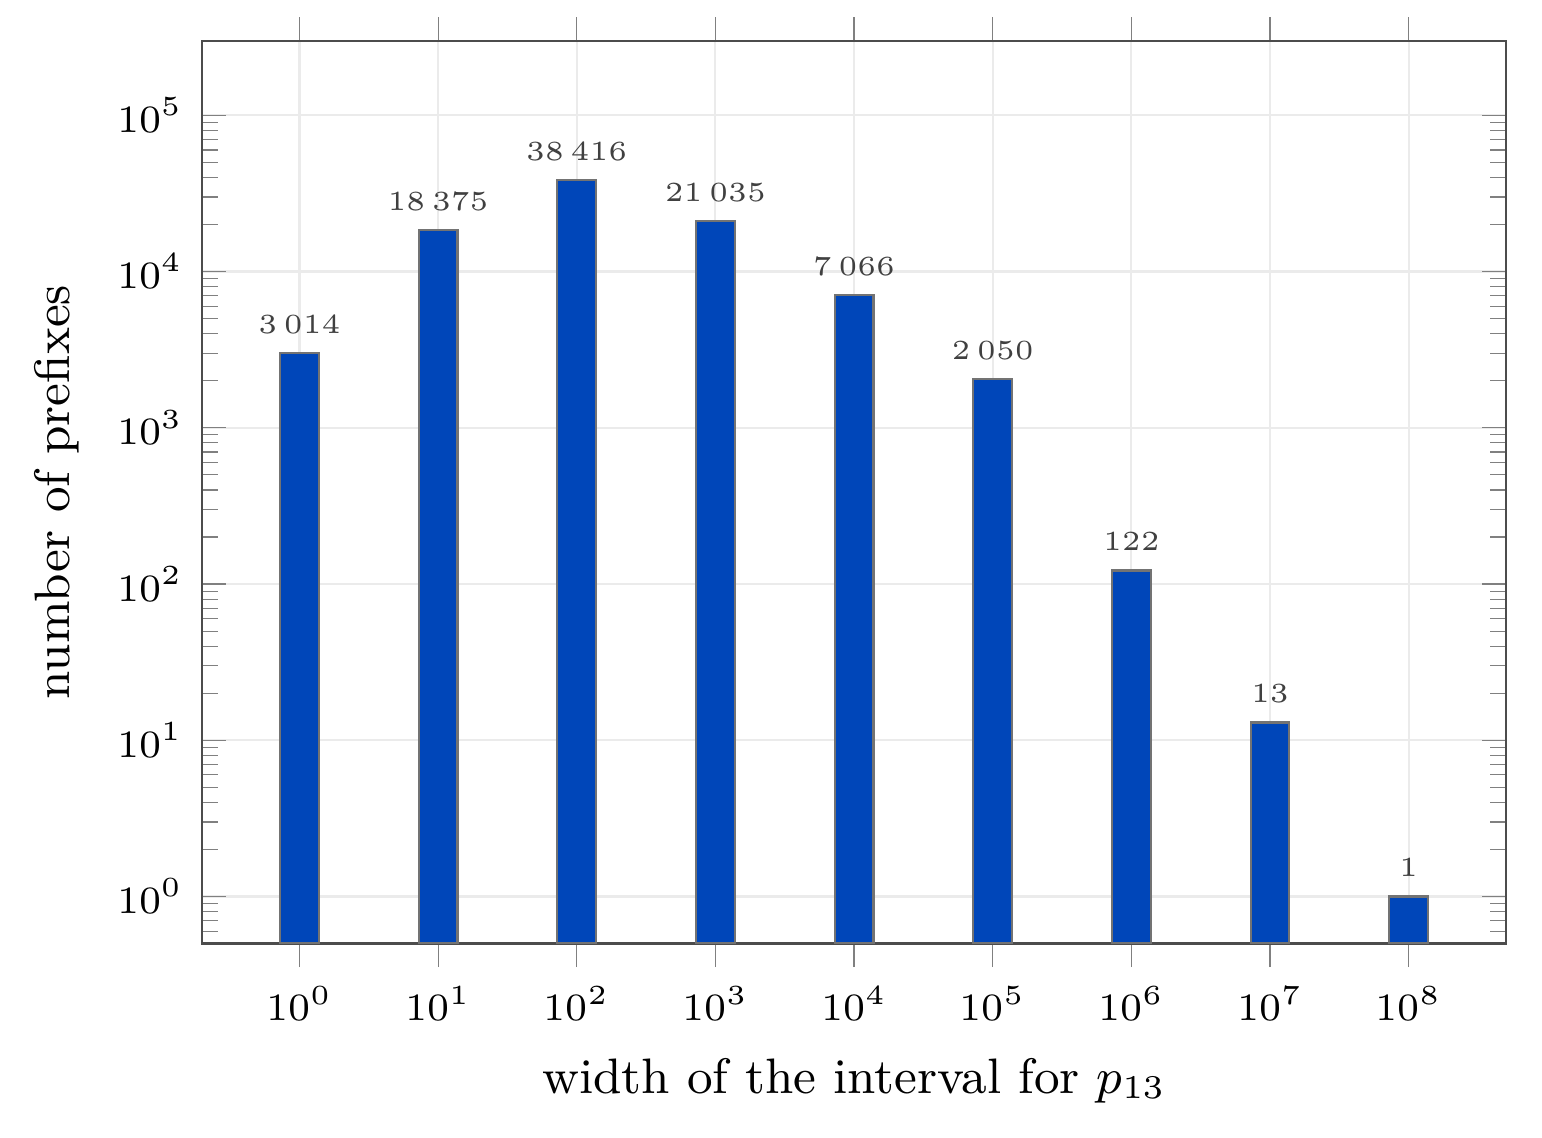
\includegraphics[width=0.62\textwidth]{figures/fig_walls.png}
\caption{The $90092$ prefixes of twelve primes for $n-1=2\varphi(n)$
with $k=16$, by the width of the interval for $p_{13}$, on logarithmic
axes. The single prefix in the last bar ends in $25867$.}
\label{fig:walls}
\end{figure}

\subsection{The companion equation with nine primes}
For \eqref{eq:second}, Theorems~\ref{thm:eight} and \ref{thm:coprime}
leave open the solutions with $3\mid n$ and $\omega(n)\ge9$, and those
with $3\nmid n$ and $\omega(n)\ge16$. In the first family the Fermat
primes make the next case far harder than the last. Under the prefix
$3,5,17,257,65537$ every admissible $p_6=s$ now leaves three primes to
choose, and the shortfall after six primes is $c/A'$ with $c=s-2^{32}$
and $A'=(2^{32}-1)s$, so that the interval for $p_7$ runs from about
$A'/c$ to $3A'/c$. Near the lower end of the interval for $p_6$ this
is an interval of length about $10^{18}$. Counting the admissible
primes $s$ exactly up to $s=2^{32}+10^7$ and estimating the rest, and
counting the primes $p_7$ with density $1/\log x$ and the share of
them that passes the prune, gives some $1.6\cdot10^{17}$ two-prime
problems from this one prefix, each with an integer $N$ of between
$60$ and $75$ digits. At a microsecond per problem this would take five
thousand years of processor time, so the case $k=9$ with $3\mid n$ is
out of reach of these methods.

\subsection{Pseudo-solutions}
Apart from the primality tests, the traversal of Section~\ref{sec:search}
uses only the following properties of the tuple $(p_1,\dots,p_k)$:
its entries are odd and increasing, they satisfy
\begin{equation}\label{eq:product}
  x_1x_2\cdots x_k+\varepsilon=2(x_1-1)(x_2-1)\cdots(x_k-1),
\end{equation}
and $\gcd(x_i,x_j-1)=1$ for all $i$ and $j$. Indeed the proofs of
Propositions~\ref{prop:below2}, \ref{prop:bounds} and~\ref{prop:last}
use nothing else once $\varphi(n)$ is replaced by
$\prod_i(x_i-1)$. We call a tuple with these properties a
\emph{pseudo-solution} if not all its entries are prime.

\begin{proposition}\label{prop:pseudo}
Let $n_0=p_1\cdots p_m$ be a Fermat-type solution with $m\ge2$ prime
factors $p_1<\dots<p_m$. Then $(p_1,\dots,p_m,n_0)$ is a
pseudo-solution of \eqref{eq:product} with $\varepsilon=-1$.
\end{proposition}

\begin{proof}
The entries are odd and increasing, and $n_0$ is composite. Since $n_0$
is squarefree, $\prod_i(p_i-1)=\varphi(n_0)=(n_0+1)/2$, and so
\[
  p_1\cdots p_m\,n_0-1=n_0^2-1=2\cdot\frac{n_0+1}{2}\cdot(n_0-1)
  =2\prod_{i\le m}(p_i-1)\cdot(n_0-1).
\]
Lemma~\ref{lem:basic}(ii), applied to $n_0$ with $\varepsilon=+1$,
gives $p_i\nmid p_j-1$ for all $i,j\le m$; hence $\gcd(p_i,p_j-1)=1$
and, as $n_0$ is the product of the $p_i$, $\gcd(n_0,p_j-1)=1$.
Finally $\gcd(n_0,n_0-1)=1$, and so $\gcd(p_i,n_0-1)=1$ because
$p_i\mid n_0$.
\end{proof}

The six Fermat-type solutions in \eqref{eq:known} with at least two
prime factors give pseudo-solutions with $k=3,4,5,6,6,7$ entries, the
smallest being $(3,5,15)$, for which $3\cdot5\cdot15-1=224=2\cdot2\cdot4\cdot14$.
Run with $\varepsilon=-1$ and $p_{\min}=3$, the search of
Section~\ref{sec:search} reaches each of them as a lattice point on
the hyperbola \eqref{eq:hyperbola} and rejects it only because its last
entry is composite. In the proof of Theorem~\ref{thm:first} they never
arise, because Lemma~\ref{lem:three} excludes $3\mid n$, and that lemma uses primality once more: its proof uses that a prime
other than $3$ is prime to $3$, and the entry $15$ is not.
Consequently no argument that uses only \eqref{eq:product}, the order
of the entries and the conditions $\gcd(x_i,x_j-1)=1$ can exclude
solutions of $n-1=2\varphi(n)$ with $k$ prime factors for any $k$ with
$3\le k\le7$; the primality of the entries has to enter the argument.

\subsection{Pseudo-solutions prime to \texorpdfstring{$3$}{3}}
The conditions $\gcd(x_i,x_j-1)=1$ are consequences of
\eqref{eq:product}, since a common divisor of $x_1\cdots x_k$ and
$\prod_j(x_j-1)$ divides $\varepsilon$. What separates the
pseudo-solutions of Proposition~\ref{prop:pseudo} from solutions of
Lehmer's equation is the prime $3$.

\begin{lemma}\label{lem:parity}
Let $x_1,\dots,x_k$ be integers with
$x_1\cdots x_k+\varepsilon=M\prod_i(x_i-1)$, where
$\varepsilon=\pm1$, and suppose that exactly $s\ge1$ of them are
divisible by $3$. Then $\varepsilon\equiv(-1)^sM\pmod3$. In particular
a solution of \eqref{eq:product} has $s$ even if $\varepsilon=-1$, and
$s=0$ or $s$ odd if $\varepsilon=+1$.
\end{lemma}

\begin{proof}
A common divisor of $x_i$ and $x_j-1$ divides both $x_1\cdots x_k$ and
$M\prod_i(x_i-1)$, hence $\varepsilon$, so $\gcd(x_i,x_j-1)=1$ for all
$i$ and $j$. Let $3\mid x_i$. Then no $x_j$ is congruent to $1$ modulo
$3$. Hence $x_j-1\equiv-1\pmod3$ if $3\mid x_j$
and $x_j-1\equiv1\pmod3$ otherwise, and the equation modulo $3$ reads
$\varepsilon\equiv(-1)^sM$. For $M=2$ this is
$\varepsilon\equiv(-1)^{s+1}$.
\end{proof}

For $s=1$ this is the congruence of Lemma~\ref{lem:three}. Each
pseudo-solution of Proposition~\ref{prop:pseudo} has $s=2$, since $3$
divides both $p_1$ and $n_0$, whereas the prime factors of $n$ give
$s\le1$. The fact that $3$ divides at most one prime factor therefore
removes all of them, and by Lemma~\ref{lem:parity} a pseudo-solution
of Lehmer's equation with pairwise coprime entries has $s=0$. We call
a pseudo-solution with $s=0$ \emph{prime to $3$}.

\begin{theorem}\label{thm:pseudo3}
Let $\varepsilon=\pm1$.
\begin{enumerate}
\item[(i)] No pseudo-solution of \eqref{eq:product} with $k\le13$ is
prime to $3$.
\item[(ii)] For $k\le15$ no pseudo-solution of \eqref{eq:product} prime
to $3$ has $x_1,\dots,x_{k-3}$ prime.
\end{enumerate}
\end{theorem}

\begin{proof}
The proofs of Propositions~\ref{prop:below2}, \ref{prop:bounds}
and~\ref{prop:last} use only \eqref{eq:product} and the order of the
entries, so the traversal of Section~\ref{sec:search} applies to odd
integers prime to $3$, with the congruence prune replaced by
$x\not\equiv0$ modulo the odd primes of $B_j$ and $x\not\equiv1$ modulo
the primes of $A_j$. For (i) the tree is traversed with integer entries
down to depth $k-3$; for $k=12$ it has $489$ nodes at that depth, below
which lie $55423$ admissible values of $x_{k-2}$. For (ii) the
traversal with prime entries is run to depth $k-3$. For $k\le12$ in
(i), and for every $k$ in (ii), every admissible odd $x_{k-2}$ prime to
$3$ in the interval is followed by the sum route of
Section~\ref{sec:sum}, which does not use primality. For $k=15$ in
(ii) these are $1.43\cdot10^8$ values of $x_{k-2}$ for each sign,
treated in about four minutes per sign; for eight of them per sign the
route would be long, and there $2AB+\varepsilon C$ is factored
completely, with every prime factor proved prime. No completion occurs.

For $k=13$ in (i) the tree has $86459$ nodes at depth $10$, the same
for both signs. Their intervals for $x_{11}$ have total length
$1.07\cdot10^{11}$ and contain $1.64\cdot10^{10}$ admissible values;
the longest, of length $1.9\cdot10^{10}$, belongs to the prefix
$5,7,13,17,19,23,25,37,119,147089$. These values are treated by the
program of Section~\ref{sec:eight}, with the conditions on primes
replaced by those of the integer prune: modulo $2$, modulo $3$ and
modulo the odd primes of $B_{10}$ the residue $0$ is excluded, and
modulo the primes of $A_{10}$ the residue $1$. Every completion in odd
integers prime to $3$ avoids these residues, because
$\gcd(x_i,x_j-1)=1$, so the sieve loses none of them. For $73106$
values, near the lower ends of the longest intervals, the integer
$2AB+\varepsilon C$, of up to $54$ digits, is factored completely
instead, with every prime factor proved prime. The program chooses
these values from its estimate of the running time, which depends on
$\varepsilon$ only through the term $\varepsilon C$, negligible beside
$2AB$; it chooses the same $73106$ values for both signs. The run took
about $15$ hours of processor time per sign, $2.5$ of them in PARI/GP,
and found no completion in odd integers prime to $3$ for either sign.
A second program factors each integer $2AB+\varepsilon C$ completely
with PARI/GP \cite{PARI}, proves every prime factor prime, and runs through all its
divisors in the class of Proposition~\ref{prop:class}. It traverses
the integer tree independently, with its own bounds, and repeats (i)
for $k\le12$; it repeats (ii) for $k\le14$, including all $67626$ values of $x_{11}$
at $k=14$, with the same result. The case $k=13$ of (i) rests on the
program of Section~\ref{sec:eight} and its checks in
Section~\ref{sec:checks8}. Allowed to use the entry $3$, the
second program finds $1$, $1$, $2$, $8$ and $47$ solutions of
\eqref{eq:product} in odd integers with $\varepsilon=-1$ for
$k=3,\dots,7$, all with $s\in\{2,4\}$, and $1$, $1$, $2$, $4$ and $18$
with $\varepsilon=+1$, all with $s$ odd; the first program, run on
prime prefixes, finds exactly those whose first $k-3$ entries are
prime.
\end{proof}

Theorem~\ref{thm:pseudo3} says that for $k\le13$ the search behind
Theorem~\ref{thm:first}, which solves \eqref{eq:product} with
$\varepsilon=-1$ and $x_1\ge5$, needs no primality beyond the fact
that $3$ divides at most one prime factor, and that for $k\le15$ it
needs the primality of the first $k-3$ factors only.

Tuples of this kind have also been studied by Molnar and Singh
\cite{MS25}, who call integers $x_1,\dots,x_r\ge2$, not necessarily
distinct, with $\prod_i(x_i-1)$ dividing $\prod_ix_i-1$ a spoof Lehmer
factorisation. They give an algorithm that finds all of them with a
given number of entries, and report ten with odd entries and at most
six of them \cite[Theorem~1.2]{MS25}. The computation in the proof of
Theorem~\ref{thm:pseudo3} gives twelve with distinct odd entries, at
most six of them and quotient $2$ alone, namely the solutions of
\eqref{eq:product} with $\varepsilon=-1$ and $3\le k\le6$. Among them
are the six-entry tuples
\begin{gather*}
  (3,5,17,257,65717,23794275),\quad (3,5,17,257,68975,1314417),\\
  (3,5,17,353,929,83623935),\quad (3,5,17,377,1217,2295),\\
  (3,5,17,395,1059,2303),\quad (3,5,33,53,69,8343),
\end{gather*}
each of which satisfies $x_1\cdots x_6-1=2(x_1-1)\cdots(x_6-1)$, as
direct multiplication shows. Together with $(3,3)$, $(3,3,3,3)$ and
$(5,5,9,9,89)$, which have repeated entries, there are at least fifteen
odd spoof Lehmer factorisations with at most six entries.

\subsection{Congruences}
The next proposition shows that Lemma~\ref{lem:three} is the only
obstruction to completing a prefix that a fixed modulus can detect.

\begin{proposition}\label{prop:local}
Let $x_1<\dots<x_j$ be odd integers such that $A=\prod x_i$ and
$B=\prod(x_i-1)$ are coprime, let $m\ge2$, and let $l^e$ be a power of
a prime $l$. Unless $l=3$, $3\mid A$ and $2B\not\equiv\varepsilon\pmod3$,
there are integers $y_1,\dots,y_m$, none divisible by $l$ and, if
$l\mid A$, none congruent to $1$ modulo $l$, such that
\[
  A\,y_1\cdots y_m+\varepsilon\equiv2B\prod_{i\le m}(y_i-1)\pmod{l^e}.
\]
In the excluded case no such integers exist.
\end{proposition}

\begin{proof}
If $l\nmid A$, take $y_1=\dots=y_{m-1}=1$ and $y_m$ with
$Ay_m\equiv-\varepsilon\pmod{l^e}$. If $l\mid A$, then $l\nmid2B$. Take
$y_3=\dots=y_m=2$ and $y_2=1+u$, where $u\in\{1,2\}$ and
$l\nmid2Bu+\varepsilon$. Such a $u$ exists, since $l$ cannot divide
both $2B+\varepsilon$ and $4B+\varepsilon$; for $l=3$ we take $u=1$,
which is allowed because $2B+\varepsilon\equiv2\varepsilon\pmod3$ by
hypothesis. Then $y_2,\dots,y_m$ are prime to $l$ and not congruent to
$1$ modulo $l$. The congruence is then linear in
$y_1$ with coefficient $K=2^{m-2}A(1+u)-2Bu\equiv-2Bu\not\equiv0\pmod
l$, so it has a solution $y_1$. Reducing modulo $l$ gives
$Ky_1\equiv-(2Bu+\varepsilon)$, so $l\nmid y_1$, and
$K(y_1-1)\equiv-\varepsilon$, so $y_1\not\equiv1$. In the excluded
case every $y_i$ is congruent to $2$ modulo $3$, so $y_i-1\equiv1$,
and the congruence modulo $3$ reads $\varepsilon\equiv2B$.
\end{proof}

By the Chinese remainder theorem the same holds for every modulus. The
integers $y_i$ satisfy every condition modulo $l$ that the prune
imposes on the remaining primes, namely $y\not\equiv0$ modulo the primes
of $B$ and $y\not\equiv1$ modulo the primes of $A$. So no congruence
condition removes a node with at least two primes left, except that of
Lemma~\ref{lem:three}; with one prime left, Proposition~\ref{prop:last}
imposes the condition $C\mid A+\varepsilon$, whose modulus is the
prefix-dependent integer $C$.

\subsection{What a proof for all \texorpdfstring{$k$}{k} has to use}
The obstruction in both cases is arithmetic. A prefix whose product
$\prod p/(p-1)$ comes very close to $2$ forces the remaining primes to
be very large and leaves them very free. For \eqref{eq:second} the
Fermat primes give the extreme example, with a shortfall of $2^{-31}$
after five primes, and every prefix near them inherits a shortfall of
the same order. By Proposition~\ref{prop:local} no congruence condition
removes such a prefix.

For the companion equation with $3\mid n$ the tuple
$(3,5,17,257,65537,2^{32}+1)$ is a pseudo-solution with pairwise
coprime entries and $s=1$. It is excluded only by the factorisation
$2^{32}+1=641\cdot6700417$, since $641-1$ does not divide
$n+1=2^{64}$, so a proof for all $k$ has to use the primality of the
large entries.

For Lehmer's equation, and for the companion equation with $3\nmid n$,
the situation is different. A solution of Lehmer's equation with
$M=2$ has $3\nmid n$ by Lemma~\ref{lem:three}, so its prime factors
form a solution of \eqref{eq:product} prime to $3$, and the same holds
for a solution of the companion equation with $M=2$ and $3\nmid n$. So
if
\eqref{eq:product} has no solution in odd integers prime to $3$, prime
or not, then neither equation has a solution with $M=2$ and
$3\nmid n$. This hypothesis involves no primes at all.
Theorem~\ref{thm:pseudo3} verifies it for $k\le13$. A first-moment count
along the tree, weighting each two-entry problem by the expected number
of divisors of $2AB+\varepsilon C$ in its class, predicts $0.8$, $1.7$,
$5.2$ and about $25$ pseudo-solutions of Lehmer's equation with the
entry $3$ allowed for $k=4,\dots,7$, against the true $1$, $2$, $8$
and $47$. For pseudo-solutions prime to $3$ it gives $4.3\cdot10^{-6}$
for $k=12$, almost all of it below the prefix
$5,7,13,17,19,23,25,37,119$, which has the smallest value
$C_9=2529647$ among the $910$ prefixes of length nine in the tree for
$k=13$. Below that prefix it gives $4\cdot10^{-6}$, $5\cdot10^{-5}$
and $2\cdot10^{-4}$ for $k=12$, $13$ and $14$.
Theorem~\ref{thm:pseudo3} is therefore what the count predicts. For larger $k$ the hypothesis fails.

\begin{theorem}\label{thm:pseudo25}
There are pseudo-solutions of \eqref{eq:product} prime to $3$ with
$\varepsilon=+1$ for every $k\ge25$, and with $\varepsilon=-1$ for
every $k\ge26$.
\end{theorem}

\begin{proof}
Let $(x_1,\dots,x_k)$ be a pseudo-solution prime to $3$ with
$\varepsilon=+1$, and write $A=x_1\cdots x_k$ and
$B=\prod_i(x_i-1)$, so that $A+1=2B$. Suppose that $3\mid B$. Every
$x_i-1$ divides $B$, so $x_k\le B+1<A<2B+1$, and
$\gcd(A,2B)=\gcd(A,A+1)=1$.

Append $x=2B+1$. Then $x$ is odd and $x\equiv1\pmod3$; it is prime to
every $x_j-1$, since $\gcd(x,B)=1$; and $x-1=2B$ is prime to every
$x_i$ and to $x$. Moreover
\[
  Ax+1=2AB+A+1=2B(A+1)=2\prod_i(x_i-1)\cdot(x-1),
\]
so the new tuple is a pseudo-solution prime to $3$ with
$\varepsilon=+1$, and $3$ divides $B(x-1)$.

Append $x=A$ instead. Then $x$ is odd and prime to $3$, it is prime
to every $x_j-1$ because $\gcd(A,B)=1$, and $x-1=A-1$ is prime to every
$x_i$ and to $x$. Moreover $A\cdot A-1=(A+1)(A-1)=2B(A-1)$, so the
new tuple is a pseudo-solution prime to $3$ with $\varepsilon=-1$.

By induction it suffices to give one pseudo-solution prime to $3$
with $\varepsilon=+1$, $k=25$ and $3\mid B$. Its first nine entries
are the prefix $5,7,13,17,19,23,25,37,119$ named above, so $3\mid B$
and the entry $25$ is composite. The remaining sixteen entries have
between $6$ and $131176$ digits, and the product has $262353$ digits.
After $24$ entries the defect $2B-A$ equals $29$, and $29$ divides
$2B+1$; the last entry is $(2B+1)/29$. The entries are deposited with
the data. The equation, the order of the entries, their residues
modulo $2$ and $3$, and all $625$ conditions $\gcd(x_i,x_j-1)=1$ are
checked by two independent programs, one in Python and one in
PARI/GP \cite{PARI}, and by the Lean kernel.
\end{proof}

The tuple was found by a search along the tree of
Theorem~\ref{thm:pseudo3}. A prefix $x_1,\dots,x_j$ with $3\mid B$
and defect $c=2B-A>0$ is completed by the entry
$X=(2B+\varepsilon)/c$ whenever $c$ divides $2B+\varepsilon$ and
$X>x_j$, because $X$ then satisfies every other condition: it is odd
and prime to $3$, $\gcd(X,B)$ divides $\varepsilon$, and
$X-1=(A+\varepsilon)/c$ is prime to $A$. Appending $x$ to a prefix gives the defect
$cx-2B$, so the defects of its children form an arithmetic progression
with difference $c$. Starting from the prefixes of the tree for $k=13$,
the search kept at each depth the $10^7$ admissible children with the
smallest defect and tested each of them. The sum of $1/c$ over the
prefixes kept at one step, which estimates the number of completions,
grew by a factor of about $2.4$ per step, and its total over all steps
first exceeded $1$ at the fourteenth step, where the completion above
occurred.

None of these tuples has pairwise coprime entries, and the search
does not reach such tuples. Among the $910$ prefixes of length $9$ of
the tree for $k=13$ with positive defect the smallest defect is
$2529647$, while among the $48$ of them with pairwise coprime entries
it is $8544556193$. The traversal of the tree for $k=15$ with
pairwise coprime entries visits $63663$ nodes, and the $13190$
prefixes among them with $0<cx_j<2B$, which one more entry can
complete, have a sum of $1/c$ of $7.7\cdot10^{-11}$, against $1.4\cdot10^{-6}$ for the $26821$ prefixes from which the
search above started. Moreover only about seven per cent of the
children of a prefix are admissible and prime to every earlier entry,
against fourteen per cent without the second condition. Run from these
prefixes with $10^6$ children kept at each step, the search finds the
sum of $1/c$ falling by a factor of about $0.8$ per step, and no
completion in twelve steps.

Solutions of \eqref{eq:product} with $\varepsilon=+1$ give solutions
with $\varepsilon=-1$ through the analogue of
Theorem~\ref{thm:ext}(ii).

\begin{proposition}\label{prop:lehmerext}
Let $(x_1,\dots,x_k)$ satisfy \eqref{eq:product} with
$\varepsilon=+1$, let $A=x_1\cdots x_k$, and let $A^2+A-1=de$ with
$1\le d<e$. Then $(x_1,\dots,x_k,A+1+d,A+1+e)$ satisfies
\eqref{eq:product} with $\varepsilon=-1$. If $x_1,\dots,x_k$ are
pairwise coprime, then so are all $k+2$ entries if and only if
$\gcd(d^2-1,A)=\gcd(d-1,A+2)=1$, and this fails whenever $5\mid A$.
\end{proposition}

\begin{proof}
Write $X=A+1+d$ and $Y=A+1+e$. Since $2\prod_i(x_i-1)=A+1$, the
equation for the longer tuple reads $AXY-1=(A+1)(X-1)(Y-1)$, which is
equivalent to $(X-A-1)(Y-A-1)=A^2+A-1$, as in the proof of
Theorem~\ref{thm:ext}; the entries increase because $x_k\le A<X<Y$.
Since $de\equiv-1\pmod A$, the integer $d$ is prime to $A$, so
$\gcd(X,A)=\gcd(d+1,A)$ and $\gcd(Y,A)=\gcd(d(e+1),A)=\gcd(d-1,A)$.
A prime $r$ dividing $X$ and $Y$ has $d\equiv e\equiv-(A+1)$, hence
$(A+1)^2\equiv A^2+A-1$, that is $A\equiv-2$ and $d\equiv1\pmod r$;
conversely, if $r$ divides $A+2$ and $d-1$, then
$e\equiv de=A^2+A-1\equiv1$, and $r$ divides $X$ and $Y$. Finally let
$5\mid A$. Every prime factor $r$ of $A^2+A-1$ is odd and different
from $5$, and $(2A+1)^2\equiv5\pmod r$, so $5$ is a square modulo $r$
and, by quadratic reciprocity, $r\equiv\pm1\pmod5$. Hence
$d\equiv\pm1\pmod5$, and $5$ divides $\gcd(d^2-1,A)$.
\end{proof}

For the Fermat numbers $3,5,17,257,65537,2^{32}+1$,
Proposition~\ref{prop:lehmerext} gives pseudo-solutions of Lehmer's
equation with $s=2$, and none with pairwise coprime entries, because
$3$ and $5$ divide $A$. Appending $2B+1=A+2$, as in the proof of
Theorem~\ref{thm:pseudo25}, keeps the entries pairwise coprime, so a
single pairwise coprime pseudo-solution of the companion equation
prime to $3$ with $3\mid B$ would give infinitely many, and
Proposition~\ref{prop:lehmerext} turns every divisor $d$ of $A^2+A-1$
with $\gcd(d^2-1,A)=\gcd(d-1,A+2)=1$ into a pseudo-solution of
Lehmer's equation with pairwise coprime entries. By
Lemma~\ref{lem:parity} a pseudo-solution of Lehmer's equation with
pairwise coprime entries is prime to $3$, and we do not know whether
one exists. The smallest $k$ with a pseudo-solution prime to $3$ lies
between $14$ and $25$ for $\varepsilon=+1$, and between $14$ and $26$
for $\varepsilon=-1$.



\appendix
%%==================================================================
\section{Solutions used in the checks}\label{app:known}
%%==================================================================

The following $56$ integers $n=p_1\cdots p_k$ satisfy
$2^k(n-1)=(2^k+m)\varphi(n)$ for the indicated $m$. They are the
complete output of both implementations for $k=4$, $1\le m\le40$, and
$k=5$, $1\le m\le85$, with $p_1\ge3$, listed in increasing order of
$n$ down the columns. Each was verified by direct arithmetic.

\begin{table}[ht]
\centering
\caption{Solutions with $k=4$, $1\le m\le40$.}
\label{tab:S4}
\smallskip
\footnotesize
\begin{tabular}{@{}lr@{\qquad}lr@{}}
\toprule
$p_1,\dots,p_4$ & $m$ & $p_1,\dots,p_4$ & $m$ \\
\midrule
$3,\,5,\,47,\,89$ & 15 & $13,\,29,\,433,\,2969$ & 2 \\
$5,\,19,\,29,\,163$ & 6 & $7,\,97,\,139,\,8581$ & 3 \\
$7,\,17,\,229,\,251$ & 4 & $13,\,29,\,383,\,28879$ & 2 \\
$3,\,29,\,263,\,521$ & 9 & $11,\,47,\,1109,\,15497$ & 2 \\
$13,\,37,\,151,\,271$ & 2 & $29,\,41,\,1291,\,15199$ & 1 \\
$3,\,29,\,197,\,1559$ & 9 & $11,\,47,\,1049,\,77477$ & 2 \\
$17,\,23,\,83,\,1709$ & 2 & $7,\,61,\,859,\,183397$ & 3 \\
$29,\,71,\,163,\,193$ & 1 & $31,\,37,\,2377,\,66499$ & 1 \\
$41,\,43,\,97,\,491$ & 1 & $19,\,157,\,9697,\,15511$ & 1 \\
$37,\,41,\,137,\,829$ & 1 & $19,\,157,\,8353,\,20887$ & 1 \\
\bottomrule
\end{tabular}
\end{table}

\begin{table}[ht]
\centering
\caption{Solutions with $k=5$, $1\le m\le85$.}
\label{tab:S5}
\smallskip
\footnotesize
\begin{tabular}{@{}lr@{\qquad}lr@{}}
\toprule
$p_1,\dots,p_5$ & $m$ & $p_1,\dots,p_5$ & $m$ \\
\midrule
$5,\,7,\,13,\,139,\,653$ & 19 & $5,\,47,\,317,\,40253,\,499027$ & 9 \\
$11,\,13,\,17,\,109,\,379$ & 9 & $19,\,269,\,443,\,1747,\,1852699$ & 2 \\
$3,\,17,\,29,\,317,\,4643$ & 21 & $23,\,71,\,983,\,1031,\,103437589$ & 2 \\
$11,\,17,\,107,\,173,\,1373$ & 6 & $19,\,199,\,757,\,5059,\,23698783$ & 2 \\
$5,\,19,\,37,\,73,\,19739$ & 12 & $31,\,43,\,233,\,318629,\,12310321$ & 2 \\
$19,\,73,\,97,\,103,\,613$ & 3 & $19,\,313,\,389,\,1277,\,590838019$ & 2 \\
$11,\,17,\,127,\,131,\,2879$ & 6 & $11,\,47,\,1051,\,67967,\,102302009$ & 4 \\
$5,\,7,\,269,\,317,\,4283$ & 15 & $7,\,59,\,1721,\,41813,\,958695209$ & 6 \\
$5,\,53,\,233,\,857,\,5689$ & 9 & $41,\,167,\,14411,\,322633,\,1891541$ & 1 \\
$31,\,53,\,149,\,569,\,3407$ & 2 & $31,\,37,\,2411,\,47681,\,5732949913$ & 2 \\
$13,\,17,\,271,\,1567,\,5573$ & 5 & $31,\,37,\,2297,\,2639701,\,1379629439$ & 2 \\
$7,\,13,\,17,\,1553,\,480499$ & 11 & $37,\,463,\,827,\,1667389,\,4325665973$ & 1 \\
$17,\,23,\,131,\,199,\,167099$ & 4 & $37,\,353,\,1867,\,25109743,\,844718249$ & 1 \\
$11,\,83,\,163,\,239,\,210461$ & 4 & $43,\,139,\,61729,\,212167,\,32068788511$ & 1 \\
$13,\,167,\,349,\,1747,\,8237$ & 3 & $37,\,367,\,1553,\,21098893,\,41563512479$ & 1 \\
$19,\,181,\,1439,\,3767,\,17683$ & 2 & $43,\,139,\,47857,\,57253657,\,72147837793$ & 1 \\
$3,\,11,\,269,\,17837,\,3861929$ & 21 & $37,\,353,\,1867,\,24384917,\,20504256743083$ & 1 \\
$43,\,317,\,331,\,953,\,166357$ & 1 & $43,\,139,\,47819,\,1145259251,\,653813324977$ & 1 \\
\bottomrule
\end{tabular}
\end{table}


\section*{Data availability}
The programs that carry out the searches, the threshold computations
and the checks of Section~\ref{sec:checks}, their recorded output, the
factorisations of the fifteen integers of Table~\ref{tab:hard}, the
logs of the three-prime searches of Section~\ref{sec:fifteen}, the
program and the journal of the eight-prime search of
Section~\ref{sec:eight}, the programs and logs of
Section~\ref{sec:walls}, the entries of the tuple of
Theorem~\ref{thm:pseudo25}, the Lean formalisation of
Section~\ref{sec:lean} and the sources of this paper are archived at
Zenodo, \href{https://doi.org/\zenododoi}{doi:\zenododoi}, and
maintained at \url{https://github.com/creelie/Lehmer-1-2}. The programs and the
formal proofs were written by D.~Bhattacharjee with the assistance of
Claude, an AI system developed by Anthropic, which helped with the
coding; the authors checked the programs, the proofs and their output
and take full responsibility for them.

\begin{thebibliography}{99}

\bibitem{APR83}
L.~M. Adleman, C.~Pomerance, and R.~S. Rumely,
\emph{On distinguishing prime numbers from composite numbers},
Ann. of Math. (2) \textbf{117} (1983), no.~1, 173--206.
\href{https://doi.org/10.2307/2006975}{doi:10.2307/2006975}

\bibitem{BW80}
R.~Baillie and S.~S. Wagstaff, Jr.,
\emph{Lucas pseudoprimes},
Math. Comp. \textbf{35} (1980), no.~152, 1391--1417.
\href{https://doi.org/10.1090/S0025-5718-1980-0583518-6}{doi:10.1090/S0025-5718-1980-0583518-6}

\bibitem{BNP09}
W.~D. Banks, C.~W. Nevans, and C.~Pomerance,
\emph{A remark on Giuga's conjecture and Lehmer's totient problem},
Albanian J. Math. \textbf{3} (2009), no.~2.
\href{https://doi.org/10.51286/albjm/1245207560}{doi:10.51286/albjm/1245207560}

\bibitem{BLS75}
J.~Brillhart, D.~H. Lehmer, and J.~L. Selfridge,
\emph{New primality criteria and factorizations of $2^m\pm1$},
Math. Comp. \textbf{29} (1975), no.~130, 620--647.
\href{https://doi.org/10.1090/S0025-5718-1975-0384673-1}{doi:10.1090/S0025-5718-1975-0384673-1}

\bibitem{BCF11}
P.~Burcsi, S.~Czirbusz, and G.~Farkas,
\emph{Computational investigation of Lehmer's totient problem},
Ann. Univ. Sci. Budapest. Sect. Comput. \textbf{35} (2011), 43--49.
\href{https://doi.org/10.71352/ac.35.043}{doi:10.71352/ac.35.043}

\bibitem{CH80}
G.~L. Cohen and P.~Hagis, Jr.,
\emph{On the number of prime factors of $n$ if $\varphi(n)\mid(n-1)$},
Nieuw Arch. Wisk. (3) \textbf{28} (1980), 177--185.

\bibitem{CL84}
H.~Cohen and H.~W. Lenstra, Jr.,
\emph{Primality testing and Jacobi sums},
Math. Comp. \textbf{42} (1984), no.~165, 297--330.
\href{https://doi.org/10.1090/S0025-5718-1984-0726006-X}{doi:10.1090/S0025-5718-1984-0726006-X}

\bibitem{CHN08}
D.~Coppersmith, N.~Howgrave-Graham, and S.~V. Nagaraj,
\emph{Divisors in residue classes, constructively},
Math. Comp. \textbf{77} (2008), no.~261, 531--545.
\href{https://doi.org/10.1090/S0025-5718-07-02007-8}{doi:10.1090/S0025-5718-07-02007-8}

\bibitem{FG}
J.~Feitsma and W.~Galway,
\emph{Tables of pseudoprimes and related data},
\url{https://www.cecm.sfu.ca/Pseudoprimes/index-2-to-64.html}.

\bibitem{FLINT}
The FLINT team,
\emph{FLINT: Fast Library for Number Theory}, version~3.6.0,
\url{https://flintlib.org}.

\bibitem{Guy04}
R.~K. Guy,
\emph{Unsolved Problems in Number Theory}, 3rd ed.,
Problem Books in Mathematics, Springer, New York, 2004.
\href{https://doi.org/10.1007/978-0-387-26677-0}{doi:10.1007/978-0-387-26677-0}

\bibitem{Hag88}
P.~Hagis, Jr.,
\emph{On the equation $M\cdot\varphi(n)=n-1$},
Nieuw Arch. Wisk. (4) \textbf{6} (1988), no.~3, 255--261.

\bibitem{Leh32}
D.~H. Lehmer,
\emph{On Euler's totient function},
Bull. Amer. Math. Soc. \textbf{38} (1932), no.~10, 745--751.
\href{https://doi.org/10.1090/S0002-9904-1932-05521-5}{doi:10.1090/S0002-9904-1932-05521-5}

\bibitem{Len84}
H.~W. Lenstra, Jr.,
\emph{Divisors in residue classes},
Math. Comp. \textbf{42} (1984), no.~165, 331--340.
\href{https://doi.org/10.1090/S0025-5718-1984-0726007-1}{doi:10.1090/S0025-5718-1984-0726007-1}

\bibitem{Mathlib}
The mathlib Community,
\emph{The Lean mathematical library},
in: Proceedings of the 9th ACM SIGPLAN International Conference on
Certified Programs and Proofs (CPP 2020), ACM, New York, 2020, 367--381.
\href{https://doi.org/10.1145/3372885.3373824}{doi:10.1145/3372885.3373824}

\bibitem{SymPy}
A.~Meurer, C.~P. Smith, M.~Paprocki, O.~\v{C}ert\'{\i}k, S.~Kirpichev,
et al., \emph{SymPy: symbolic computing in Python},
PeerJ Comput. Sci. \textbf{3} (2017), e103.
\href{https://doi.org/10.7717/peerj-cs.103}{doi:10.7717/peerj-cs.103}

\bibitem{MS25}
G.~Molnar and G.~Singh,
\emph{Positive spoof Lehmer factorizations},
preprint, 2025, arXiv:2409.17076v2 [math.NT].
\href{https://doi.org/10.48550/arXiv.2409.17076}{doi:10.48550/arXiv.2409.17076}

\bibitem{Lean4}
L.~de Moura and S.~Ullrich,
\emph{The Lean~4 theorem prover and programming language},
in: Automated Deduction -- CADE~28, Lecture Notes in Comput. Sci.
\textbf{12699}, Springer, Cham, 2021, 625--635.
\href{https://doi.org/10.1007/978-3-030-79876-5_37}{doi:10.1007/978-3-030-79876-5\_37}

\bibitem{OEIS}
OEIS Foundation Inc.,
\emph{The On-Line Encyclopedia of Integer Sequences},
sequences A050474 and A203966, \url{https://oeis.org}, accessed
September 2026.

\bibitem{PARI}
The PARI~Group,
\emph{PARI/GP}, version~2.15.4, Univ. Bordeaux,
\url{https://pari.math.u-bordeaux.fr}.

\bibitem{Pin06}
R.~G.~E. Pinch,
\emph{A note on Lehmer's totient problem},
poster, Seventh Algorithmic Number Theory Symposium (ANTS~VII), Berlin, 2006.
\url{https://antsmath.org/ANTSVII/Poster/Pinch_Poster3.pdf}

\bibitem{Pom77}
C.~Pomerance,
\emph{On composite $n$ for which $\varphi(n)\mid n-1$, II},
Pacific J. Math. \textbf{69} (1977), no.~1, 177--186.
\href{https://doi.org/10.2140/pjm.1977.69.177}{doi:10.2140/pjm.1977.69.177}

\bibitem{PSW80}
C.~Pomerance, J.~L. Selfridge, and S.~S. Wagstaff, Jr.,
\emph{The pseudoprimes to $25\cdot10^9$},
Math. Comp. \textbf{35} (1980), no.~151, 1003--1026.
\href{https://doi.org/10.1090/S0025-5718-1980-0572872-7}{doi:10.1090/S0025-5718-1980-0572872-7}

\bibitem{Ren04}
J.~Renze,
\emph{Computational evidence for Lehmer's totient conjecture},
Mathematica notebook, Wolfram Library Archive, MathSource item 5483, 2004.
\url{https://library.wolfram.com/infocenter/MathSource/5483/}

\bibitem{SW17}
J.~Sorenson and J.~Webster,
\emph{Strong pseudoprimes to twelve prime bases},
Math. Comp. \textbf{86} (2017), no.~304, 985--1003.
\href{https://doi.org/10.1090/mcom/3134}{doi:10.1090/mcom/3134}

\bibitem{Won97}
E.~Wong,
\emph{Computations on normal families of primes},
M.Sc. thesis, Simon Fraser University, 1997.

\end{thebibliography}


\end{document}
